\documentclass[12pt]{book}
\usepackage[paperwidth=17cm, paperheight=22.5cm, bottom=2.5cm, right=2.5cm]{geometry}
\usepackage{amssymb,amsmath,amsthm} %paquete para símbolo matemáticos
%\usepackage[spanish,english]{babel}
\usepackage[spanish]{babel}
\usepackage[utf8]{inputenc} %Paquete para escribir acentos y otros símbolos directamente
\usepackage{enumerate}
\usepackage{graphicx}
\usepackage[table]{xcolor}
%\usepackage{subfig} %para poner subfiguras
\graphicspath{{Img/}} %En qué carpeta están las imágenes
\usepackage[nottoc]{tocbibind}
\usepackage[pdftex,
            pdfauthor={NOMBRE DEL AUTOR},
            pdftitle={TÍTULO DE LA TESIS},
            pdfsubject={ÁREA DE LA TESIS},
            pdfkeywords={PALABRAS CLAVE},
            pdfproducer={Latex con hyperref},
            pdfcreator={pdflatex}]{hyperref}

\usepackage{blindtext}
\usepackage{hyperref}

\usepackage{svg}
\usepackage{listings}

\begin{document}

%----------------------------------------------------------------------------------------
%	COMANDOS PERSONALIZADOS
%----------------------------------------------------------------------------------------

%Para teoremas y demostraciones 

\renewcommand{\proofname}{Demostración}
\providecommand{\norm}[1]{\lVert#1\rVert} %Provee el comando para producir una norma.
\providecommand{\innp}[1]{\langle#1\rangle} 
\newcommand{\seno}{\mathrm{sen}}
\newcommand{\diff}{\mathrm{d}}

\newtheorem{teo}{Teorema}[section] 
\newtheorem{cor}[teo]{Corolario}
\newtheorem{lem}[teo]{Lema}

\theoremstyle{definition}
\newtheorem{dfn}[teo]{Definición}

\theoremstyle{remark}
\newtheorem{obs}[teo]{Observación}

\allowdisplaybreaks




%----------------------------------------------------------------------------------------
%	PORTADA
%----------------------------------------------------------------------------------------

\title{TÍTULO DE LA TESIS} %Con este nombre se guardará el proyecto en writeLaTex

\begin{titlepage}
\begin{center}

%% Portada bonita
\begin{minipage}{\textwidth} 
  \newcolumntype{V}{>{\centering\arraybackslash} m{.17\textwidth} }
  \newcolumntype{C}{>{\centering\arraybackslash} m{.56\textwidth} }
  \begin{tabular}{ V C V }
  
\includegraphics[width=.15\textwidth]{UNAMlogo.png}  %
  &\Large Universidad Nacional Autónoma de México y Universidad Michoacana de San Nicolás de Hidalgo &%
  
\includegraphics[width=.15\textwidth]{UMSNHlogo.png}
 \end{tabular}
\end{minipage} 


 \vfill


\begin{minipage}{0.7\textwidth}
\begin{center}
\vspace*{0.7cm}
\large Posgrado Conjunto en Ciencias Matemáticas UMSNH-UNAM
\end{center}
\end{minipage} \\

\begin{center}
\vspace*{0.7cm}
\medskip \rule{.9\textwidth}{2pt}
\bigskip \\
AQUI VA EL TITULO DE LA TESIS \\
%{\Large \bfseries  \thetitle   }
\medskip \rule{.9\textwidth}{2pt}
\end{center}

\begin{center}
\vspace*{0.7cm}
{\huge TESIS}\\
\vspace*{0.7cm}
para obtener el grado de \\ \bigskip
{\large \emph{Maestra en Ciencias Matemáticas}} \\ \bigskip
presenta\\ \medskip
%\theauthor \\
Paula Camila Silva Gomez \\
\texttt{csilva@matmor.unam.mx}
\bigskip \\
Asesor: \\
Doctora\\
Nelly Sélem Mojica\\
\texttt{nselem@matmor.unam.mx}
\end{center}

\vfill

\begin{center}
{Morelia, Michoacán, México}\\
% {\thedate}% to use the date of compilation
{Octubre, 2023}
\end{center}

\end{center}
\end{titlepage}

%----------------------------------------------------------------------------------------
%	DECLARACIÓN
%----------------------------------------------------------------------------------------

\thispagestyle{empty}
\vspace*{\fill}
\begingroup
%``Con fundamento en los artículos 21 y 27 de la Ley Federal del Derecho de Autor y como titular de los derechos moral y patrimonial de la obra titulada ``\textbf{TÍTULO DE LA TESIS}'', otorgo de manera gratuita y permanente al Instituto Tecnológico Autónomo de México y a la Biblioteca Raúl Bailléres Jr., la autorización para que fijen la obra en cualquier medio, incluido el electrónico, y la divulguen entre sus usuarios, profesores, estudiantes o terceras personas, sin que pueda percibir por tal divulgación una contraprestación''.

\centering

\hspace{5em}

\textsc{Paula Camila Silva Gomez}

\vspace{5em}

\rule[1em]{20em}{0.5pt} % Línea para la firma

\textsc{Firma}
 
\vspace{5em}

\rule[1em]{20em}{0.5pt} % Línea para la fecha

\textsc{Fecha}

\endgroup
\vspace*{\fill}


%----------------------------------------------------------------------------------------
%	DEDICATORIA
%----------------------------------------------------------------------------------------

%\pagestyle{empty}
%\frontmatter

%\chapter*{}
%\begin{flushright}
%\textit{DEDICATORIA}
%\end{flushright}


%----------------------------------------------------------------------------------------
%	AGRADECIMIENTOS
%----------------------------------------------------------------------------------------

\chapter*{Agradecimientos}
%\markboth{AGRADECIMIENTOS23}{AGRADECIMIENTOS} % encabezado 

Gracias totales.


%----------------------------------------------------------------------------------------
%	TABLA DE CONTENIDOS
%---------------------------------------------------------------------------------------

\tableofcontents


%----------------------------------------------------------------------------------------
%	TESIS
%----------------------------------------------------------------------------------------
\chapter*{Abstract}
\thispagestyle{empty}

\chapter*{Introducción}
\thispagestyle{empty}

\mainmatter %empieza la numeración de las páginas
\pagestyle{headings}

%  Incluye los capítulos en el folder de capítulos

\chapter{Preliminares}
La ciencia de datos es el campo que aplica técnicas analíticas avanzadas y principios científicos para extraer información valiosa de los datos. Su objetivo principal es la extracción, el análisis y la comunicación de información útil a partir de los datos. Combina la estadística, la informática y el pensamiento crítico para obtener conocimiento significativo y relevante. Para realizar un análisis de datos, es necesario tener conocimientos en matemáticas, estadística, programación, inteligencia artificial, aprendizaje automático y experiencia en diversas áreas de aplicación. En este caso, es indispensable incursionar en conocimientos de genómica y metagenómica.\\

En microbiología, un factor importante de estudio son las interacciones entre microorganismos en un ambiente natural, ya que la mayoría de estos estudios se realizan en laboratorios. Los avances tecnológicos han llevado al desarrollo de métodos de secuenciación de ADN. Una de las plataformas más utilizadas y conocidas en el campo de la metagenómica es Illumina. Con este tipo de herramientas, es posible analizar el ADN extraído directamente de una muestra, en lugar de trabajar únicamente con microorganismos cultivados individualmente.\\

La filogenética es el estudio de la evolución de la vida y las relaciones entre organismos y grupos de organismos. Este análisis se centra en temas como la diversidad, la evolución, la ecología y los genomas, ayudándonos a comprender cómo evolucionan los genes, los genomas y las especies. Una parte importante de este estudio es la identificación, clasificación y denominación de organismos biológicos, campo conocido como taxonomía. Carl Linnaeus, considerado el padre de la taxonomía, propuso siete niveles taxonómicos: Reino, Phylum, Clase, Orden, Familia, Género y Especie. Posteriormente, se añadió el Dominio como el octavo grupo taxonómico más amplio, dividido en Arqueas, Bacterias y Eukarya.\\

\begin{figure}[h]
\centering
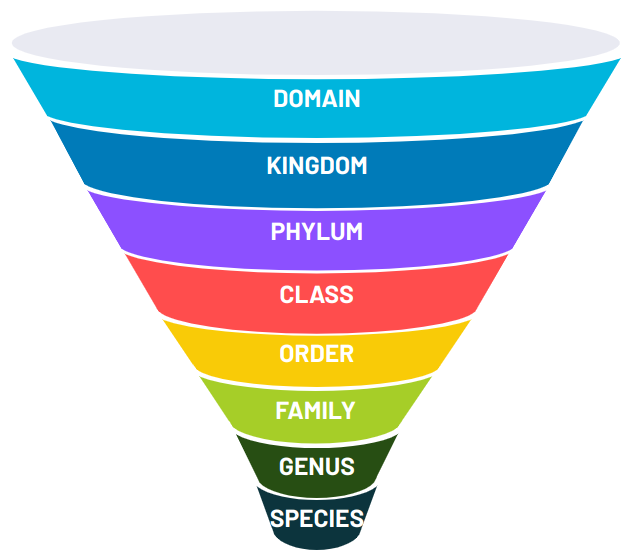
\includegraphics[scale=0.3]{Img/cap1/taxonomic.png}
\label{Fig 1.1}
\caption{Representación Jerárquica de los Niveles Taxonómicos para la Clasificación y Análisis de Datos Metagenómicos}
\end{figure}


Los niveles taxonómicos \ref{Fig 1.1} son categorías jerárquicas utilizadas para clasificar organismos, desde los grupos más generales hasta los más específicos. El Reino es el nivel más amplio y agrupa organismos según características fundamentales, como ser procariotas o eucariotas. Dentro de cada reino, los organismos se subdividen en Filos, que los organizan según estructuras o procesos biológicos compartidos. Estos se clasifican en Clases, que reúnen grupos más específicos de organismos. A su vez, las clases se dividen en Órdenes, que contienen familias relacionadas. Las Familias agrupan Géneros, que son conjuntos de especies estrechamente relacionadas. Finalmente, la Especie es el nivel más específico, que incluye organismos capaces de reproducirse entre sí y producir descendencia viable. Esta jerarquía es esencial para organizar la biodiversidad y estudiar las relaciones evolutivas entre los organismos.\\

\section{Metagenómica}
La metagenómica es el estudio integral del material genético recuperado directamente de muestras ambientales. Permite analizar el genoma colectivo (metagenoma) de todos los microorganismos presentes en un ambiente determinado, sin necesidad de cultivarlos individualmente. Este campo se centra en comprender la diversidad microbiana, las estructuras poblacionales, las capacidades funcionales y las interacciones de las comunidades microbianas con su entorno. Se aplica comúnmente en el estudio de ecosistemas como el suelo, el agua, la microbiota humana y otros hábitats microbianos complejos. La metagenómica utiliza tecnologías avanzadas de secuenciación, como la secuenciación de nueva generación, para desentrañar la diversidad genética y funcional de estas comunidades (Zhang, 2021).\\

Existen dos enfoques para la secuenciación de microorganismos: “Amplicón 16S rRNA” y “Shotgun”. La secuenciación por amplicón 16S fue el primer método de secuenciación metagenómica altamente aceptado. Tiene muchas ventajas: el gen 16S está presente en todas las bacterias y arqueas, contiene las regiones necesarias para un buen análisis de PCR (Polymerase Chain Reaction - Reacción en Cadena de la Polimerasa) altamente conservadas, existen conjuntos de primers altamente estudiados para amplificar la mayoría de los organismos, ya se encuentran disponibles bases de datos públicas y bien seleccionadas que permiten una buena comparación, y la secuenciación por 16S es relativamente barata y simple. Sin embargo, posee algunas desventajas: el gen 16S no está presente en los hongos, por lo que este método no es adecuado cuando se desea trabajar con hongos. Además, existe la posibilidad de que se incremente el error de sesgo si no se elige el conjunto de primers adecuado para el organismo a analizar.\\

Para realizar una secuenciación por 16S, es necesario seguir una serie de pasos para la preparación de la muestra biológica y la extracción del ADN: colecta de la muestra, extracción del ADN y preparación de la librería. Para la colecta de las muestras, se deben tener en cuenta las necesidades del experimento y los resultados esperados, estimar el número de muestras necesarias y considerar el método de almacenamiento; todo esto para garantizar la calidad de los datos. Existen varios métodos y herramientas para realizar la extracción del ADN. Es necesario preparar bibliotecas de datos genómicos para la comparación de las secuencias. Posteriormente, se continúa con la secuenciación de las muestras, para lo cual existen varias herramientas, siendo una de las más usadas Ilumina, que ofrece una mayor cobertura a menor costo. Finalmente, se realiza un control de calidad, cuyo principal objetivo es mejorar la precisión del análisis y prevenir la sobreestimación de los datos. El control de calidad puede incluir: la detección y eliminación de quimeras artificiales, el filtrado de secuencias de baja calidad y de reads muy cortos, así como la eliminación de ruido.\\

Una vez obtenidas las secuencias, es necesario identificar el grupo taxonómico correspondiente para cada secuencia. Para esto, se conocen dos enfoques principales: uno basado en filotipos, que agrupa las secuencias directamente en función de su similitud con los filotipos, y otro basado en OTUs (Unidades Taxonómicas Operacionales), que agrupa las secuencias según la similitud entre OTUs. El método de agrupación por OTUs supera al basado en filotipos, pero también presenta ciertas limitaciones, ya que es relativamente costoso computacionalmente y requiere mucha memoria. Un OTU se define dentro del mismo clúster por un porcentaje de similitud, siendo el 97\% un porcentaje común a nivel de especie. Estos OTUs se obtienen mediante clústering, para lo cual ya existen varios métodos y algoritmos disponibles (Xia et al., 2018).\\

\section{Microbioma}
El microbioma se define como la comunidad completa de microorganismos (incluyendo bacterias, arqueas, hongos, protozoos y virus) que habitan en un entorno específico, como el cuerpo humano, animales, plantas o ambientes naturales. Este término no solo abarca a los microorganismos vivos, sino también sus genes, metabolitos y las interacciones que tienen entre ellos y con su huésped. La investigación del microbioma utiliza herramientas avanzadas, como la secuenciación de próxima generación y los análisis metagenómicos, para entender su diversidad y funciones en la salud, la enfermedad y los ecosistemas (Marchesi \& Ravel, 2015).\\
% (Marchesi, J.R., Ravel, J. The vocabulary of microbiome research: a proposal. Microbiome 3, 31 (2015). https://doi.org/10.1186/s40168-015-0094-5) 

\section{Clasificadores}

\subsection{Kaiju}
Kaiju es un programa para clasificación taxonómica de lecturas de secuenciación de alto rendimiento,  a partir de la secuenciación del genoma completo de ADN metagenómico. \\

\subsection{Kraken \& Braken}
Kraken es una herramienta de clasificación de secuencias de ADN metagenómico mediante alineación exacta de k-mers, asignándoles etiquetas taxonómicas con gran exactitud y velocidad (Wood, 2014)(\cite{wood2014kraken}). Esta herramienta crea su base de datos de consulta a partir de una biblioteca de datos metagenómicos e información taxonómica de NCBI (National Center for Biotechnology Information).\\

Kraken deja sin clasificar las secuencias que no tienen k-mers presentes en la base de datos precalculada.\\

La salida de Kraken consiste en una línea por cada read, que contiene 5 ítems separados por tabulaciones. En primer lugar, se indica si el read fue clasificado o no clasificado (C/U), seguido por el nombre del read (ID de la secuencia, el encabezado del archivo FASTA o FASTQ de entrada), la etiqueta taxonómica asignada por Kraken (0 si la secuencia no queda clasificada), la longitud de la secuencia en pares de bases (bp), y finalmente una lista delimitada por espacios que muestra el mapeo LCA (Lowest Common Ancestor) de cada k-mer de la secuencia (ID taxonómico : número de k-mers).\\

Para obtener el ID taxonómico completo, Kraken dispone de la herramienta kraken\_translate, que, después de procesar los resultados con la misma base de datos, genera una lista de los reads junto con el nombre completo del ID taxonómico. Además, tiene una herramienta complementaria (-mpa), que presenta la salida ordenada por categoría taxonómica (root\_Super Kingdom, d\_kingdom, p\_phylum, c\_class, o\_order, f\_family, g\_genus, s\_species). (Wood \& Salzberg, 2014) .\\

%\begin{figure}[h]
%\centering
%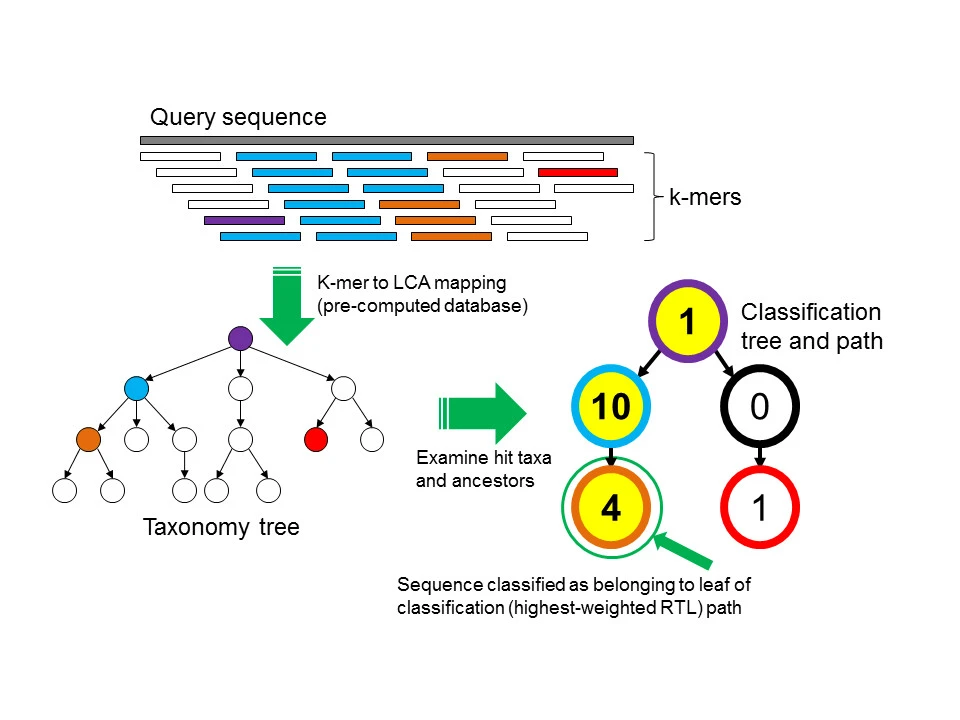
\includegraphics[scale=0.3]{Img/cap1/kraken.png}
%\caption{kraken}
%\end{figure}

BRACKEN (Bayesian Re-estimation of Abundance after Classification with KraKEN) calcula la abundancia de especies, géneros u otras categorías taxonómicas a partir de las secuencias de ADN recopiladas en un experimento de metagenómica (Lu et al., 2017)(\cite{lu2017bracken}).\\

BRACKEN realiza estimaciones probabilísticas basadas en las salidas de Kraken para completar las asignaciones al nivel taxonómico requerido, con el objetivo de obtener una estimación de abundancia más precisa. Este enfoque permite producir estimaciones fiables de abundancia a nivel de especie y género, incluso cuando una muestra contiene múltiples especies casi idénticas.\\

\section{Lenguajes}

\subsection{BASH}
Bash (Bourne Again SHell) es un intérprete de comandos y un lenguaje de scripting desarrollado para el sistema operativo Unix y sus derivados, como Linux. Creado en 1989 por Brian Fox, Bash permite automatizar tareas mediante scripts, lo que resulta particularmente útil en entornos de análisis bioinformático, donde se requiere manejar grandes volúmenes de datos. Aunque no está diseñado específicamente para análisis estadísticos o gráficos, Bash es fundamental para la gestión de flujos de trabajo y la integración de herramientas como BLAST, SAMtools y GATK. Se emplea para procesar datos en sistemas de alto rendimiento, administrar flujos de trabajo de análisis masivo y realizar manipulaciones rápidas de datos en formatos de texto o binarios. \\

\subsection{Python}
Python es un lenguaje de programación de propósito general, conocido por su sintaxis sencilla y su amplia aplicabilidad en la ciencia de datos, bioinformática y aprendizaje automático. Fue creado por Guido van Rossum en 1991 y se ha consolidado como una herramienta versátil en disciplinas científicas debido a su capacidad para integrar múltiples flujos de trabajo. Python cuenta con bibliotecas científicas robustas, como NumPy para álgebra lineal, Pandas para manejo de datos estructurados y Biopython para análisis bioinformáticos. Se emplea en la automatización de procesos, el desarrollo de algoritmos personalizados, el análisis de secuencias genómicas y la inteligencia artificial aplicada a la investigación científica.\\

\subsubsection{Phyloseq}
Phyloseq es un software de código abierto diseñado para la manipulación y análisis integral de datos metagenómicos generados mediante tecnologías de secuenciación de alto rendimiento. Esta herramienta, desarrollada en R, ofrece capacidades para importar, almacenar, analizar y visualizar datos metagenómicos de manera eficiente. En el entorno de R, los datos se estructuran en un objeto Phyloseq, que tiene la versatilidad de contener elementos clave, como la tabla de taxonomía, la tabla de conteos, la tabla de muestras o metadatos, y el árbol filogenético. Esta organización multifacética facilita un análisis completo y preciso de la estructura de la comunidad microbiana, brindando una comprensión profunda de los datos metagenómicos. (\cite{mcmurdie2013})\\

\begin{figure}[h]
\centering
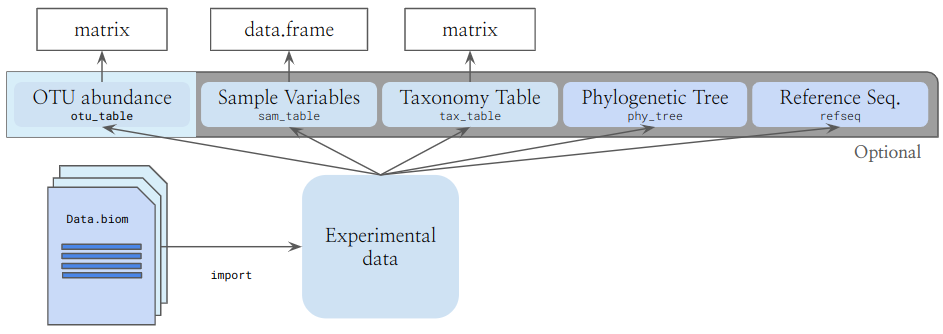
\includegraphics[width=\textwidth]{Img/cap2/Phyloseq.png}
\caption{Estructura del Objeto Phyloseq: Organización Integral de Datos Metagenómicos para Análisis de Diversidad Microbiana, que integra tablas de abundancia, datos taxonómicos, metadatos de las muestras y árboles filogenéticos. Este formato permite un análisis eficiente y completo de las comunidades microbianas.}%\citep{Introducción a phyloseq-castrolab})}
\end{figure}

\subsection{R \& RStudio}
R es un lenguaje de programación y un entorno de software diseñado específicamente para el análisis estadístico y la visualización de datos. Desarrollado inicialmente por Ross Ihaka y Robert Gentleman en 1993, se ha convertido en una herramienta esencial en biología, ecología, genómica y otras disciplinas científicas que requieren análisis cuantitativos. Su principal fortaleza radica en la disponibilidad de bibliotecas especializadas, como ggplot2 para visualización y phyloseq para análisis de microbiomas, además de su comunidad activa, que contribuye con paquetes de código abierto. R se utiliza ampliamente en análisis de datos complejos, modelado estadístico, aprendizaje automático y visualización avanzada, facilitando la reproducibilidad y el manejo de grandes volúmenes de datos.\\

RStudio es un entorno de desarrollo integrado (IDE) diseñado para trabajar con el lenguaje de programación R. Ofrece una interfaz intuitiva que facilita la escritura, ejecución y depuración de código, así como la visualización de resultados. RStudio permite organizar proyectos, gestionar paquetes y bibliotecas, y crear documentos reproducibles con R Markdown. También es compatible con Shiny para aplicaciones interactivas. Disponible en versiones gratuitas y de pago, RStudio es ideal tanto para principiantes como para expertos en análisis de datos.\\

\section{Formatos}

\subsection{JSON}
JSON (JavaScript Object Notation) es un formato de texto ligero para el intercambio de datos estructurados, representado como pares clave-valor u objetos anidados. En bioinformática, se utiliza comúnmente para almacenar metadatos y resultados jerarquizados debido a su compatibilidad con múltiples lenguajes de programación y su facilidad de lectura. Se emplea frecuentemente para guardar información de taxonomía, anotaciones funcionales o resultados de herramientas como QIIME 2, que lo usa para almacenar objetos complejos, como árboles filogenéticos y tablas de abundancia.\\

\subsection{BIOM}
El formato BIOM (Biological Observation Matrix) es un estándar binario utilizado en bioinformática para almacenar matrices de datos biológicos, especialmente en estudios de microbiomas. Facilita el almacenamiento eficiente de datos de abundancia y metadatos asociados, y es compatible con herramientas como QIIME y Phyloseq. El formato contiene tablas de abundancia con taxones como filas, muestras como columnas y valores numéricos que representan abundancias relativas o absolutas. Además, permite incluir metadatos sobre muestras y taxones, como información ambiental o taxonómica.\\

\subsection{FASTA}
FASTA (Fast Alignment Search Tool-All) es un formato de texto plano que almacena secuencias de ADN, ARN o proteínas. Cada entrada contiene un encabezado (precedido por "\>") seguido de una línea con la secuencia biológica. Es ampliamente utilizado para compartir datos genómicos y transcriptómicos.\\

FASTQ es un formato que extiende FASTA, añadiendo información sobre la calidad de cada nucleótido o aminoácido. Es fundamental para los datos generados por plataformas de secuenciación de próxima generación (NGS). Cada entrada en FASTQ tiene cuatro líneas:
\begin{enumerate}
\item Un identificador de la secuencia.
\item La secuencia biológica.
\item Un separador "$+$".
\item Una línea con la puntuación de calidad (en formato ASCII).
\end{enumerate}

\subsection{BAM}
BAM (Binary Alignment/Map) es un formato binario utilizado para almacenar datos de alineamiento de secuencias genómicas. Es una versión comprimida y binaria del formato SAM (Sequence Alignment/Map), que es un formato de texto para almacenar los mismos datos. BAM es ampliamente utilizado en bioinformática, especialmente en análisis de datos de secuenciación de próxima generación (NGS), debido a su eficiencia en el almacenamiento y procesamiento de grandes volúmenes de datos.\\

Cada archivo BAM contiene información detallada sobre cómo las secuencias de ADN se alinean con una referencia genómica, incluyendo la posición de la secuencia en el genoma, la calidad del alineamiento, las secuencias de los nucleótidos y las puntuaciones de calidad. Dado que el formato BAM es binario, es más compacto y rápido de manejar en comparación con su contraparte en texto, SAM.\\

\section{Solena}
Solena es una empresa de biotecnología agrícola (AgTech) enfocada en el análisis y mejora del microbioma del suelo. Su misión es desarrollar soluciones innovadoras basadas en datos moleculares y biotecnología para optimizar la salud del suelo y, como consecuencia, aumentar la productividad agrícola. Aprovechando herramientas avanzadas como inteligencia artificial y genómica, Solena obtiene conocimientos profundos sobre la composición y funcionalidad del microbioma del suelo. Además, en colaboración con organizaciones locales, la empresa implementa centros de diagnóstico molecular agrícola, como el establecido en México, para evaluar la salud de los suelos y fomentar prácticas agrícolas regenerativas.



\section{fresa}

rizosfera 
datos de fresas 
plantas sanasy enfermas 
El estudio investiga las diferencias en la estructura y diversidad de la comunidad microbiana del suelo rizosférico asociadas a plantas de fresa (Fragaria × ananassa) infectadas y no infectadas con el oídio (Podosphaera aphanis). Utilizando tecnología de secuenciación de alto rendimiento (Illumina MiSeq), se analizaron las comunidades microbianas para evaluar los efectos del patógeno sobre la microbiota del suelo en condiciones controladas de invernadero. El objetivo principal fue caracterizar las diferencias en la composición y diversidad microbiana de la rizosfera entre plantas infectadas y no infectadas, explorando posibles relaciones entre la infección por oídio y cambios en el microbioma rizosférico.(yang2020comparison)\\


\section{Simuladores de Secuencias metagenomicas}

CAMISIM es un simulador de secuencias metagenómicas, este software puede simular una amplia variedad de comunidades microbianas y conjuntos de datos metagenomicos, este algoritmo se divide en tres partes, la primera es el diseño de la comunidad, aqui se crean dichos datos a partir de perfiles taxonomicos de novo o de una base de datos genomicos dada (\cite{fritz2019camisim}). Para el diseño a partir de perfiles taxonomicos, se incluye una base de datos de la taxonomia de NCBI (National Center for Biotechnology Information), y se proporcionan en formato BIOM (Biological Observation Matrix format); estos perfiles pueden incluir taxones de bacterias,arqueas y eucariotas asi como virus. Para el diseño de comunidad de novo, se necesitan genomas en formato .fasta y un archivo de mapeo que contenga ID taxonomico (de NCBI) y OTU para cada genoma.  \\

En segunda parte se basa en la simulacion del metagenoma, los conjuntos de datos del metagenoma se generan a partir de los perfiles de abundancia y genomas del paso anterior; las longitudes de los reads y los tamaños de los insertos se pueden variar para algunos simuladores. Para cada conjunto de datos, CAMISIM genera archivos FASTQ y un archivo BAM.  \\

Y por ultimo en la tercera parte se tiene la creación y posprocesamiento de estandares de oro de ensamblaje y agrupacion, a partir de los datos del metagenoma simulado,los archivos FASTQ y BAM. CAMISIM genera los estándares de oro del genoma y el taxón para las lecturas y los contigs ensamblados, respectivamente. Estos especifican el genoma y el linaje taxonómico al que pertenecen las secuencias individuales. Todas las secuencias se pueden anonimizar y mezclar (pero rastrear durante todo el proceso), para permitir su uso en desafíos de evaluación comparativa.  \\

\begin{itemize}
    \item CAMISIM es un programa flexible para simular una gran variedad de comunidades microbianas y muestras de metagenomas. 
    \item Posee un conjunto de funciones completo para simular comunidades microbianas realistas y conjuntos de datos de metagenomas.
    \item Exploraron el efecto de las propiedades específicas de los datos en el rendimiento del ensamblador.
\end{itemize}



DeepMAsED tiene un enfoque de deeplearning para identificar contig  mal ensamblados sin necesidad de genomas de referencia.\\




\thispagestyle{empty}

\chapter{Análisis Exploratorio de Datos}

Un análisis exploratorio se realiza para una investigacion y entendimiento afondo de los datos, y asi descubrir patrones ocultos y generar hipótesis, a traves de tecnicas de visualización de datos, análisis de correlación o minería de datos.\\

El propósito de este análisis es identificar características diferenciadoras entre los microbiomas de plantas sanas y enfermas mediante el uso de datos metagenómicos. Para llevar a cabo este estudio, se obtuvieron datos metagenómicos de la empresa Solena, específicamente de microorganismos presentes en cultivos de fresa. Inicialmente, se dividieron las muestras en dos poblaciones: aquellas etiquetadas como $"$sanas$"$ y $"$enfermas$"$.\\

En una primera etapa, se llevó a cabo un exhaustivo preprocesamiento de los datos, utilizando los lenguajes de programación, BASH y R. Posteriormente, se inició el análisis exploratorio de datos, el cual se estructura principalmente en tres partes. En primer lugar, se realizó una exploración que abarcó las diversidades alfa y beta. Esto condujo a un análisis estadístico respaldado por pruebas de hipótesis. En segundo lugar, se llevó a cabo una visualización de correlaciones mediante redes.\\ %Por último, se implementó una clasificación empleando técnicas de machine learning.\\

Este enfoque integral no solo proporciona una comprensión detallada de la composición de los microbiomas en las plantas de fresa, sino que también permite identificar patrones significativos que podrían ser fundamentales para distinguir entre la salud y la enfermedad en estos cultivos (\cite{yang2020}). 
Este enfoque integral no solo proporciona una comprensión detallada de la composición de los microbiomas en las plantas de fresa, sino que también permite identificar patrones significativos en las diferencias ya sea de presencia-ausencia o abundancia de microorganismos, que podrían ser fundamentales para distinguir entre la salud y la enfermedad en estos cultivos.

\section{Preprocesamiento}

Dentro de las etapas principales de los datos, se encuentra la adquisición de los datos, en donde se recopilan los datos necesarios para el análisis. Se ha adquirido un conjunto de datos metagenómicos de cultivos de fresa proporcionados por Solena. Estas secuencias se entregaron en formato fasta y se encuentran almacenadas en archivos Json, siendo el resultado de la clasificación metagenómica realizada mediante el clasificador Kraken. Con la finalidad de identificar características distintivas entre los frutos sanos y enfermos, hemos llevado a cabo un análisis exploratorio de estos datos.\\

\begin{figure}[h]
\centering
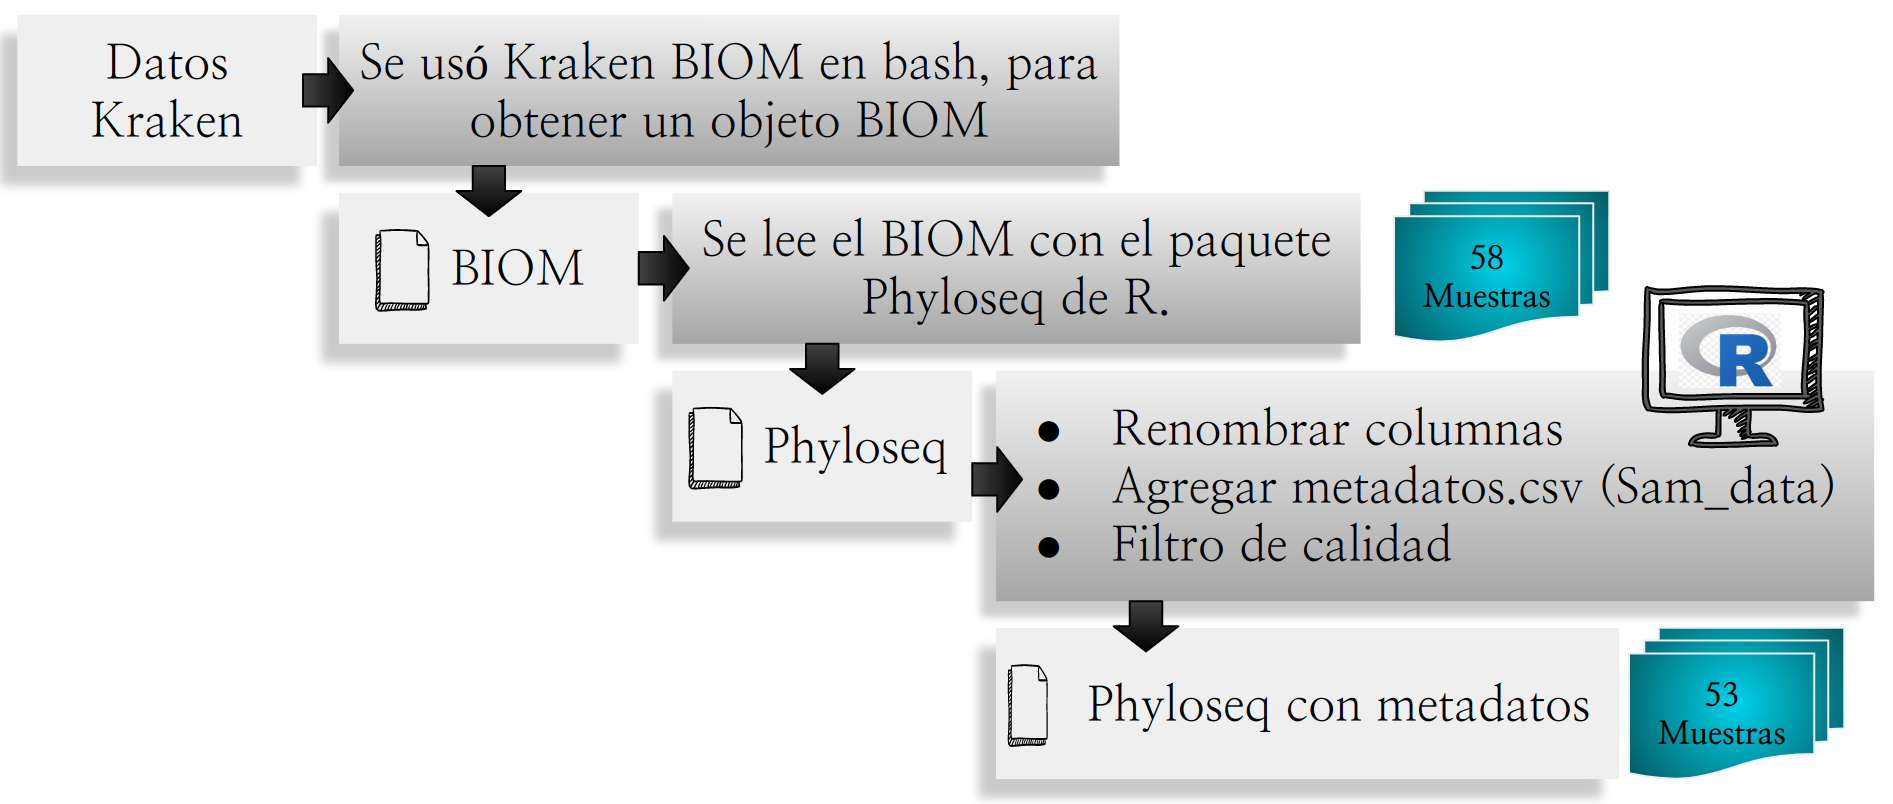
\includegraphics[width=\textwidth]{Img/cap2/preprosecamiento.png}
\caption{Flujo de trabajo, preprocesamiento de datos}
\end{figure}

Dentro de este preprocesamiento es necesario realizar una limpieza y trasformación de los datos para que estos sean adecuados para el análisis. En este caso se realizó un cambio de formato a objeto BIOM, para un mejor manejo de los datos; luego fue necesario renombrar columnas, agregar los metadatos y realizar un filtro de calidad, que se explicara a fondo más adelante.\\

\subsection{Phyloseq}

Phyloseq es un Software de Código Abierto para Bioinformática (Open Source Software For Bioinformatics), diseñado para la manipulación y análisis integral de datos metagenómicos generados mediante tecnologías de secuenciación de alto rendimiento. Esta herramienta en R ofrece capacidades para importar, almacenar, analizar y visualizar datos metagenómicos de manera eficiente. En el entorno de R, estos datos se estructuran en un objeto Phyloseq, el cual tiene la versatilidad de contener elementos clave, como la tabla de taxonomía, la tabla de conteos, la tabla de muestras o metadatos, y el árbol filogenético. Esta organización multifacética facilita un análisis completo y preciso de la estructura de la comunidad microbiana, brindando una comprensión profunda de los datos metagenómicos en cuestión. (\cite{mcmurdie2013})\\

\begin{figure}[h]
\centering
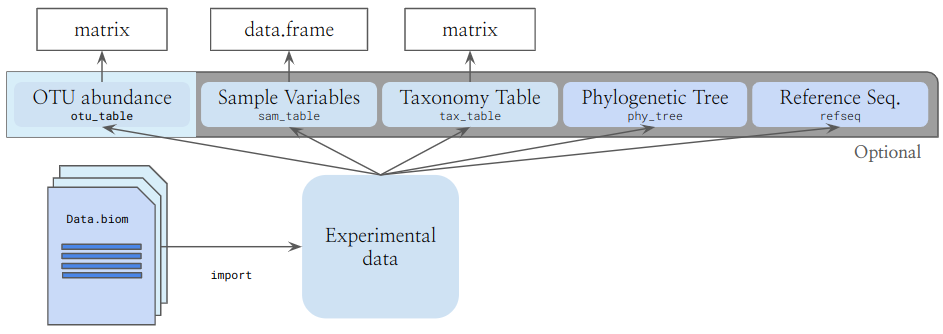
\includegraphics[width=\textwidth]{Img/cap2/Phyloseq.png}
\caption{Objeto phyloseq }%\citep{Introducción a phyloseq-castrolab})}
\end{figure}

Para iniciar el análisis de estos datos, llevamos a cabo una exploración general utilizando índices ecológicos, especialmente centrándonos en las diversidades alfa y beta. Importamos los datos como un objeto Phyloseq, que puede incluir cuatro componentes: la matriz de abundancias, la tabla de taxonomía, los metadatos y el árbol filogenético. Este enfoque nos permite obtener una comprensión más profunda de la estructura de la comunidad microbiana presente en los datos metagenómicos, empleando medidas de diversidad para evaluar la variabilidad intra e inter-muestral.

\subsection{Filtrado de Calidad}

Después de realizar una revisión inicial de los datos, notamos la presencia de muestras con conteos de ceros (número de lecturas por muestras), como en el caso de 'MP2088'. A través de Solena, obtuvimos una tabla que refleja la calidad de las muestras (fastp.kraken.summary \href{https://github.com/CamilaSilva1995/Tesis_Maestria/blob/main/Analisis_Comparativo/Fresa_Solena/01_Exploracion.pdf}). Esta información es crucial para determinar qué muestras pueden ser eliminadas de nuestro conjunto de datos, ya que no cumplen con ciertos estándares de calidad. La identificación y exclusión de muestras que no cumplen con estos criterios contribuirá a asegurar la integridad y la confiabilidad de nuestro dataset, garantizando que solo las muestras de alta calidad sean consideradas en el análisis subsiguiente.\\

Esta tabla proporciona información detallada sobre la calidad de las muestras, destacando diversos parámetros clave:
\begin{itemize}
  \item \textbf{ID de la muestra:} Identificación única de la muestra.
  \item \textbf{Reads\_B  (Reads\_Before):} Número total de lecturas crudas antes del análisis de calidad.
  \item \textbf{Reads\_A (Reads\_After):} Número total de lecturas después del análisis de calidad.
  \item \textbf{Reads\_diff:}  Diferencia entre Reads\_B y Reads\_A.
  \item \textbf{Q30\_B:} Porcentaje de lecturas con calidad superior a 30 (escala fred) antes del análisis de calidad.
  \item \textbf{Q30\_A:} Porcentaje de lecturas con calidad superior a 30 después del análisis de calidad.
  \item \textbf{LowQua:} Lecturas de baja calidad.
  \item \textbf{N\_reads:} Lecturas que contienen 'N' y son descartadas.
  \item \textbf{too\_short:}  Lecturas que no cumplen con el tamaño mínimo de calidad.
  \item \textbf{Duplication:} Porcentaje de duplicados.
  \item \textbf{LengthR1:} Longitud promedio de las lecturas en la muestra.
  \item \textbf{LengthR2:} Longitud promedio de las lecturas en la muestra.
  \item \textbf{Classified:} Porcentaje de lecturas clasificadas del total después del filtrado.
\end{itemize}

Como ejemplo, la muestra MD2055 inicialmente tiene 97 millones de lecturas antes del filtrado, y después del análisis de calidad queda con 79 millones. El criterio para eliminar muestras es que, después del filtrado de calidad, contengan menos de 25 millones de lecturas. Bajo este filtro, se identificaron y eliminaron cinco muestras: MP2079, MP2080, MP2088, MP2109, MP2137.\\

Eliminamos las muestras de baja calidad, usando el filtro de menos de 25 millones de lecturas luego del análisis de calidad.\\

Este enfoque de eliminación se basa en mantener un umbral mínimo de calidad, contribuyendo así a garantizar la robustez y confiabilidad de las muestras seleccionadas para análisis subsiguientes. Además, se puede realizar un recuento de lecturas por muestra para evaluar la calidad relativa entre las diferentes muestras,\\

\begin{lstlisting}[basicstyle=\small] 
sample_sums(fresa_kraken)
\end{lstlisting}

\resizebox{0.9\textwidth}{!} {
\begin{tabular}{ c c c c c c c c }
MD2055 & MD2056 & MD2065 & MD2066 & MD2075 & MD2076 & MD2085 & MD2086 \\
9782432 & 12468526 & 11297600 & 15580959 & 12310781 & 16067839 & 10524919 & 9931297 \\
MD2095 & MD2096 & MD2105 & MD2106 & MD2115 & MD2116 & MD2125 & MD2126 \\
18009912 & 14998268 & 11792397 & 4053295 & 13102554 & 12451637 & 8355853 & 14307309 \\
MD2135 & MD2136 & MP2047 & MP2048 & MP2049 & MP2050 & MP2057 & MP2058 \\
7280751 & 6172369 & 9199079 & 12146967 & 13075806 & 16098757 & 17141427 & 20923502 \\
MP2059 & MP2060 & MP2067 & MP2068 & MP2069 & MP2070 & MP2077 & MP2078 \\
14129981 & 13786630 & 16924218 & 20873789 & 15537530 & 12462356 & 9617847 & 7588787 \\
MP2079 & MP2080 & MP2087 & MP2088 & MP2089 & MP2090 & MP2097 & MP2098 \\
745830 & 3125701 & 20632320 & 2 & 16582404 & 11176782 & 11714000 & 16595897 \\
MP2099 & MP2100 & MP2107 & MP2108 & MP2109 & MP2110 & MP2117 & MP2118 \\
14844038 & 13342326 & 11014462 & 6728020 & 1405462 & 6901265 & 12624002 & 14711376 \\
MP2119 & MP2120 & MP2127 & MP2128 & MP2129 & MP2130 & MP2137 & MP2138 \\
9835326 & 10975712 & 7106567 & 9974861 & 8348307 & 6196725 & 2169734 & 8220431 \\
MP2139 & MP2140 \\
6158581 & 5267510
\end{tabular}
}

La muestra MP2088 plantea un desafío evidente al contener solo 2 lecturas. Esta escasez de datos representa un problema significativo durante el análisis, ya que la falta de información sustancial puede afectar la validez y la interpretación de los resultados. Por lo tanto, esta muestra fue eliminada utilizando el filtro de calidad establecido, que se basa en mantener muestras con un número mínimo de lecturas después del análisis.\\

La eliminación de muestras con un conteo tan bajo es crucial para garantizar la integridad y la confiabilidad de los resultados del análisis. Al eliminar muestras con datos insuficientes, se mejora la calidad general del conjunto de datos y se evitan posibles distorsiones o sesgos que podrían surgir debido a la falta de información significativa.\\

Este enfoque de eliminación selectiva respalda la robustez del análisis de datos metagenómicos, permitiendo una interpretación más precisa y confiable de la diversidad microbiana en las muestras restantes.\\

\begin{lstlisting}[basicstyle=\small] 
sample_sums(fresa_kraken_fil)
\end{lstlisting}

\resizebox{0.9\textwidth}{!} {
\begin{tabular}{ c c c c c c c c }
MD2055 & MD2056 & MD2065 & MD2066 & MD2075 & MD2076 & MD2085 & MD2086 \\
9782432 & 12468526 & 11297600 & 15580959 & 12310781 & 16067839 & 10524919 & 9931297 \\
MD2095 & MD2096 & MD2105 & MD2106 & MD2115 & MD2116 & MD2125 & MD2126 \\
18009912 & 14998268 & 11792397 & 4053295 & 13102554 & 12451637 & 8355853 & 14307309 \\
MD2135 & MD2136 & MP2047 & MP2048 & MP2049 & MP2050 & MP2057 & MP2058 \\
7280751 & 6172369 & 9199079 & 12146967 & 13075806 & 16098757 & 17141427 & 20923502 \\
MP2059 & MP2060 & MP2067 & MP2068 & MP2069 & MP2070 & MP2077 & MP2078 \\
14129981 & 13786630 & 16924218 & 20873789 & 15537530 & 12462356 & 9617847 & 7588787 \\
MP2087 & MP2089 & MP2090 & MP2097 & MP2098 & MP2099 & MP2100 & MP2107 \\
20632320 & 16582404 & 11176782 & 11714000 & 16595897 & 14844038 & 13342326 & 11014462 \\
MP2108 & MP2110 & MP2117 & MP2118 & MP2119 & MP2120 & MP2127 & MP2128 \\
6728020 & 6901265 & 12624002 & 14711376 & 9835326 & 10975712 & 7106567 & 9974861 \\
MP2129 & MP2130 & MP2138 & MP2139 & MP2140 \\
8348307 & 6196725 & 8220431 & 6158581 & 5267510
\end{tabular}
}

\section{Índices de diversidad}

Un índice de diversidad constituye una medida numérica empleada para cuantificar la variedad y la distribución de especies en una comunidad biológica o un ecosistema. Estos índices son herramientas matemáticas diseñadas para sintetizar y comparar la composición de especies en diversas comunidades.\\

El propósito fundamental de los índices de diversidad es proporcionar una manera objetiva y cuantitativa de comprender la estructura y la abundancia relativa de las especies en el seno de una población o comunidad biológica. En este contexto, iniciaremos un análisis de diversidad de nuestras muestras, empleando dos métricas fundamentales: la Diversidad Alfa y la Diversidad Beta (\cite{tuomisto2010}). Estas métricas nos permitirán explorar y comprender tanto la variabilidad interna de una sola comunidad como las diferencias entre varias comunidades, respectivamente.\\ 


\subsection{Diversidad Alfa}

La diversidad alfa, en esencia, refleja la riqueza de las muestras, es decir, el número de especies distintas presentes en un determinado entorno, o la abundancia relativa de dichas especies en dicho entorno; es usada principalmente para medir la diversidad local, haciendo referencia a la diversidad dentro de una muestra o comunidad % (\cite{whittaker1960} & \cite{whittaker1972})
 Para cuantificar esta diversidad, se recurre a diversos índices de medida, cada uno con enfoques particulares.\\

En nuestro análisis de diversidad alfa, consideramos tres índices específicos: Chao1, Shannon y Simpson. El índice Chao1 es una m,edida cualitativa basada en especies
% (\cite{chao1984} & \cite{chao1987}), 
la cual estima el número total de especies presentes en una muestra o comunidad. Por otro lado, el índice Shannon toma en cuenta tanto la riqueza en especies como su abundancia (\cite{shannon1948}), utilizando una escala logarítmica para proporcionar una visión integral de la diversidad. Finalmente, el índice Simpson se centra en la medida de dominancia, otorgando un peso considerable a las especies comunes en comparación con las especies más raras. Siendo estas dos medidas cuantitativas (\cite{simpson1949}).\\

Esta selección de índices nos permite capturar diferentes aspectos de la diversidad alfa, brindando una comprensión más completa de la estructura y la composición de especies en nuestras muestras o comunidades.\\

\textbf{Chao1}, es una métrica que evalúa la riqueza de especies, proporcionando una estimación del número total de especies en una comunidad. Su utilidad se destaca especialmente en situaciones donde la muestra es pequeña o la proporción de especies raras es considerable. Este índice demuestra ser menos sensible a la presencia de especies raras en comparación con otros índices, lo que lo convierte en una herramienta valiosa en estudios centrados en la conservación de especies poco comunes.

La fórmula para calcular el índice Chao1 es la siguiente:
$$S_{Chao1} = S_{Obs} + \frac{F_1×(F_1-1)}{F_2×(F_2+1)}$$
Donde:
\begin{itemize}
    \item $S_{Obs}$ es el número de especies observadas.
    \item $F_1$ es el recuento de "singletons" (especies con un solo individuo en todo el inventario).
    \item $F_2$ es el recuento de "doubletons" (especies con dos individuos en todo el inventario).
\end{itemize}

Esta expresión nos proporciona una estimación más completa de la riqueza de especies al considerar las especies raras representadas por singletons y doubletons. En consecuencia, Chao1 emerge como una herramienta valiosa para evaluar y comparar la diversidad de especies en comunidades biológicas, especialmente en situaciones donde la muestra es limitada o las especies raras desempeñan un papel significativo.\\

El índice de \textbf{Shannon}, representado por $D_{SH}$, es una medida que estima la diversidad de especies, teniendo en cuenta tanto la abundancia como la uniformidad de las especies en una comunidad. Este índice se enfoca en medir la incertidumbre asociada con la identificación de una especie seleccionada al azar en la comunidad. Cuanto mayor sea el índice de Shannon, mayor será la diversidad de especies en la comunidad.

La fórmula para calcular el índice de Shannon es la siguiente:
$$H=-\sum_{i_1}^{S}{P_{i}\ln(P_{i})}$$
Donde:
\begin{itemize}
    \item $S$ es el número de OTU's (Operational Taxonomic Units).
    \item $P_i$ es la proporción de la comunidad representada por $OTU_i$.
\end{itemize}

Esta expresión matemática nos proporciona una medida cuantitativa de la diversidad de especies, tomando en cuenta la riqueza y la uniformidad de las mismas en la comunidad. Un índice de Shannon más alto indica una mayor diversidad, lo que sugiere una distribución más equitativa de abundancias entre las especies presentes. Es decir, comunidades con índices de Shannon más elevados tienden a tener una mayor variedad de especies y una distribución más equilibrada de individuos entre esas especies.\\

\textbf{Simpson}, es una medida de la dominancia relativa de una o unas pocas especies en una comunidad. Este índice evalúa la probabilidad de que dos individuos seleccionados al azar pertenezcan a la misma especie. En términos prácticos, un índice de Simpson más bajo indica una mayor diversidad de especies en la comunidad, lo que sugiere una distribución más equitativa de la abundancia entre las especies presentes.

La fórmula para calcular el índice de Simpson es la siguiente:
$$D=\frac{1}{\sum_{i_1}^{S}{P_{i}^{2}}}$$
Donde:
\begin{itemize}
    \item $S$ en el número total de especies en la comunidad.
    \item $P_i$ es la proporción de la comunidad representada por $OTU_i$.
\end{itemize}

Esta expresión matemática nos proporciona un indicador cuantitativo de la diversidad de especies, donde un índice de Simpson más bajo refleja una comunidad con una mayor variedad de especies y una distribución más uniforme de individuos entre esas especies.\\

En el contexto de la diversidad alfa, estos índices nos permiten explorar y comparar la diversidad de especies en cada muestra o subconjunto, como el grupo de muestras sanas y enfermas. Proporcionan una visión detallada de cómo se distribuye la diversidad de especies dentro de cada conjunto, permitiendo evaluaciones comparativas entre diferentes conjuntos o condiciones.\\

\begin{figure}[h]
\centering
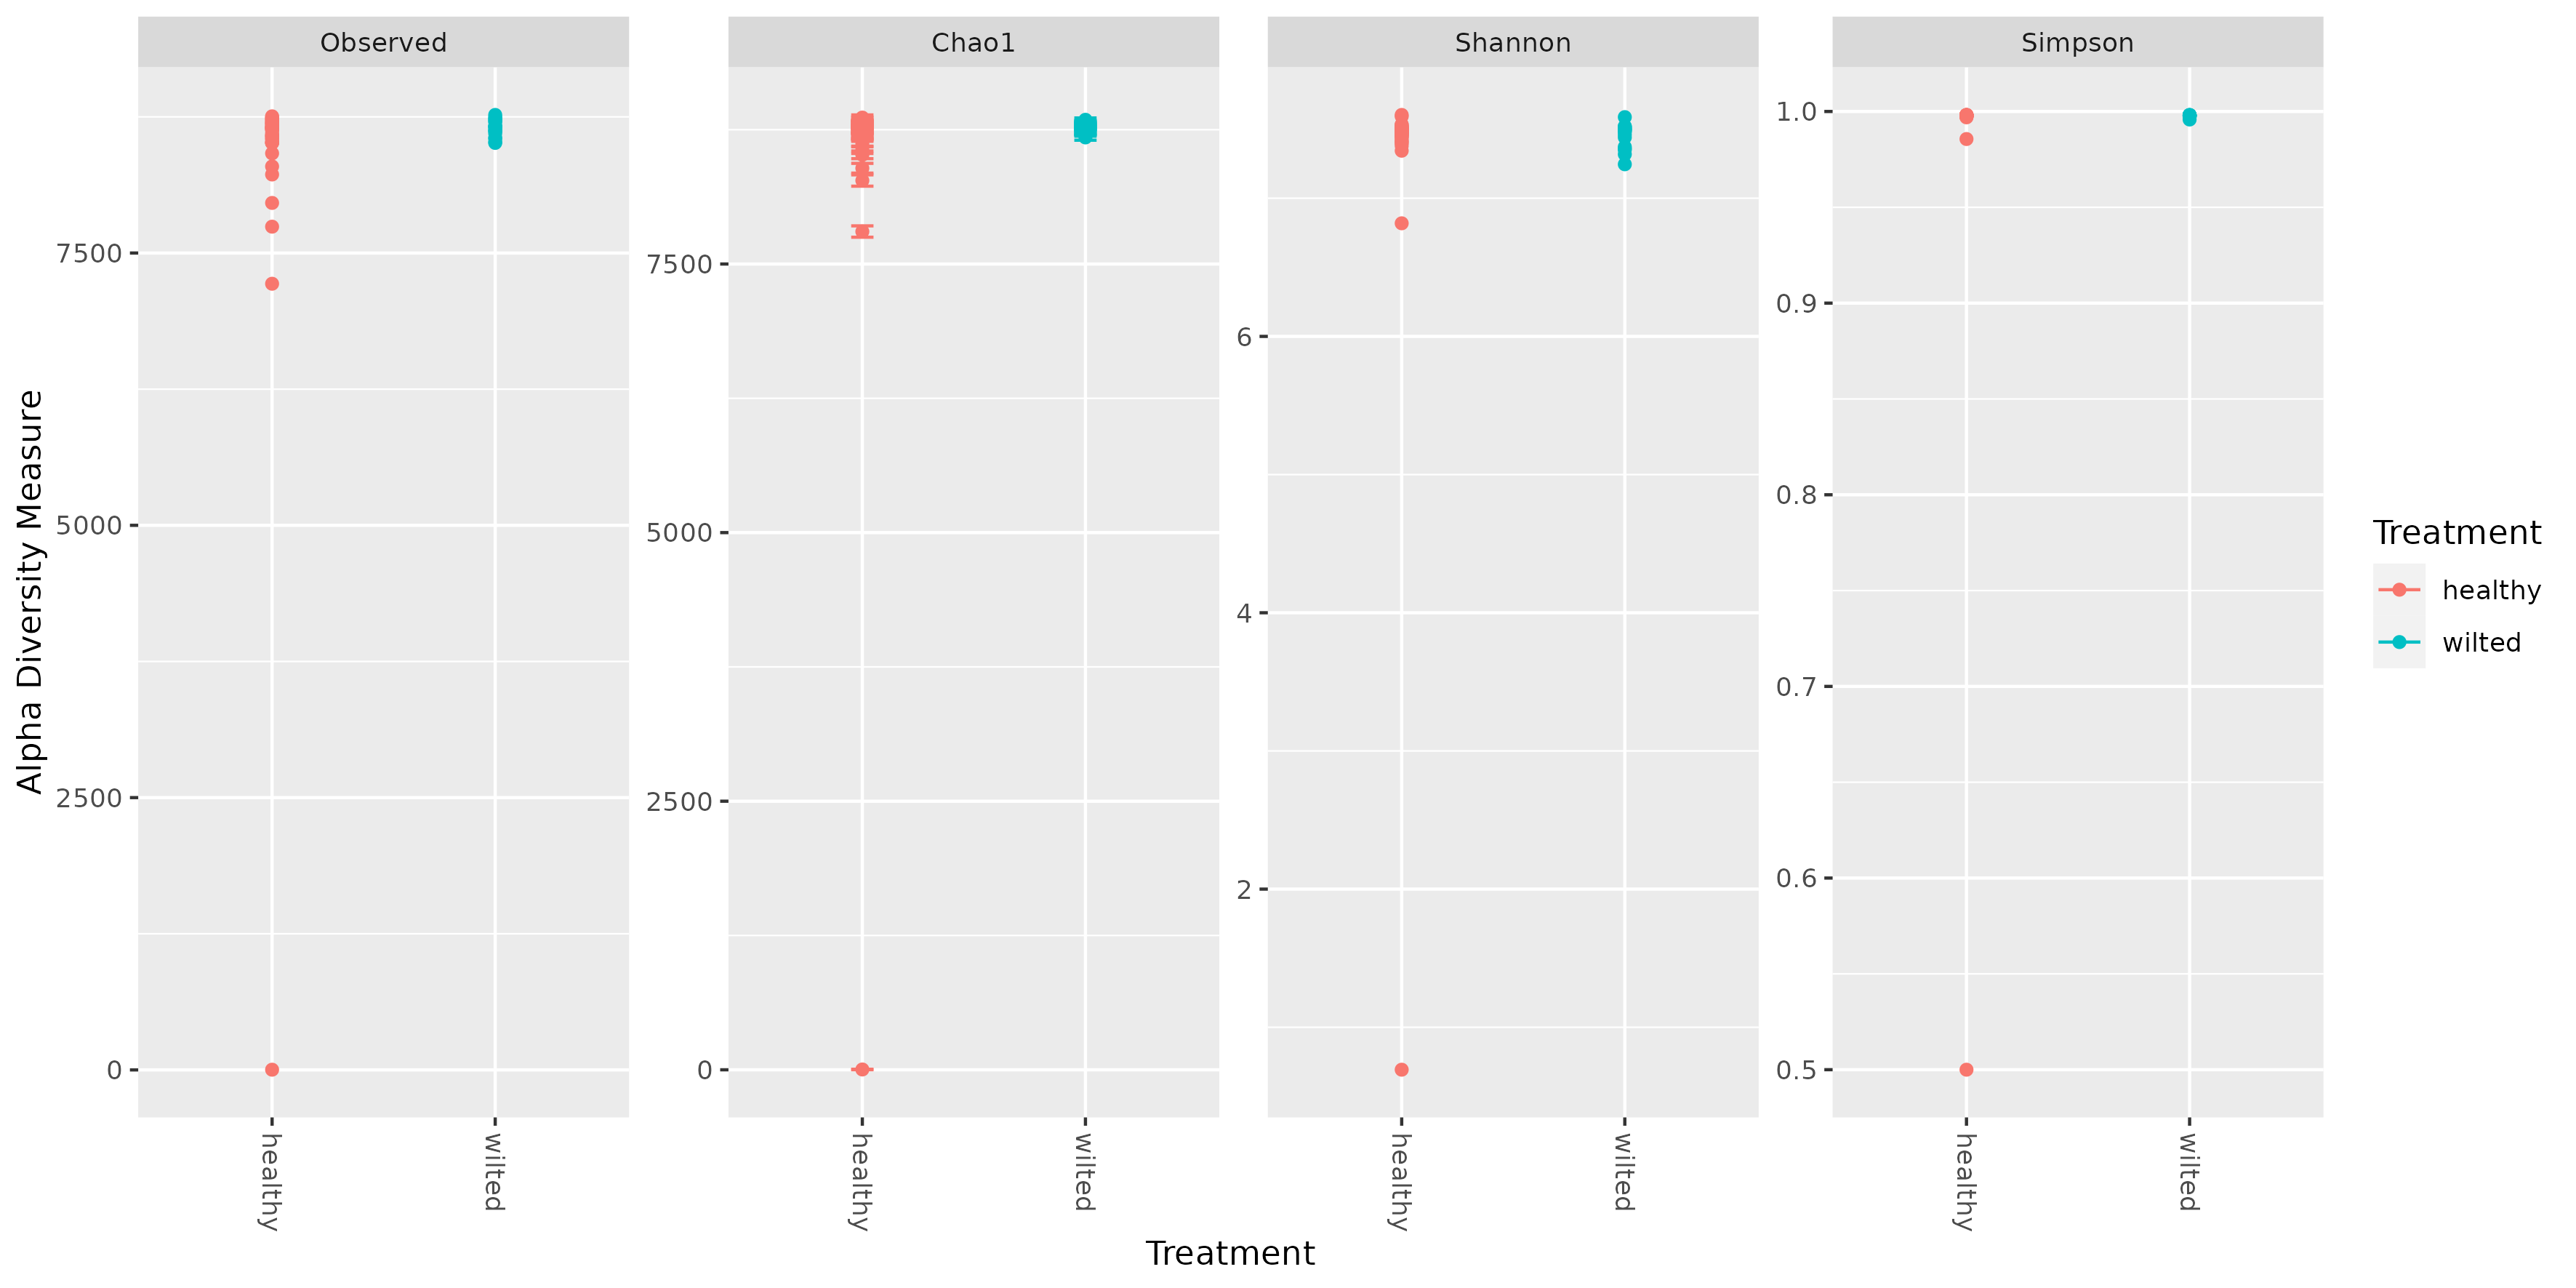
\includegraphics[width=\textwidth]{Img/cap2/DiversidadAlfaFresaKraken.png}
\caption{Diversidad alfa datos crudos metagenomicos de fresa, \href{https://github.com/CamilaSilva1995/Tesis_Maestria/blob/main/Analisis_Comparativo/Fresa_Solena/01_Exploracion.Rmd}{(Exploracion.Rmd)} }
\end{figure}

En la imagen, se pueden identificar datos no deseados que afectan la visualización, por lo que se lleva a cabo un filtro de calidad de los datos.\\

Eliminar muestras de baja calidad resulta en una mejora significativa en la claridad y la interpretación de la visualización. La diferencia es notable después de descartar las muestras de baja calidad, lo que resalta la importancia de un proceso riguroso de filtrado para obtener resultados más precisos y confiables. Este enfoque contribuye a una representación más fiel de los datos, permitiendo una interpretación más precisa y una toma de decisiones informada.\\

\begin{figure}[h]
\centering
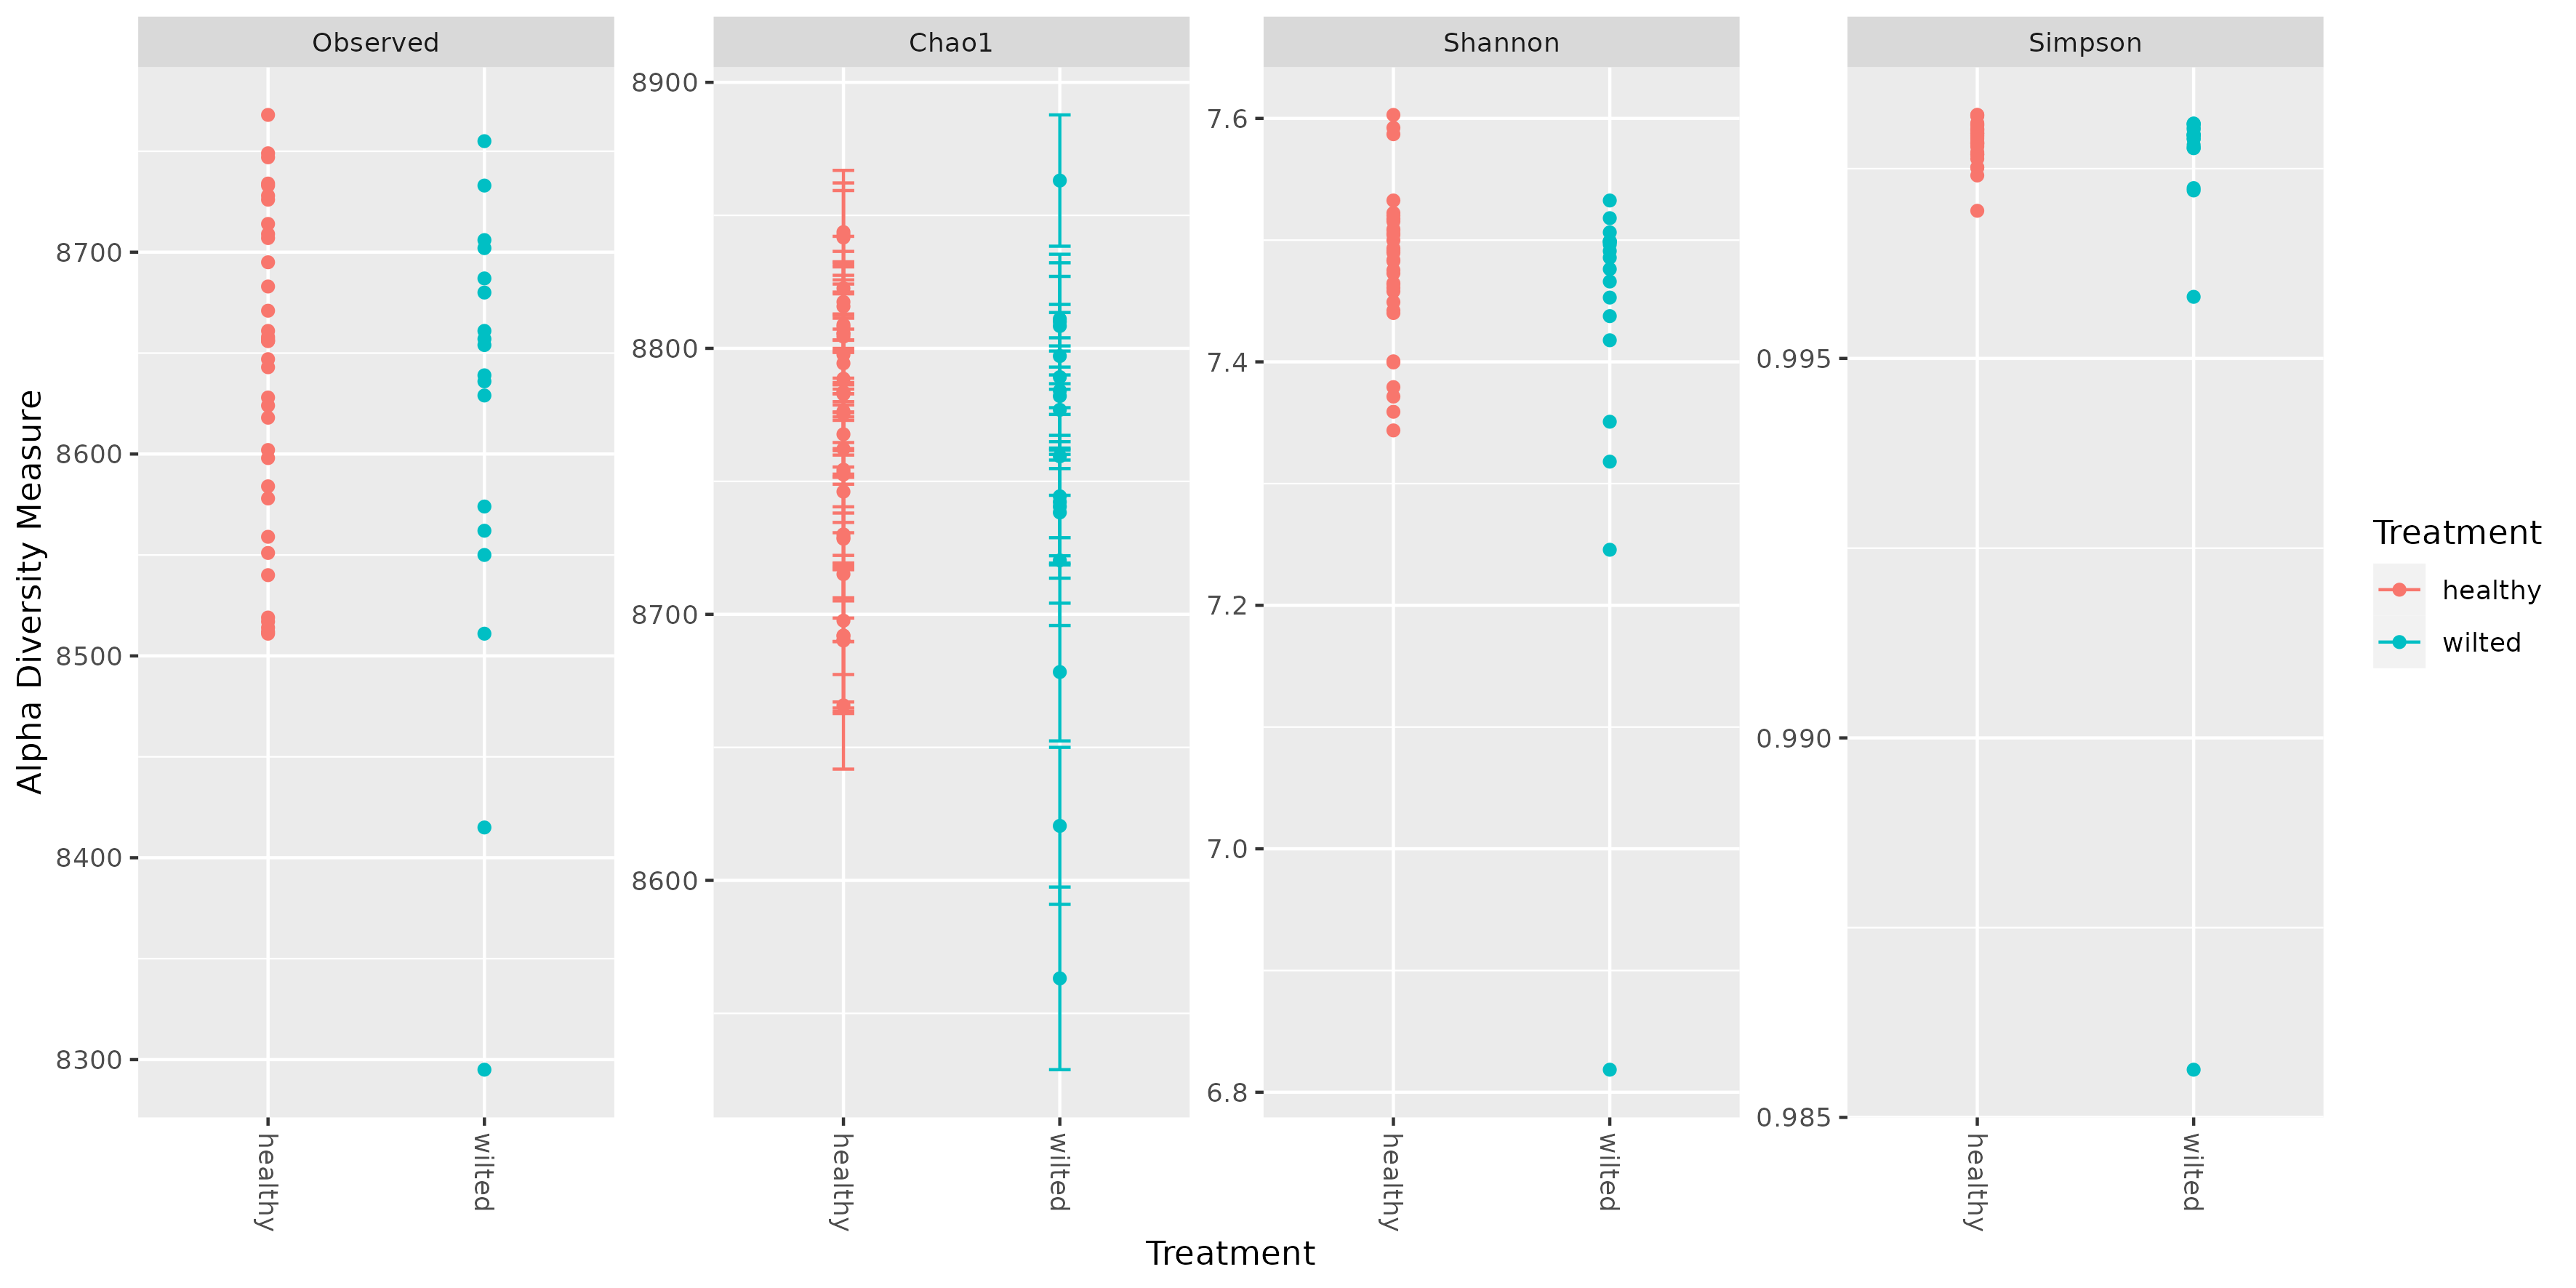
\includegraphics[width=\textwidth]{Img/cap2/DiversidadAlfaFresaKraken_fil.png}
\caption{Diversidad alfa datos filtrados metagenomicos de fresa, \href{https://github.com/CamilaSilva1995/Tesis_Maestria/blob/main/Analisis_Comparativo/Fresa_Solena/01_Exploracion.Rmd}{(Exploracion.Rmd)} }
\end{figure}

Después de aplicar el filtro de calidad de los datos, la visualización de la diversidad alfa en los conjuntos de muestras de plantas sanas y enfermas revela una mayor diversidad en las muestras sanas en comparación con las muestras enfermas. Esta observación se confirma mediante la métrica Chao1, que elimina la influencia de los singletons y doubletons, respaldando la percepción visual de una mayor diversidad en las muestras sanas. A pesar de la diferencia en las diversidades observadas, cabe destacar que esta disparidad no es significativamente grande, sugiriendo que no hay una diferencia sustancial en la diversidad entre las muestras sanas y enfermas.\\

Este análisis proporciona una evaluación más completa de la diversidad alfa, indicando que aunque hay variaciones discernibles, estas no son lo suficientemente notables como para afirmar una gran disparidad en la diversidad entre los conjuntos de muestras. Este tipo de conclusiones respaldadas por métricas específicas y visualizaciones contribuyen a una interpretación más precisa de la composición de las comunidades microbianas en plantas sanas y enfermas\\

\subsection{Diversidad Beta}
La diversidad beta se encarga de evaluar cuán similares o diferentes son un par de especies, muestras, conjuntos de muestras o poblaciones entre sí. Fue definida por Whittaker como una medida del cambio de diversidad a traves de gradientes ambientales, en otras palabras "tasa de cambio en la composisión de especies de una comunidad a otra a los largo de gradientes" (\cite{whittaker1960}). Para medir esta diversidad, se utilizan métricas como la disimilitud de Bray-Curtis, la distancia Jaccard o la distancia UniFrac.\\

Antes de realizar análisis de diversidad beta, es crucial convertir las abundancias absolutas (número de lecturas por OTU) a relativas (porcentajes de lecturas asignadas a un OTU dentro de una muestra). Esta transformación es esencial debido a que los metagenomas tienen tamaños diferentes. Se lleva a cabo el cálculo de las abundancias relativas utilizando la función 'transform\_sample' de Phyloseq, tanto para los datos originales como para los datos filtrados.\\

Este paso es fundamental para garantizar una comparación y evaluación adecuada de la diversidad beta, ya que las abundancias relativas proporcionan una representación más precisa de la estructura de la comunidad, independientemente de las diferencias en el tamaño del metagenoma entre las muestras.\\

\begin{lstlisting}[basicstyle=\small] 
transform_sample_counts(fresa_kraken_fil,
function(x) x*100/sum(x) )
\end{lstlisting}

Usamos “ordinate” para asignar las distancias entre muestras, iniciando y tomando como referencia “Bray-Curtis”, ya que es una de las
metricas mas completas y mayormente utilizadas para medir la diversidad beta.\\

Para visualizar y presentar los resultados de este análisis, se opta por el uso de NMDS (Non-metric Multidimensional Scaling), una herramienta de análisis exploratorio de datos que se emplea para visualizar la similitud o disimilitud entre una colección de objetos (por ejemplo, especies, sitios, genes) en un espacio de baja dimensionalidad. Entre otros, se utilizan ampliamente los análisis PCA, PCoA o NMDS.\\

A continuación, se presenta una lista de distancias disponibles que Phyloseq puede utilizar, siendo las siguientes las más comúnmente utilizadas:\\

La \textbf{Disimilitud de Bray-Curtis}es un índice que se fundamenta en la composición y abundancia de especies en diferentes sitios (\cite{bray&curtis1957}). Este índice mide la similitud entre dos muestras o poblaciones en términos de las especies que comparten, considerando la ponderación de la abundancia de cada especie en cada población.

La fórmula del índice de disimilitud de Bray-Curtis es:
$$d_{BC} = 1 - \frac{2S}{(S_{a} + S_{b})}$$
donde $d_{BC}$ es el índice de disimilitud de Bray-Curtis, $S$ es el número de especies compartidas entre las poblaciones $a$ y $b$, y $S_{a}$ y $S_{b}$ son los números de especies exclusivas de los sitios $a$ y $b$, respectivamente.\\

Este índice proporciona una medida cuantitativa de la diferencia relativa en términos de composición de especies y abundancia entre dos poblaciones o muestras. Cuanto más cercano a 1 sea el valor del índice, mayor será la disimilitud entre las poblaciones.\\

\begin{figure}[h]
\centering
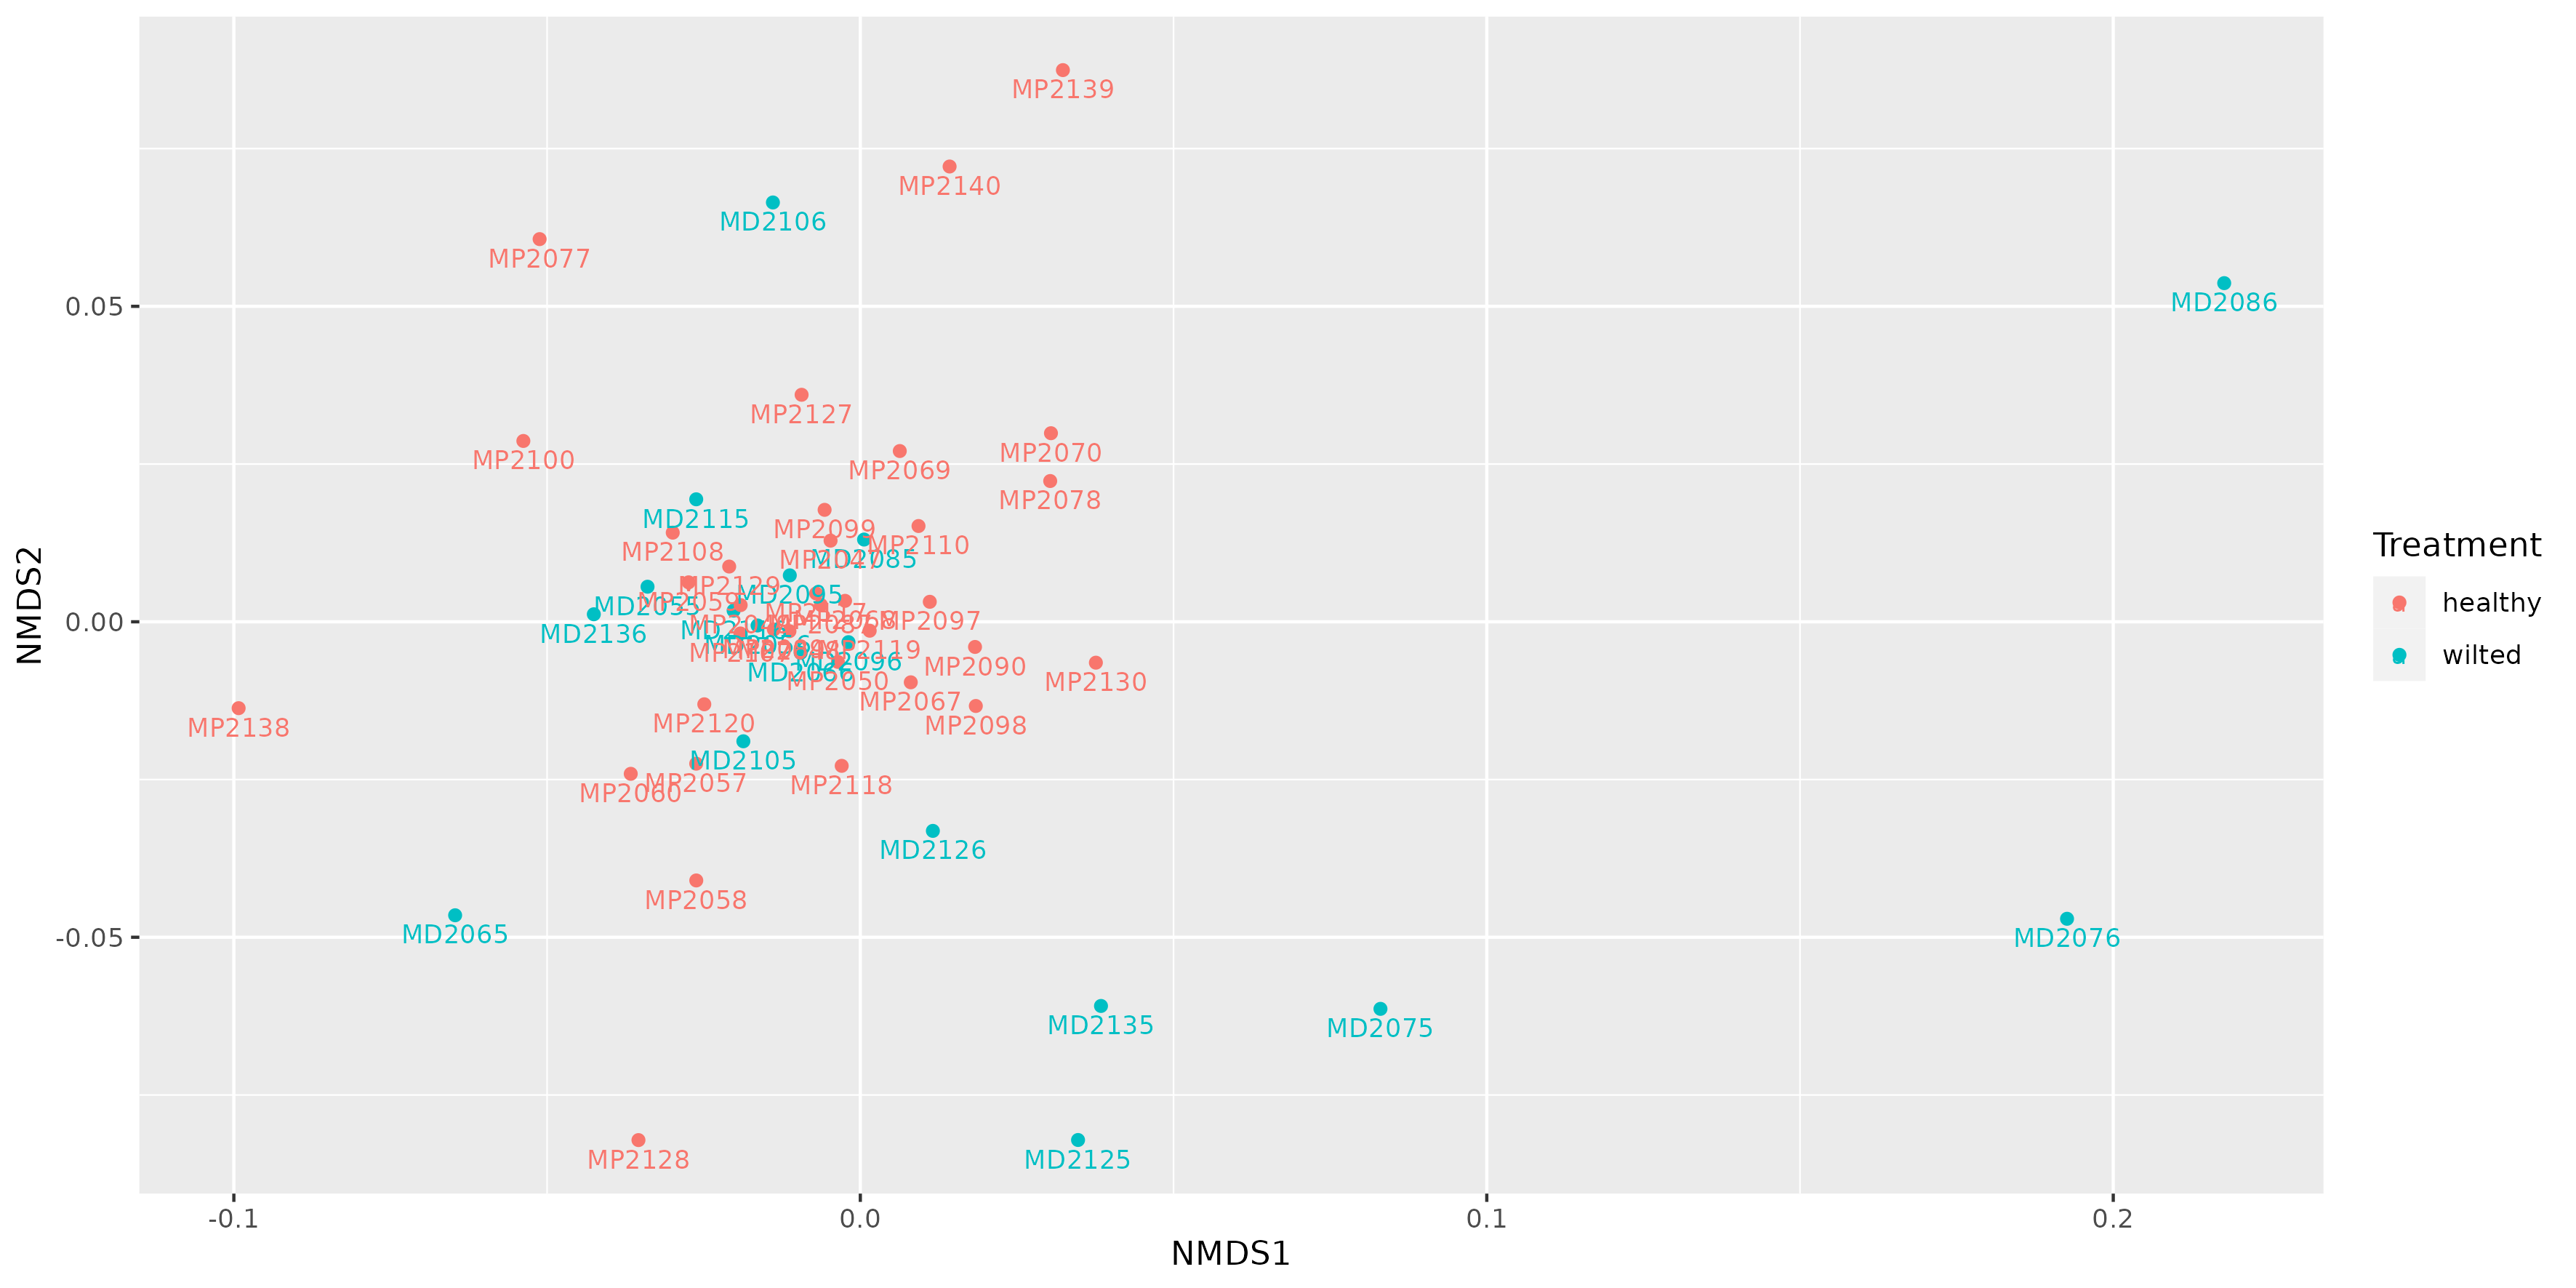
\includegraphics[width=\textwidth]{Img/cap2/DiversidadBetaFresaKraken_fil.png}
\caption{Diversidad Beta, disimilitud de Bray-Curtis,  \href{https://github.com/CamilaSilva1995/Tesis_Maestria/blob/main/Analisis_Comparativo/Fresa_Solena/01_Exploracion.Rmd}{(Exploracion.Rmd)}}
\end{figure}

La \textbf{Distancia Jaccard} es un índice de disimilitud que se basa en la presencia o ausencia de especies en diferentes poblaciones. Este índice compara la proporción de especies que son comunes entre dos poblaciones en relación con el total de especies encontradas en ambas poblaciones. Resulta útil para comparar la diversidad de especies entre diferentes poblaciones o evaluar la similitud en la composición de especies entre comunidades diversas.

La fórmula para el índice de disimilitud de Jaccard es la siguiente:
$$d_{JC} = 1 - \frac{S}{(S_{a} + S_{b}-S)}$$
donde $d_{JC}$ es el índice de disimilitud de Jaccard, $S$ es el número de especies compartidas entre las poblaciones $a$ y $b$, y $S_{a}$ y $S_{b}$ son los números de especies exclusivas de los sitios $a$ y $b$, respectivamente.\\

Este índice ofrece una medida de disimilitud que se centra en la presencia o ausencia de especies, siendo 0 cuando las poblaciones comparten todas las especies y 1 cuando no comparten ninguna. Es especialmente útil para análisis comparativos de la composición de especies entre diferentes comunidades.\\

\begin{figure}[!]
\centering
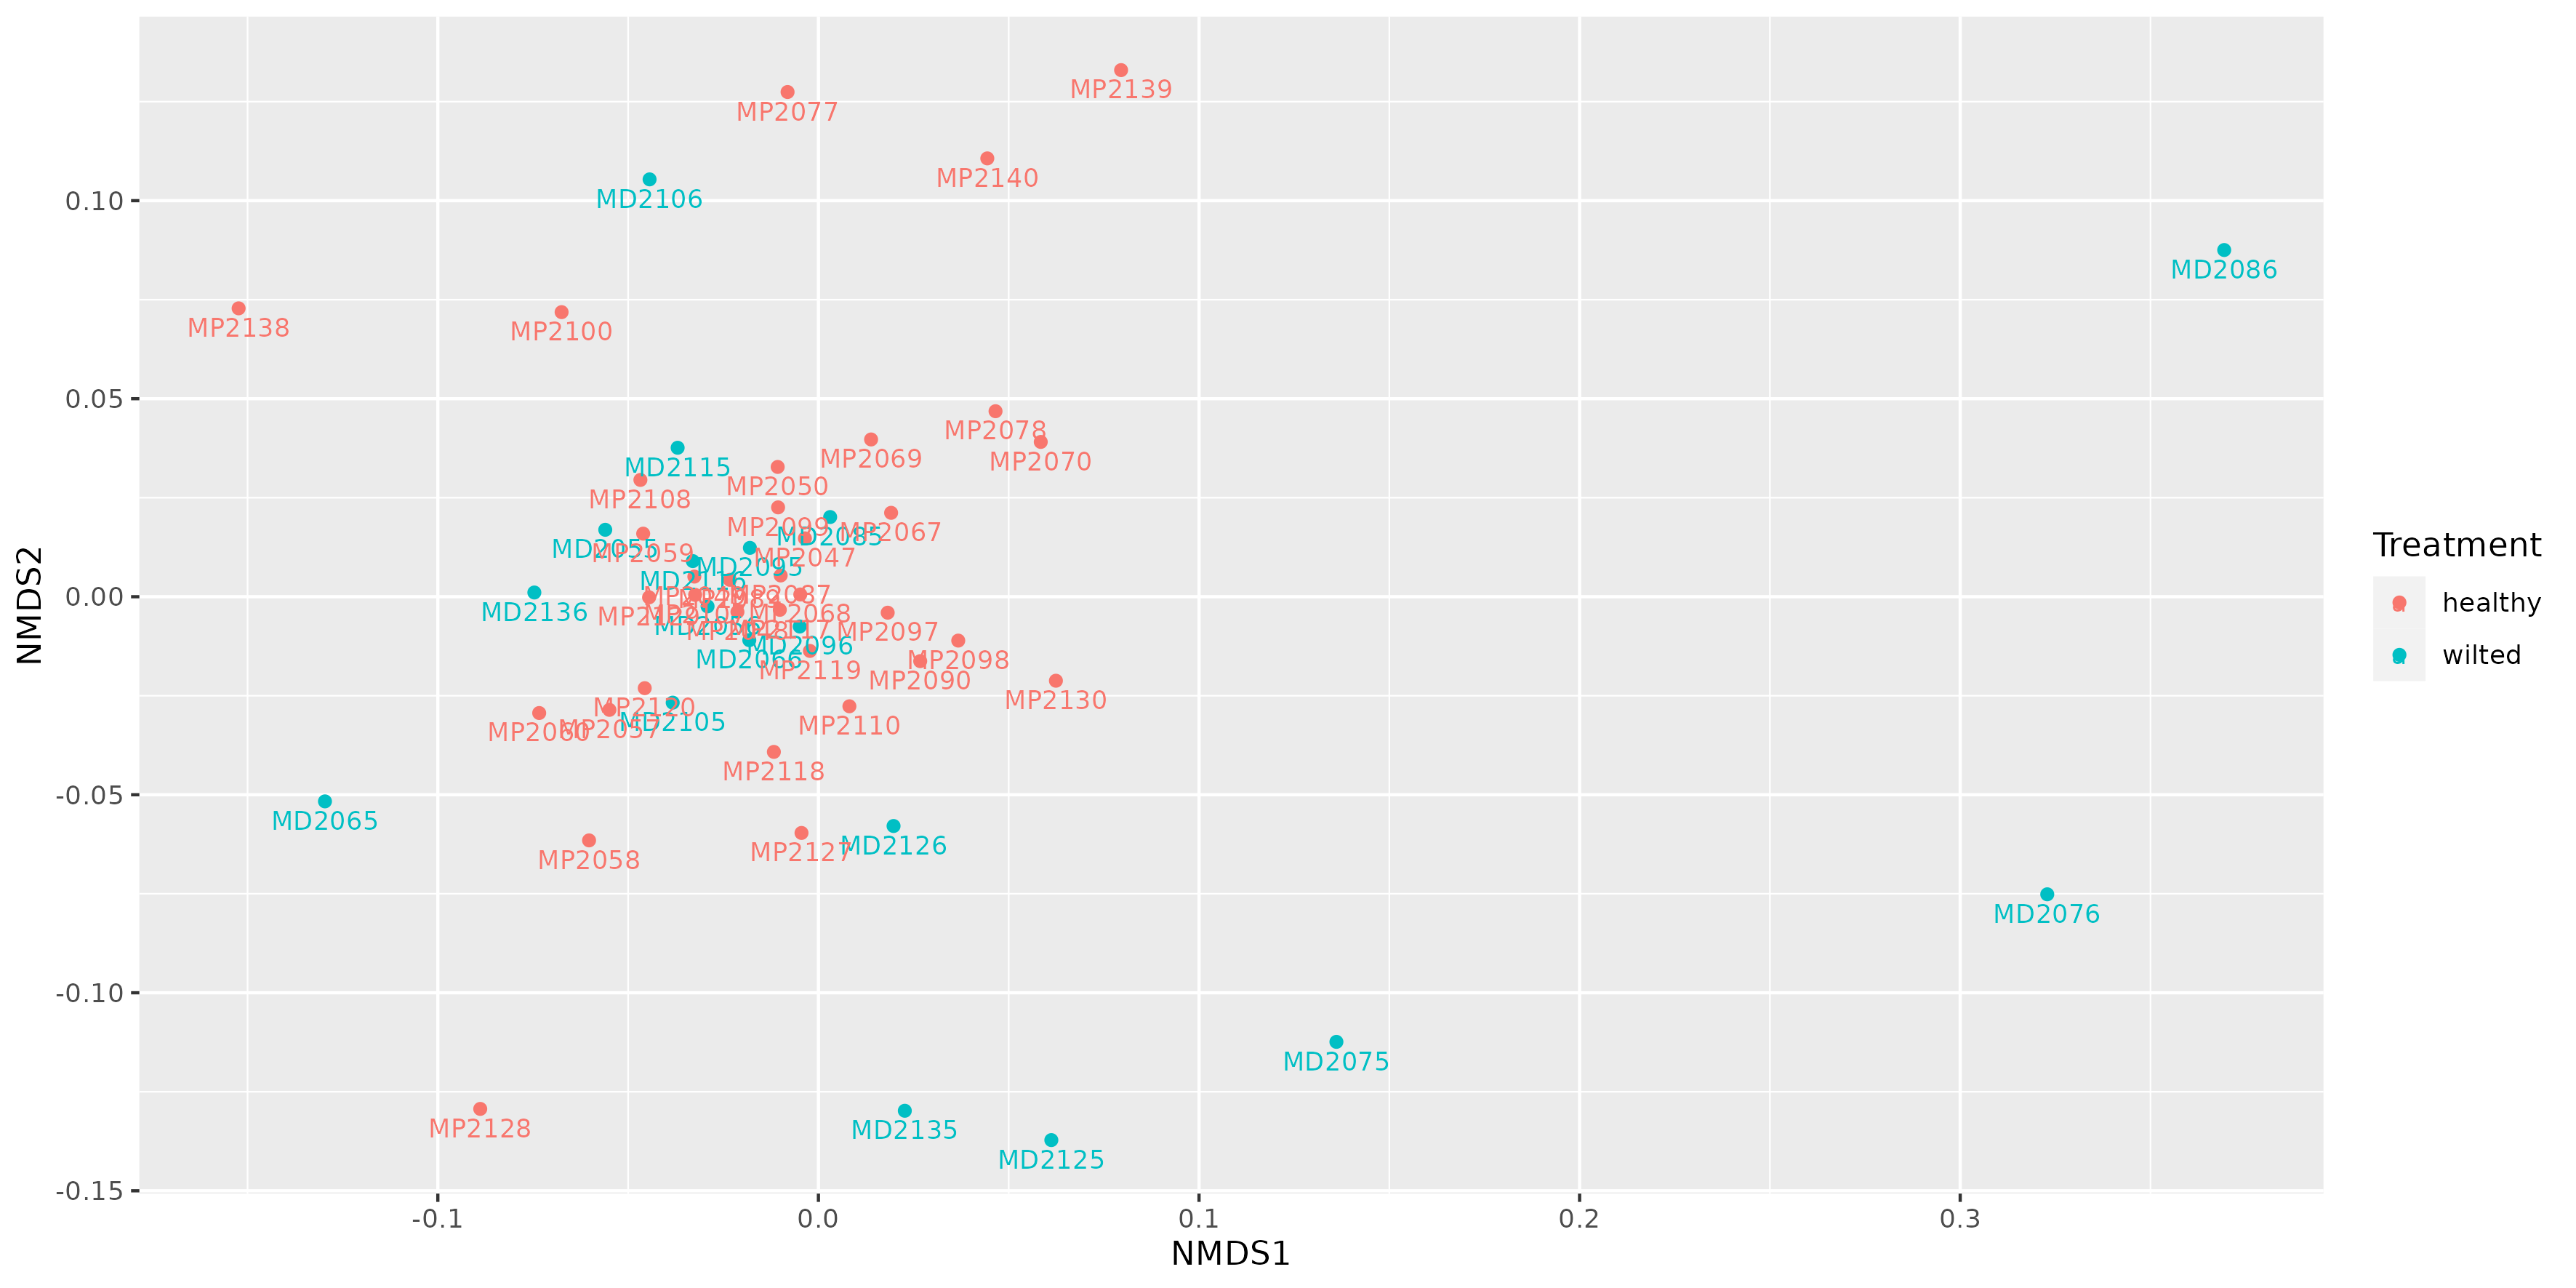
\includegraphics[width=\textwidth]{Img/cap2/DiversidadBetaFresaKraken_fil_jaccard.png}
\caption{Diversidad Beta, distancia de Jaccard, \href{https://github.com/CamilaSilva1995/Tesis_Maestria/blob/main/Analisis_Comparativo/Fresa_Solena/01_Exploracion.Rmd}{(Exploracion.Rmd)}}
\end{figure}

Tomando los datos con filtro de calidad y utilizando la distancia de Jaccard, la cual es la más comúnmente utilizada en este tipo de estudios, se observa que las muestras, tanto sanas como enfermas, están bastante mezcladas. Ante esta observación, se procede a realizar pruebas con distintas distancias para explorar si alguna otra métrica puede proporcionar una separación más clara o revelar patrones específicos en la composición de especies entre las muestras.\\

La distancia \textbf{Euclideana}es comúnmente utilizada en el análisis de datos numéricos y se fundamenta en la diferencia de las abundancias o proporciones de diferentes especies en distintas muestras. Esta distancia mide la separación entre dos muestras como la raíz cuadrada de la suma de las diferencias cuadráticas entre las proporciones de cada especie en ambas muestras.

La fórmula para la distancia Euclidiana entre dos muestras $A$ y $B$ es la siguiente:
$$d_{euclidean} (A,B) = \sqrt{\sum(A_i - B_i)^2}$$
Donde $A_i$ y $B_i$ son las abundancias o proporciones de la especie $i$ en las muestras $A$ y $B$, respectivamente.\\

La distancia Euclidiana es simétrica y cumple con la desigualdad del triángulo, lo que significa que satisface las propiedades de una verdadera distancia. Esta métrica es especialmente adecuada para comparar muestras en términos de diferencias numéricas en las abundancias de las especies.\\

\begin{figure}[!]
\centering
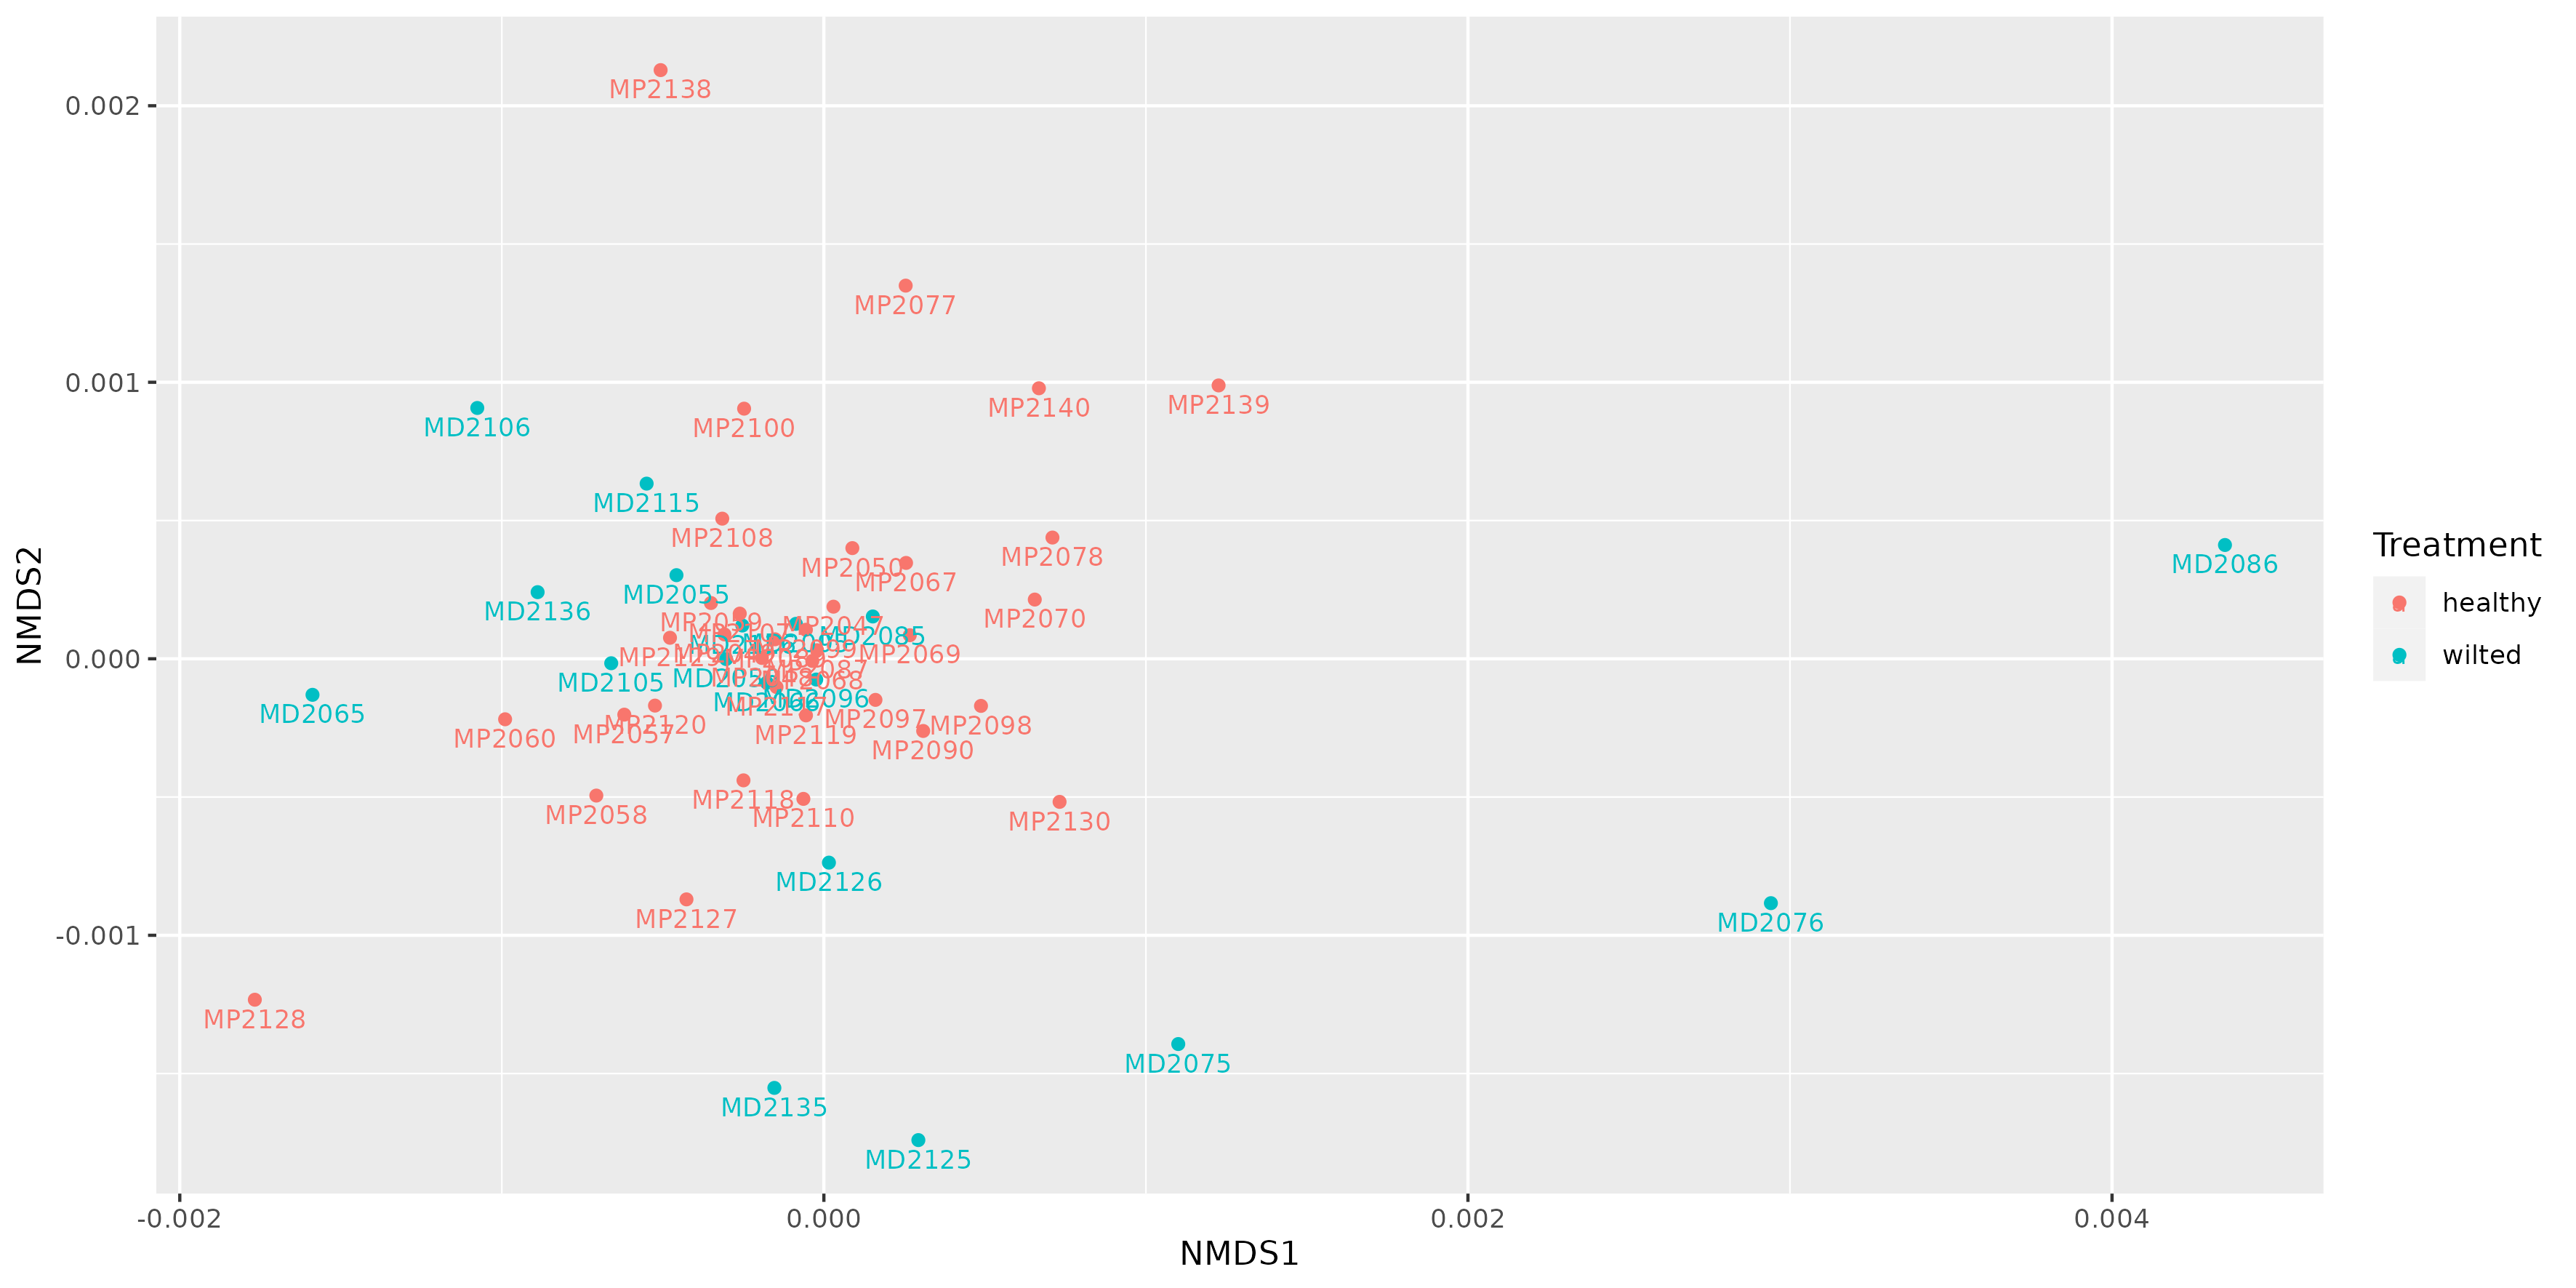
\includegraphics[width=\textwidth]{Img/cap2/DiversidadBetaFresaKraken_fil_euclidean.png}
\caption{Diversidad Beta, distancia Euclidiana, \href{https://github.com/CamilaSilva1995/Tesis_Maestria/blob/main/Analisis_Comparativo/Fresa_Solena/01_Exploracion.Rmd}{(Exploracion.Rmd)}}
\end{figure}

La distancia \textbf{Manhattan} también se emplea en el análisis de datos numéricos y se basa en la diferencia de las abundancias o proporciones de diferentes especies en distintas muestras. En este caso, la distancia de Manhattan entre dos muestras se define como la suma de las diferencias absolutas entre las proporciones de cada especie en ambas muestras.

La fórmula de la distancia de Manhattan entre dos muestras $A$ y $B$ se calcula como:
$$d_{Manhattan}(A, B) = \sum{|A_i - B_i|}$$
Donde $A_i$ y $B_i$ son las abundancias o proporciones de la especie $i$ en las muestras $A$ y $B$, respectivamente. \\

Al igual que la distancia Euclidiana, la distancia de Manhattan es simétrica y satisface la desigualdad del triángulo. Esta métrica es adecuada para comparar muestras en términos de las diferencias absolutas en las abundancias de las especies.\\

\begin{figure}[!]
\centering
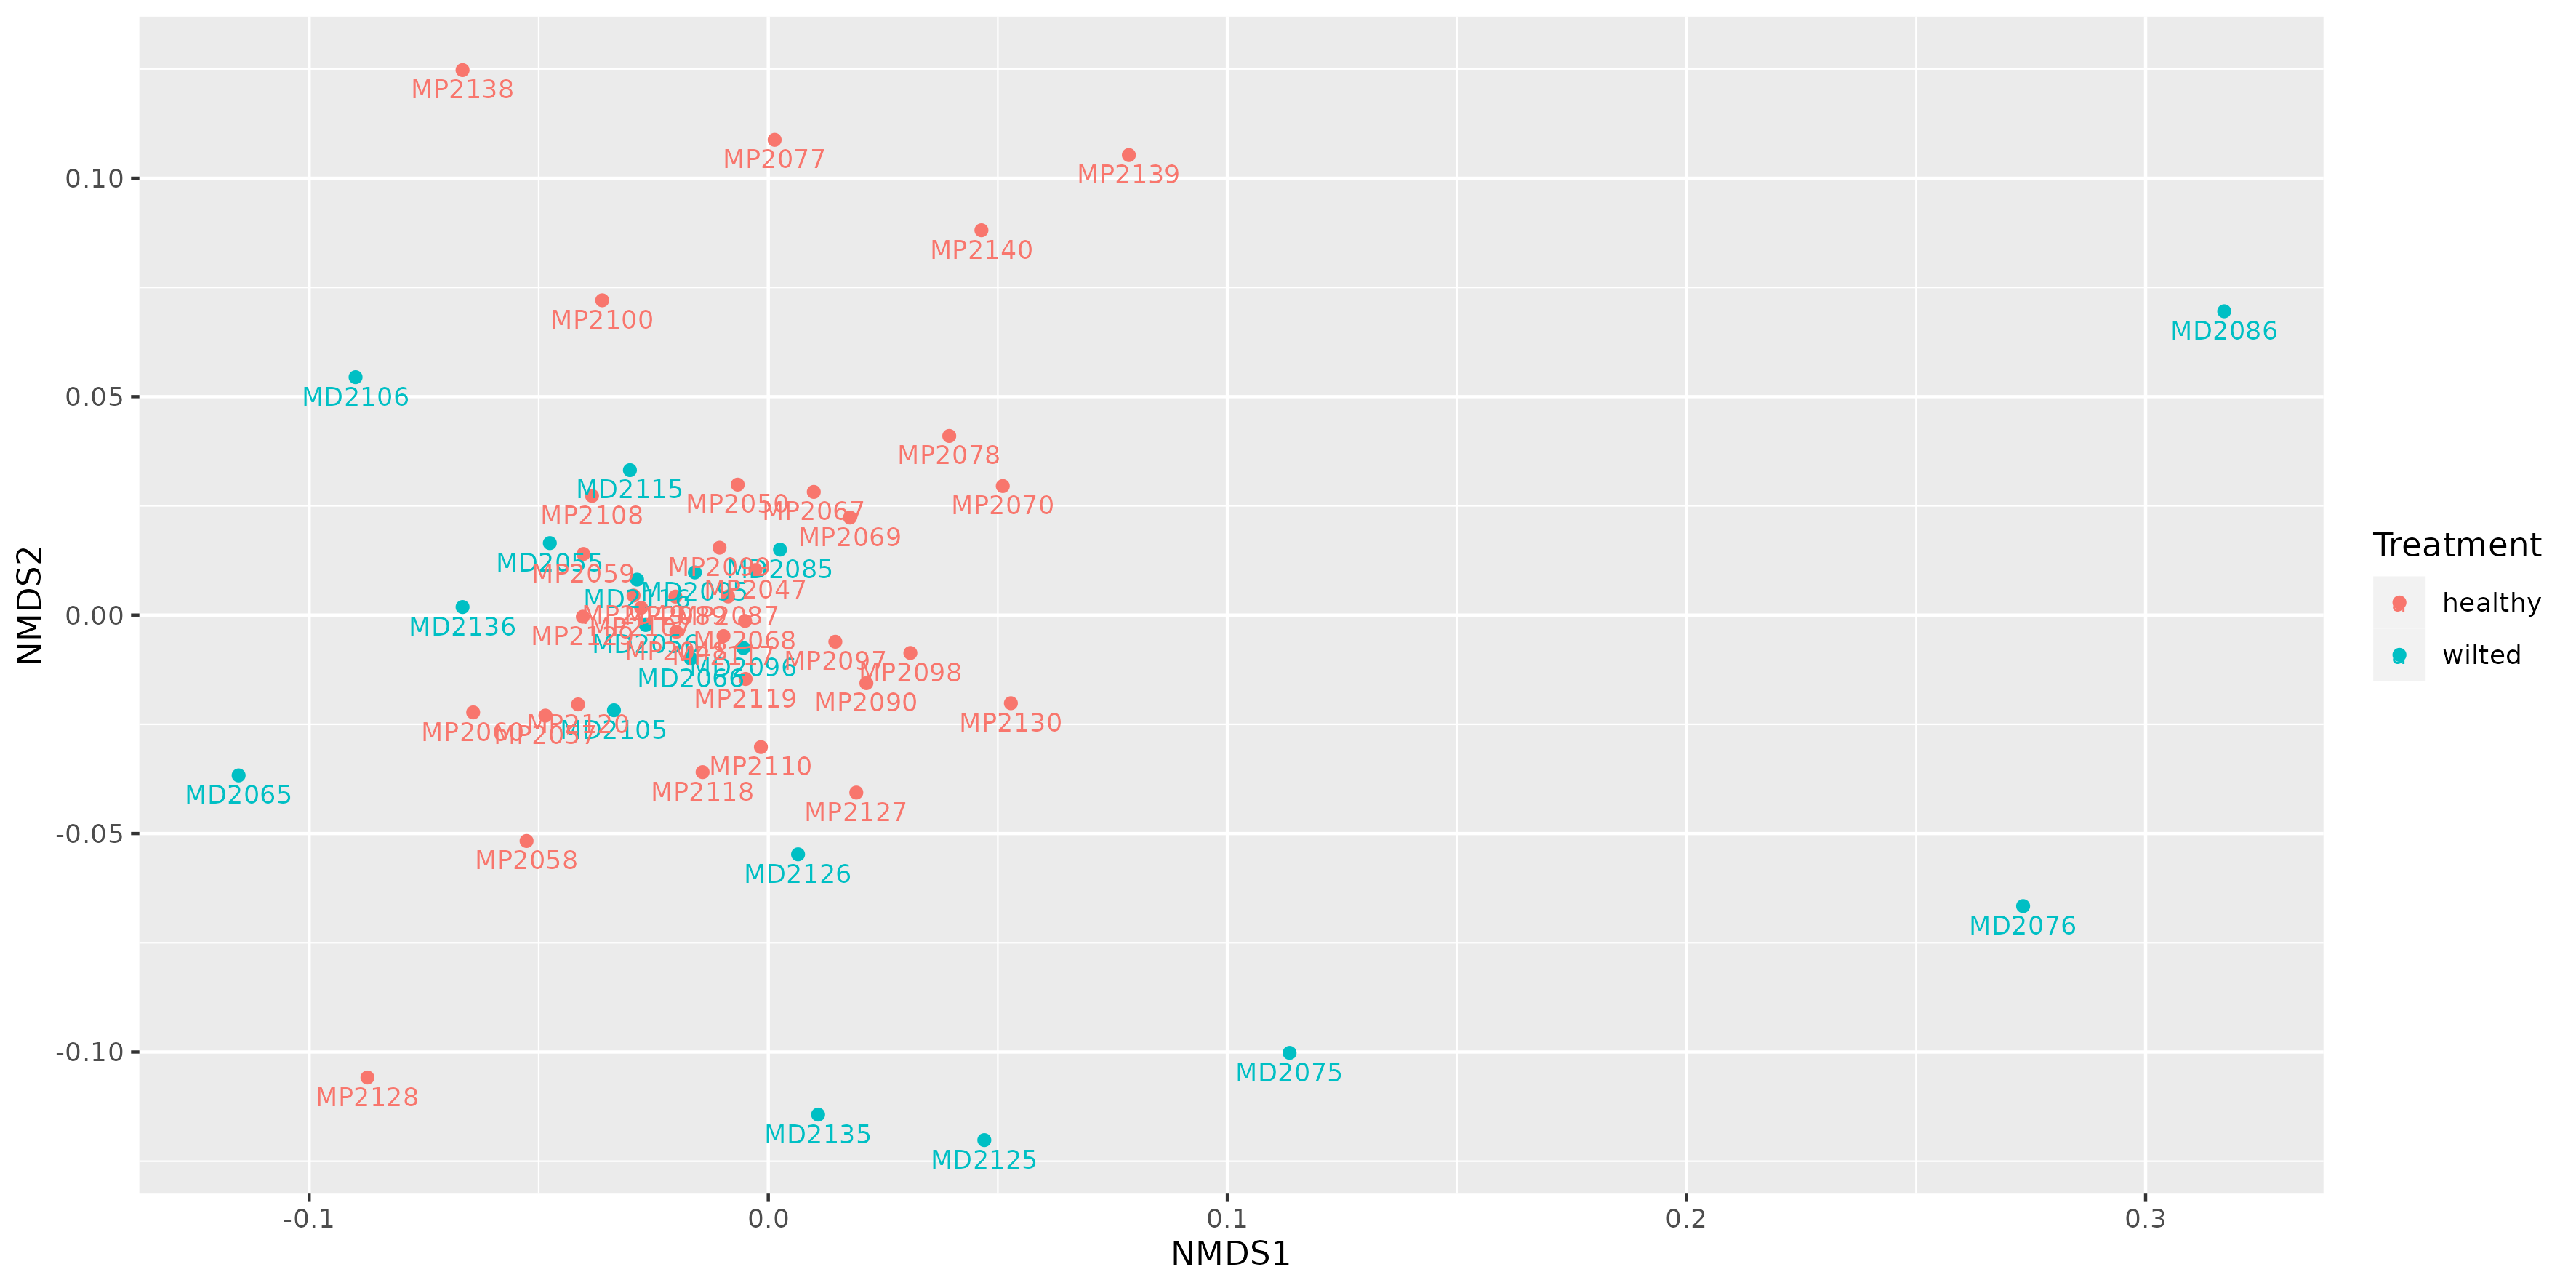
\includegraphics[width=\textwidth]{Img/cap2/DiversidadBetaFresaKraken_fil_manhattan.png}
\caption{Diversidad Beta, distancia Manhattan,  \href{https://github.com/CamilaSilva1995/Tesis_Maestria/blob/main/Analisis_Comparativo/Fresa_Solena/01_Exploracion.Rmd}{(Exploracion.Rmd)}}
\end{figure}

La \textbf{Divergencia de Jensen-Shannon (JSD)} se utiliza para comparar la similitud entre dos distribuciones de probabilidad. En el contexto del análisis de datos de diversidad, estas distribuciones de probabilidad pueden representar la proporción de diferentes especies en distintas muestras. La distancia de JSD entre dos distribuciones de probabilidad se calcula como la raíz cuadrada de la divergencia de Kullback-Leibler entre las dos distribuciones, dividida por dos. 

La fórmula de la distancia de JSD entre dos distribuciones de probabilidad $P$ y $Q$ es la siguiente:
$$d_{JSD}(P, Q) = \frac{\sqrt{(D_{KL}(P, M) + D_{KL}(Q, M))}}{2}$$
Donde $D_{KL}(P, M)$ y $D_{KL}(Q, M)$ son las divergencias de Kullback-Leibler entre las distribuciones $P$ y $Q$ y la media $M$ de ambas distribuciones, respectivamente. \\

Al igual que las distancias anteriores, la distancia de JSD es simétrica y satisface la desigualdad del triángulo. Esta métrica es especialmente útil cuando se quiere evaluar la similitud entre las proporciones de especies en diferentes muestras.\\

\begin{figure}[!]
\centering
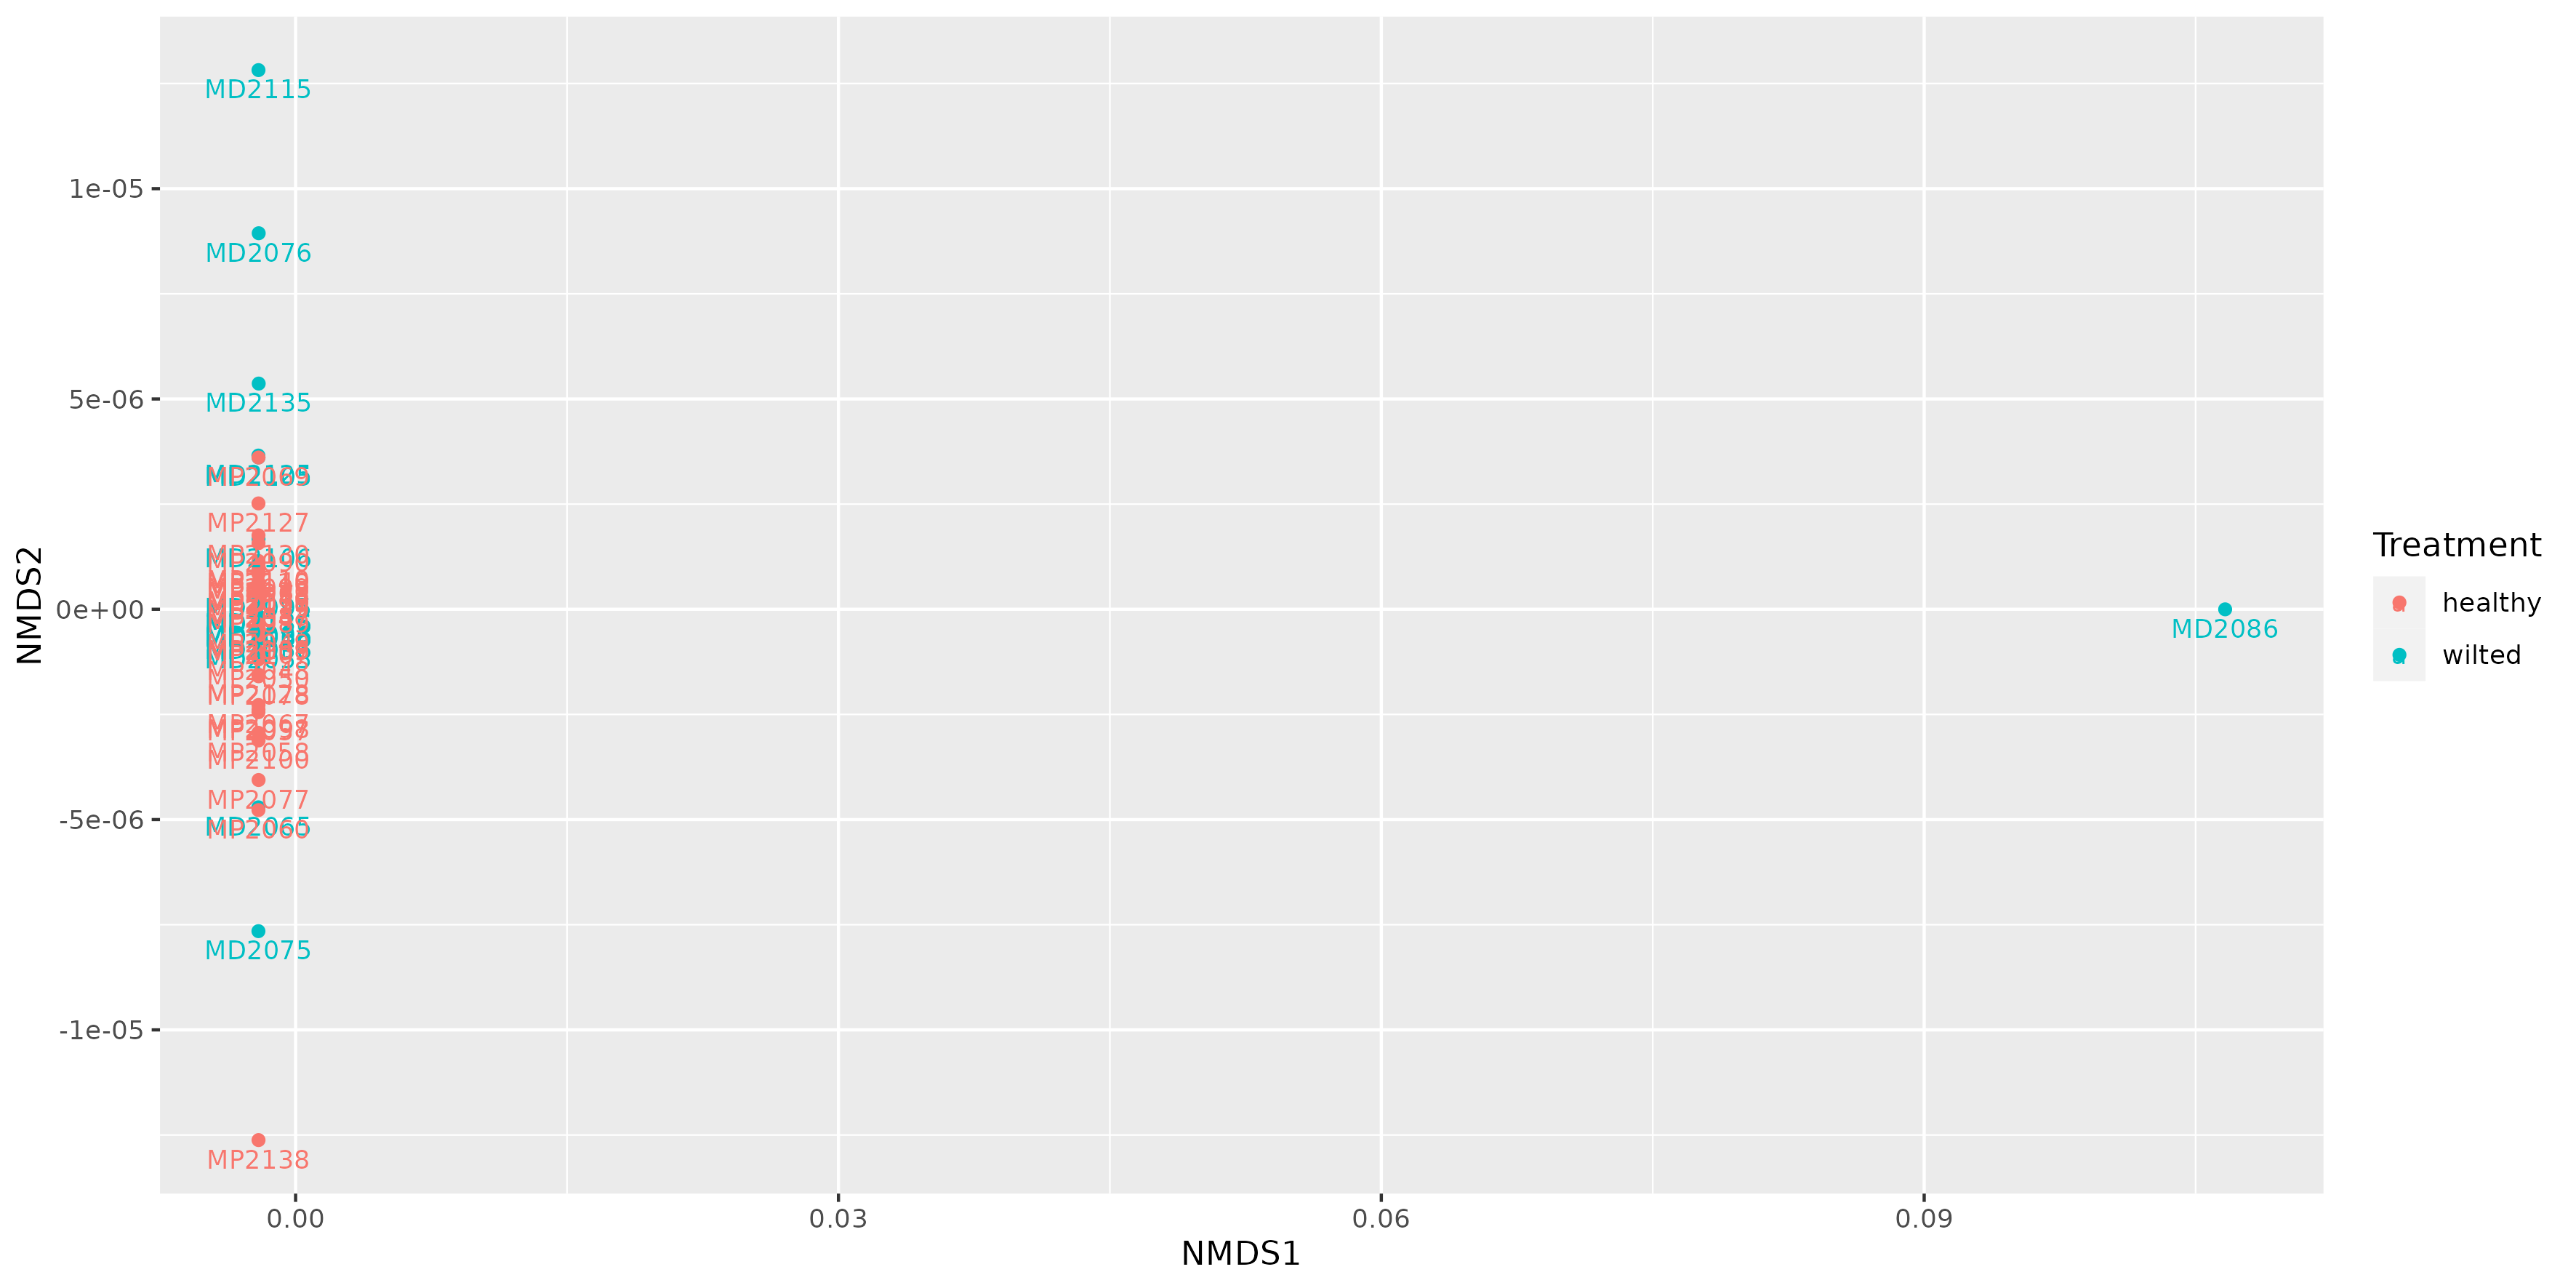
\includegraphics[width=\textwidth]{Img/cap2/DiversidadBetaFresaKraken_fil_jsd.png}
\caption{Diversidad Beta, divergencia de Jensen-Shannon,  \href{https://github.com/CamilaSilva1995/Tesis_Maestria/blob/main/Analisis_Comparativo/Fresa_Solena/01_Exploracion.Rmd}{(Exploracion.Rmd)}}
\end{figure}

La metrica de \textbf{UniFrac} es un índice de disimilitud que se basa en la filogenia de las especies presentes en diferentes sitios. Su objetivo es comparar la similitud entre dos sitios en términos de la diversidad filogenética de las especies, teniendo en cuenta la contribución relativa de cada rama en el árbol filogenético. Esta métrica resulta valiosa para evaluar la similitud en la evolución de las especies en diferentes comunidades o para comparar la estructura filogenética de distintas comunidades.\\

La fórmula del índice de disimilitud de UniFrac es más compleja en comparación con las de Bray-Curtis y Jaccard, ya que se basa en un análisis de la distribución de ramas filogenéticas únicas o compartidas entre los sitios. Este enfoque permite capturar la información sobre las relaciones evolutivas entre las especies, proporcionando una medida más completa de la similitud o disimilitud entre las comunidades estudiadas. \\

Estas métricas ofrecen diferentes perspectivas sobre la similitud o disimilitud entre muestras, permitiendo seleccionar la más apropiada según el contexto del estudio y los objetivos específicos del análisis de diversidad beta.\\

Luego de no ver una clara separacion de los datos, Dado que no se observa una clara separación de los datos, se decide proceder con un análisis en conjuntos más pequeños. Este enfoque puede ayudar a identificar patrones más específicos o diferencias significativas en la composición de especies entre subconjuntos de muestras, lo que contribuirá a una comprensión más detallada de la diversidad microbiana en el contexto particular del estudio.\\

\section{Exploración a distintos niveles taxonómicos}
Podemos visualizar las barras de abundancia absolutas y relativas de nuestros datos representando las muestras en el eje x y las abundancias en el eje y, diferenciando entre muestras sanas y enfermas.\\
\begin{figure}[h]
\centering
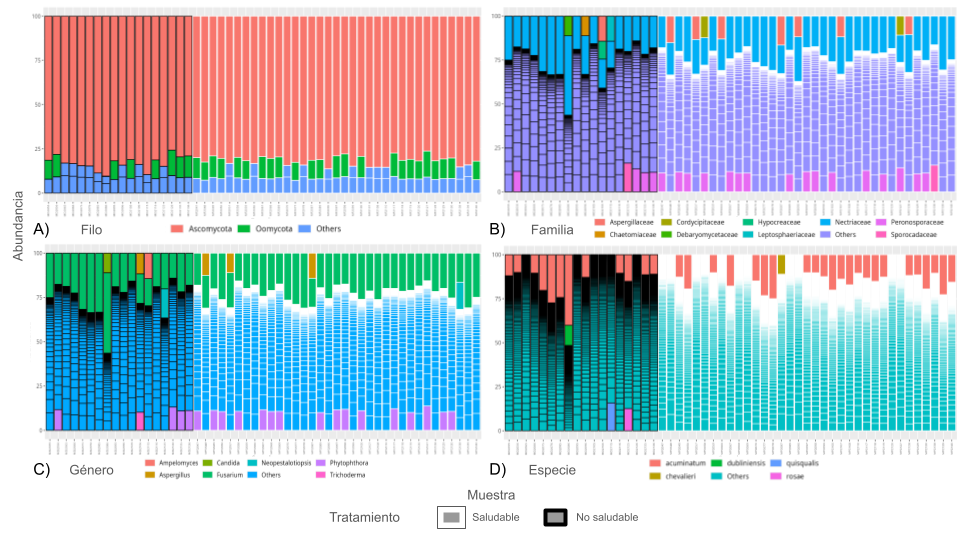
\includegraphics[width=\textwidth]{Img/cap2/Barras_Eukarya10.png}
\caption{A) Barras de abundancias absolutas y B) Relativas}
\end{figure}
Debido a la gran cantidad de datos, resulta difícil discernir diferencias entre las muestras. Por lo tanto, se han creado subconjuntos dividiendo por reino y estableciendo subdivisiones en diferentes niveles taxonómicos.\\

A nivel de filo, ya podemos apreciar una mayor diversidad en nuestras muestras, siendo la mayoría de los filos pertenecientes a bacterias.\\
\begin{figure}[h]
\centering
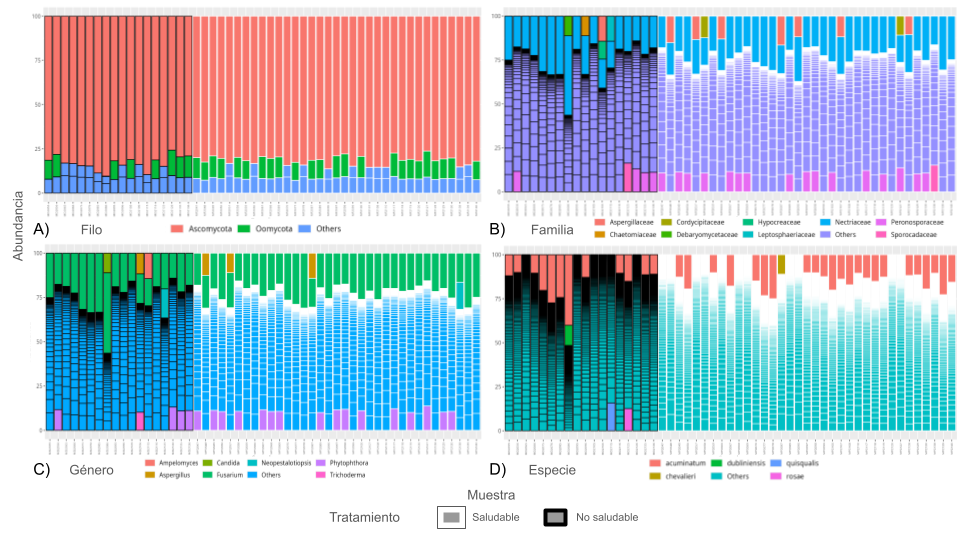
\includegraphics[width=\textwidth]{Img/cap2/Barras_Eukarya10.png}
\caption{A)Barras de abundancias absolutas y B) relativas a nivel de filo}
\end{figure}
Podemos notar algunas diferencias entre los diferentes filos; sin embargo, la gran cantidad de taxones dificulta distinguir adecuadamente el color de cada uno, a menos que tengan una abundancia muy significativa. Dado que nuestro objetivo es diferenciar entre muestras sanas y enfermas, agregaremos una distinción adicional utilizando la variable 'Tratamiento': representaremos las muestras sanas en color blanco y las muestras enfermas en color negro.\\
\begin{figure}[h]
\centering
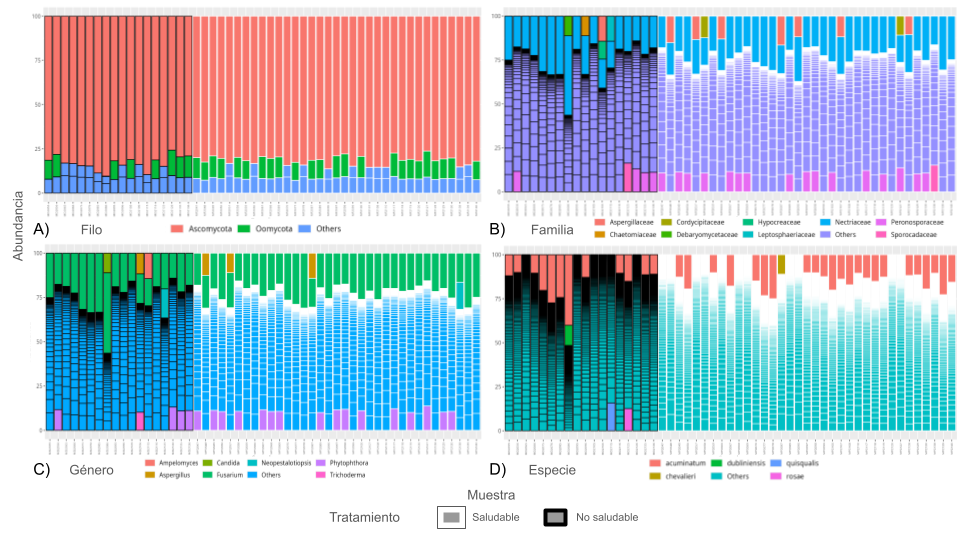
\includegraphics[width=\textwidth]{Img/cap2/Barras_Eukarya10.png}
\caption{Barras de abundancias relativas separando entre sanas y enfermas}
\end{figure}
De igual manera, la cantidad de taxones dificulta la distinción entre las muestras. Por ello, hemos creado subconjuntos más pequeños para facilitar una observación más clara de nuestros datos.\\

En el análisis de diversos grupos taxonómicos, comenzamos examinando gráficos de barras de abundancias como primer paso para seleccionar conjuntos específicos de interés. Al representar las muestras en el eje x y las abundancias en el eje y, obtenemos una visualización clara de las abundancias absolutas y relativas en cada muestra. Este enfoque nos facilita identificar de manera eficiente conjuntos particulares que pueden ser fundamentales para un análisis más detallado y específico.\\

Basándonos en los resultados y medidas anteriores, procedemos a explorar las muestras a diferentes niveles taxonómicos específicos, comenzando con los subconjuntos a nivel de reino, en este caso, Bacteria y Eucariota.\\

Podemos ver cuantos “Eukaryota” tenemos en “Kingdom”.
\begin{lstlisting}[basicstyle=\small] 
sum(fresa_kraken_fil@tax_table@.Data[,"Kingdom"]=="Eukaryota")
## [1] 181
\end{lstlisting}
\begin{lstlisting}[basicstyle=\small] 
sum(fresa_kraken_fil@tax_table@.Data[,"Kingdom"]=="Bacteria")
## [1] 8822
\end{lstlisting}

Al verificar lo observado anteriormente con la agrupación de subconjuntos, confirmamos que hay una mayor cantidad de muestras clasificadas como bacterias en comparación con las clasificadas como eucariotas.\\

A partir de estos dos subconjuntos, llevamos a cabo una agrupación adicional por filo, familia, género y especie. La elección de estos niveles taxonómicos se basa en diferentes propósitos: el filo se selecciona como el siguiente nivel después del reino para proporcionar una visualización panorámica de los datos; mientras que la familia, el género y la especie se seleccionan para obtener una visualización más detallada y poder identificar diferencias significativas entre los grupos de datos.\\

EXPLICAR COMO Y  POR QUE SACAR EL 10 POR CIENTO\\

\begin{figure}[h]
\centering
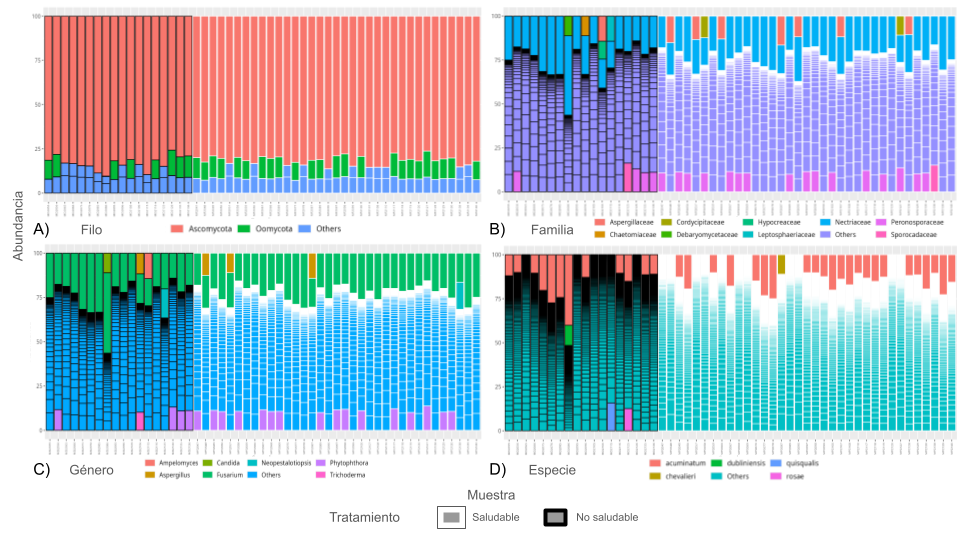
\includegraphics[width=\textwidth]{Img/cap2/Barras_Eukarya10.png}
\caption{Barras de abundancia para eucariota a nivel A) Filo, B) Familia, C) Genero, D) Especie,  \href{https://github.com/CamilaSilva1995/Tesis_Maestria/blob/main/Analisis_Comparativo/Fresa_Solena/20230227_Funciones&Graficas.R}{(FuncionesGraficas.R)}}
\end{figure}

En esta representación a nivel de filo, podemos destacar la disminución notable de \textit{Oomycota} en las muestras enfermas en comparación con las muestras sanas. Al profundizar a nivel de familia, observamos una disminución específica de \textit{Peronosporaceae} en las muestras enfermas en comparación con las muestras sanas.\\

\begin{figure}[h]
\centering
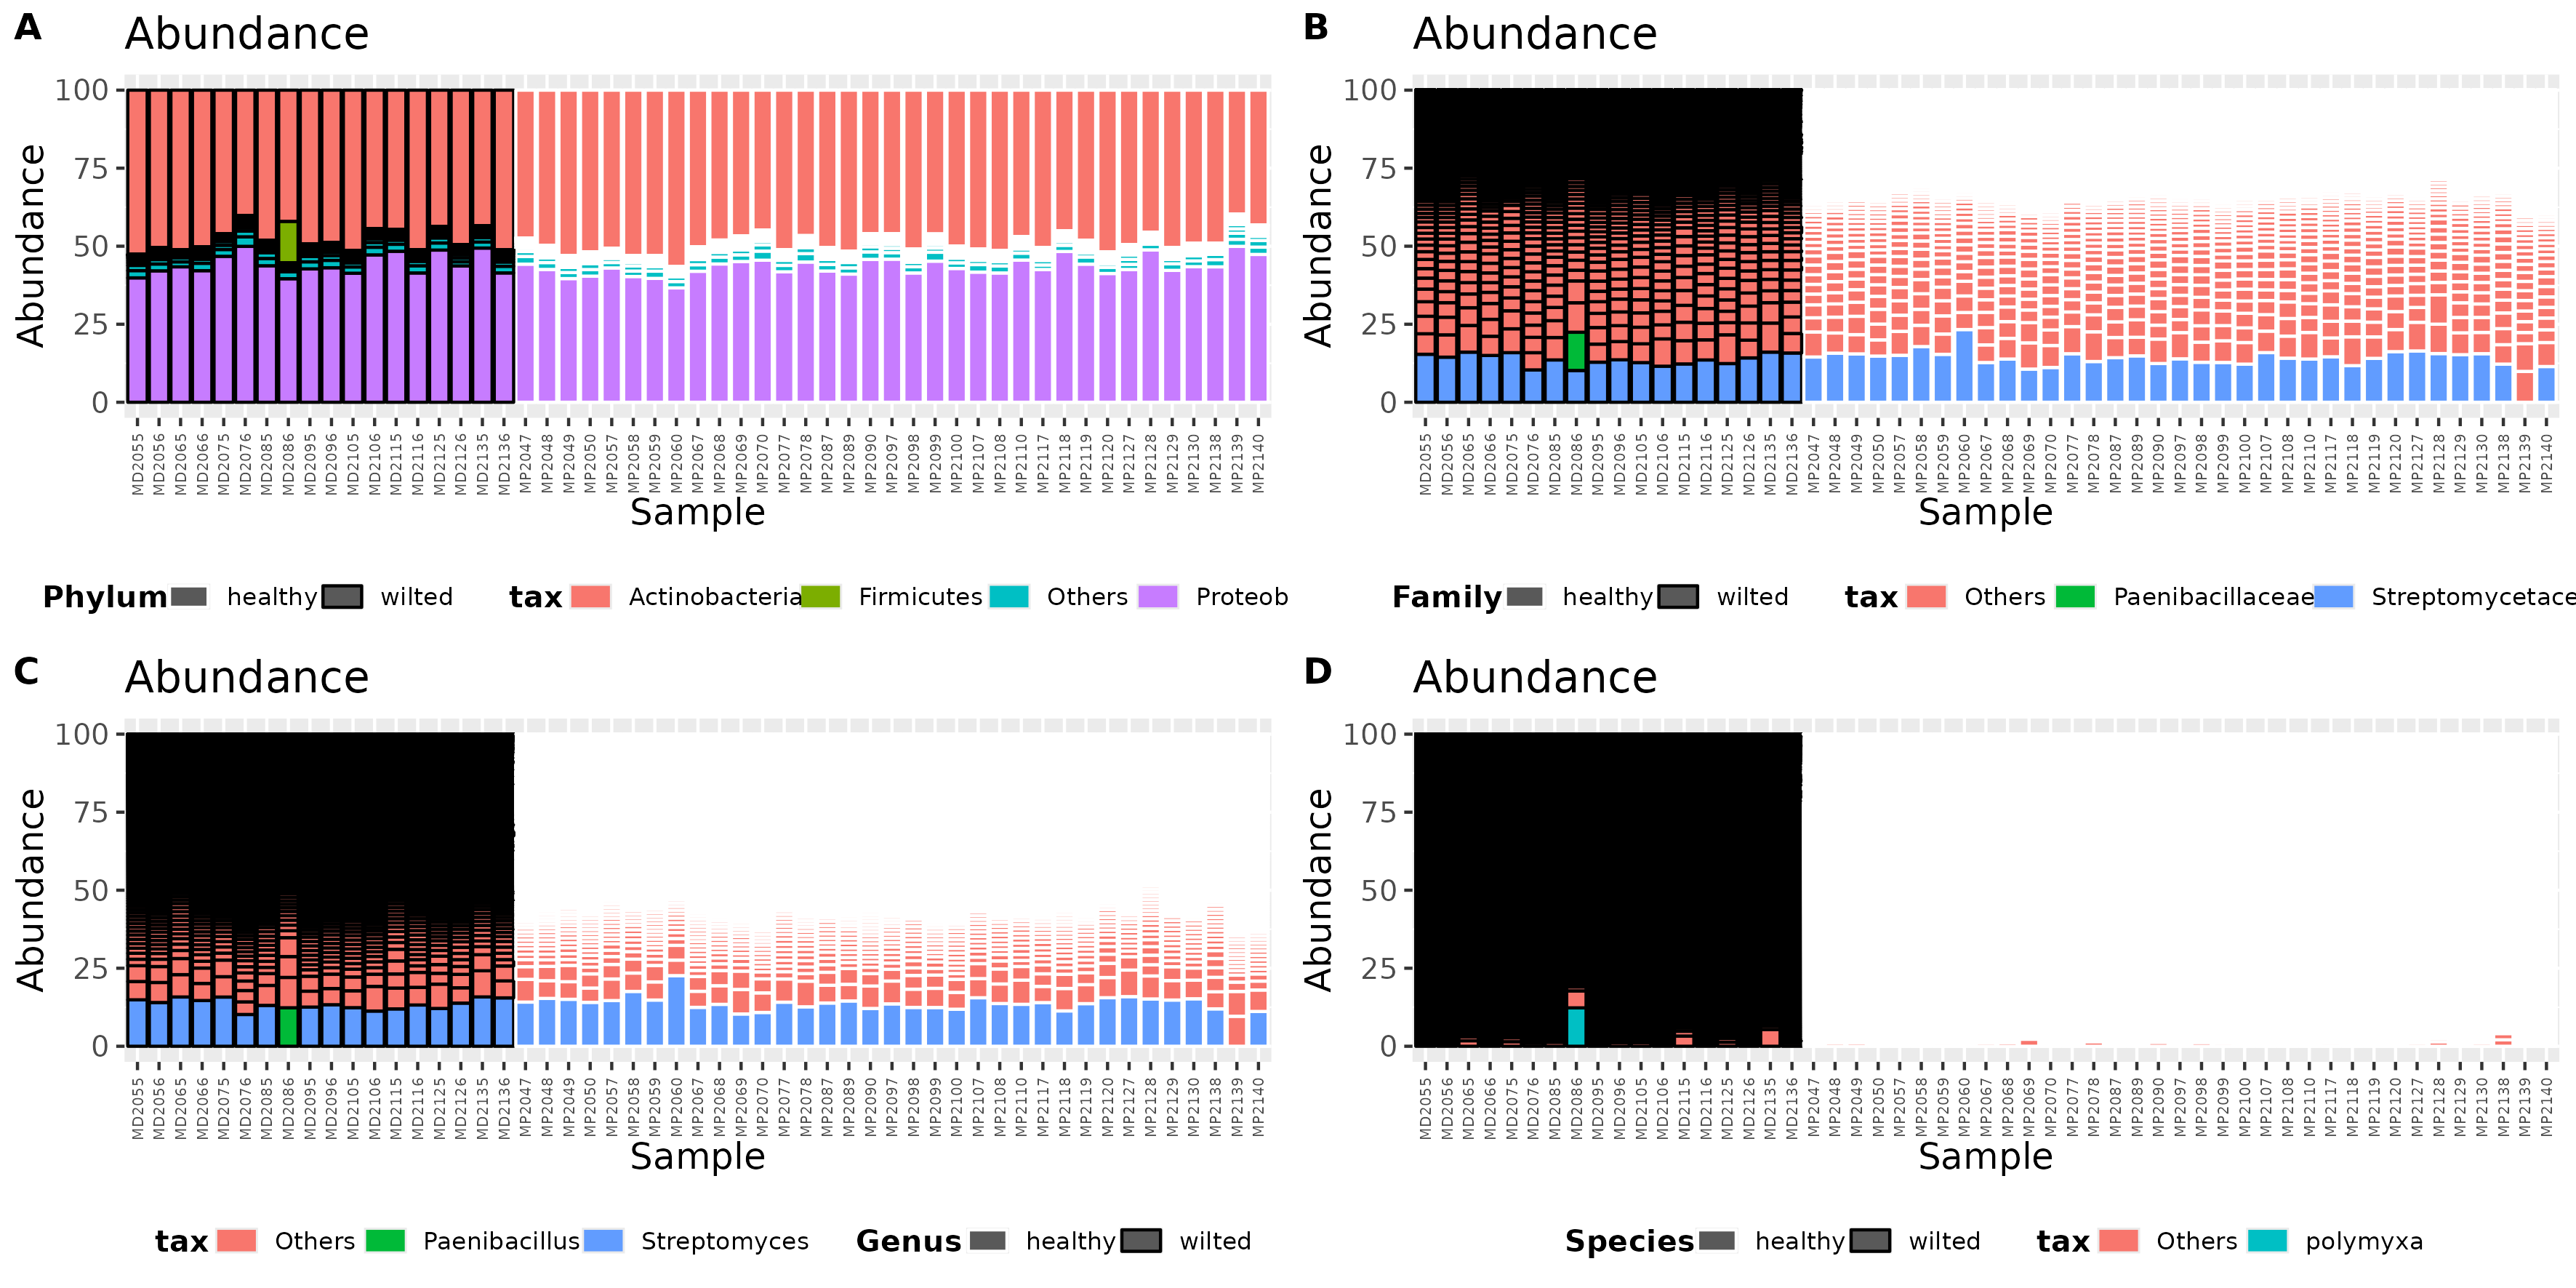
\includegraphics[width=\textwidth]{Img/cap2/Barras_Bacteria10.png}
\caption{Barras de abundancia para bacteria a nivel A) Filo, B) Familia, C) Genero, D) Especie, \href{https://github.com/CamilaSilva1995/Tesis_Maestria/blob/main/Analisis_Comparativo/Fresa_Solena/20230227_Funciones&Graficas.R}{(FuncionesGraficas.R)}}
\end{figure}

\textbf{Diversidad alfa para los niveles taxonomicos}

\begin{figure}[h]
\centering
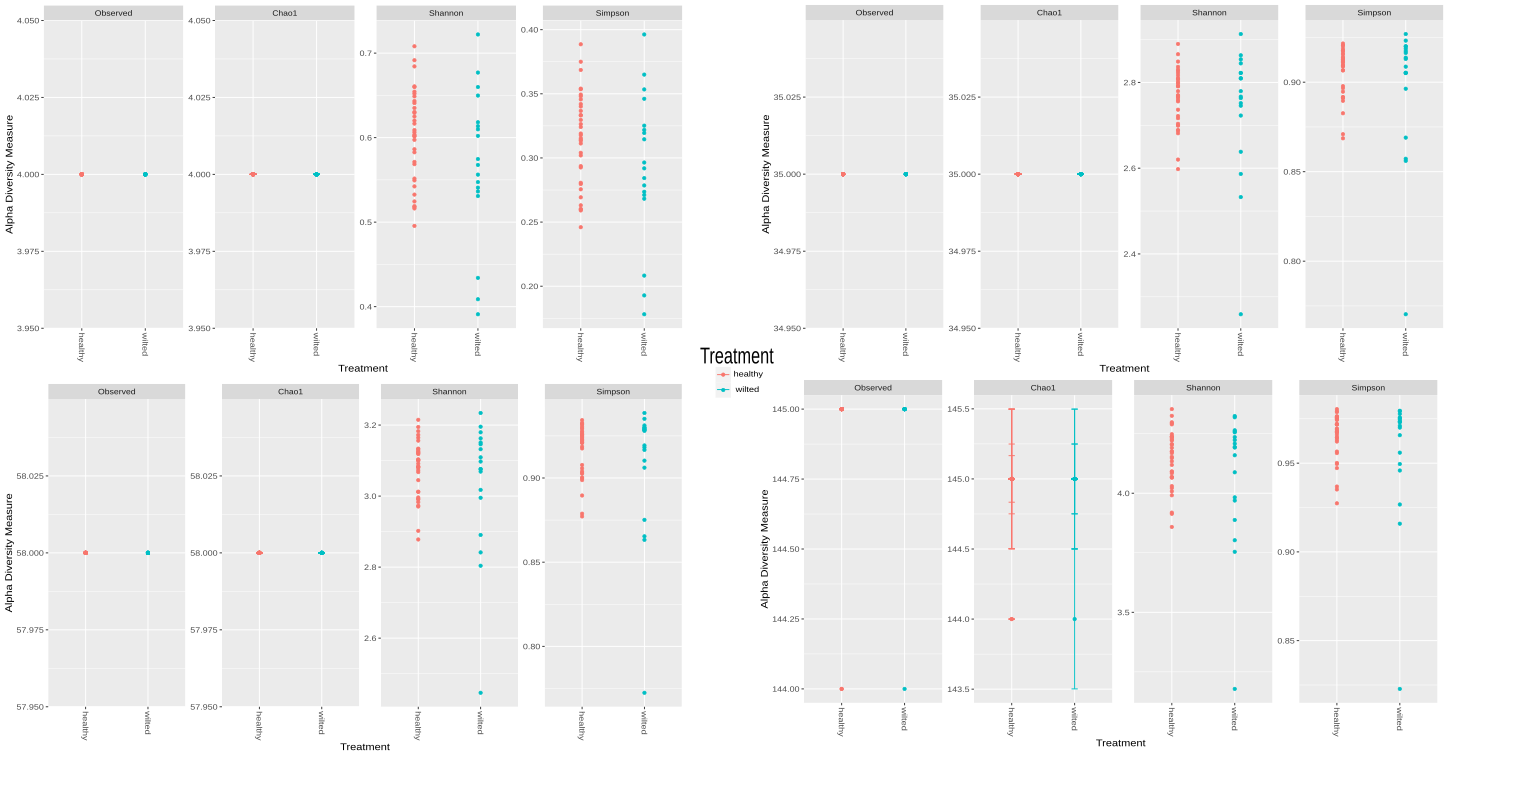
\includegraphics[width=\textwidth]{Img/cap2/Alpha_Eukarya.png}
\caption{Diversidad alpha para eucariota a nivel de A) Filo, B) Familia, C) Genero, D) Especie \href{https://github.com/CamilaSilva1995/Tesis_Maestria/blob/main/Analisis_Comparativo/Fresa_Solena/20230227_Funciones&Graficas.R}{(FuncionesGraficas.R)}}
\end{figure}

En esta imagen, podemos ver que con la diversidad Chao1 a nivel de especie se genera una diferencia considerable de diversidades entre muestras sanas y enfermas, lo cual se detallara mas adelante con una prueba de hipótesis. Tambien ...

\begin{figure}[h]
\centering
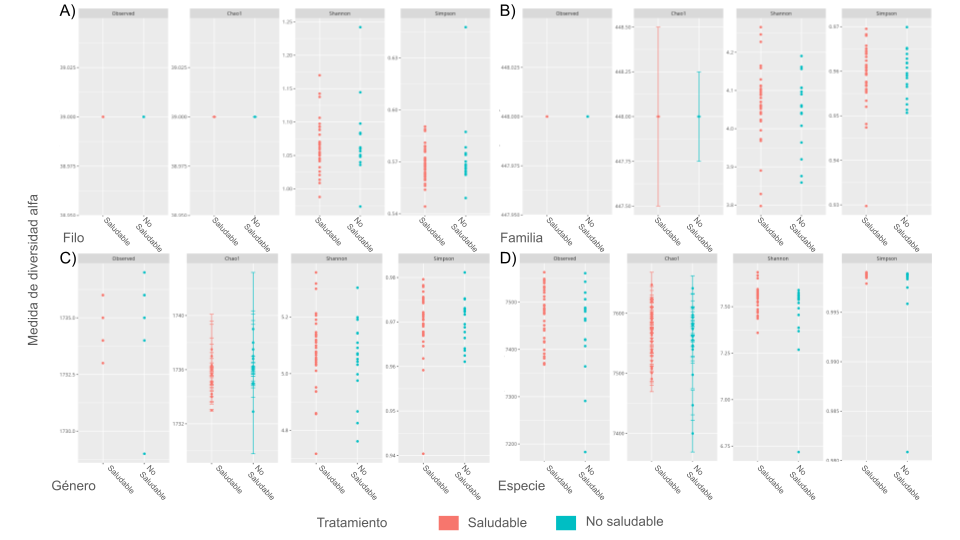
\includegraphics[width=\textwidth]{Img/cap2/Alpha_Bacteria.png}
\caption{Diversidad alpha para bacteria a nivel de A) Filo, B) Familia, C) Genero, D) Especie \href{https://github.com/CamilaSilva1995/Tesis_Maestria/blob/main/Analisis_Comparativo/Fresa_Solena/20230227_Funciones&Graficas.R}{(FuncionesGraficas.R)}}
\end{figure}

En esta imagen, podemos ver que con la diversidad Chao1 a nivel de género se evidencia una diferencia considerable de diversidades entre muestras sanas y enfermas, lo cual se detallara mas adelante con una prueba de hipótesis. Tambien ...

\textbf{Diversidad beta para los niveles taxonomicos}

\begin{figure}[h]
\centering
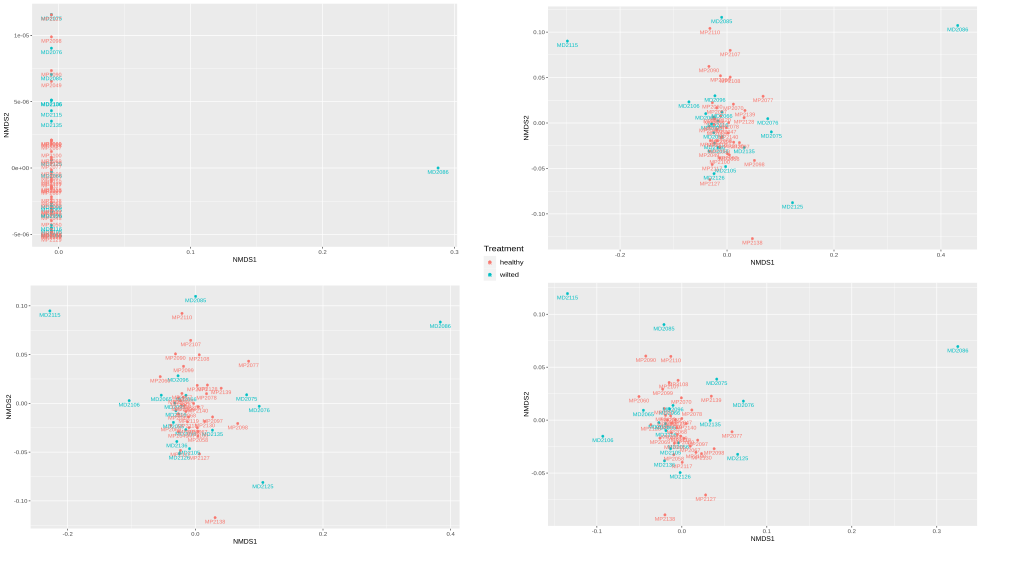
\includegraphics[width=\textwidth]{Img/cap2/Beta_Eukarya.png}
\caption{Diversidad beta para eucariota a nivel de A) Filo, B) Familia, C) Genero, D) Especie \href{https://github.com/CamilaSilva1995/Tesis_Maestria/blob/main/Analisis_Comparativo/Fresa_Solena/20230227_Funciones&Graficas.R}{(FuncionesGraficas.R)}}
\end{figure}

\begin{figure}[h]
\centering
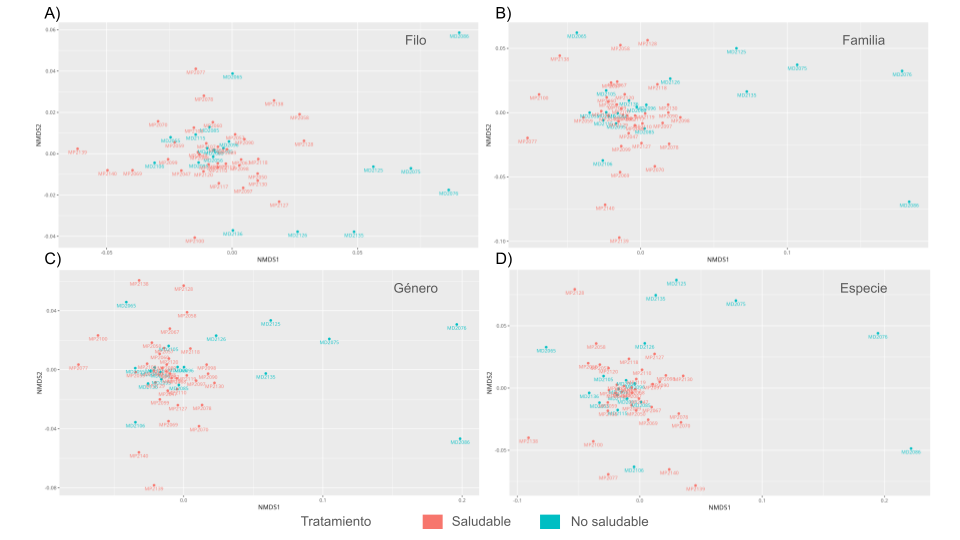
\includegraphics[width=\textwidth]{Img/cap2/Beta_Bacteria.png}
\caption{Diversidad beta para bacteria a nivel de A) Filo, B) Familia, C) Genero, D) Especie \href{https://github.com/CamilaSilva1995/Tesis_Maestria/blob/main/Analisis_Comparativo/Fresa_Solena/20230227_Funciones&Graficas.R}{(FuncionesGraficas.R)}}
\end{figure}


\section{Prueba de Hipótesis}

Procedimiento para evaluar la veracidad de una afirmación científica.
Una prueba de hipótesis es un método estadístico que se utiliza para tomar decisiones sobre una población basándose en una muestra de datos.





%\begin{figure}[!]
%centering
%\includegraphics[width=\textwidth]{Img/cap2/imagen de ejemplo p-valor.png}
%\caption{imagen de ejemplo %p-valor}
%\end{figure}

\textbf{P\_Valor}, el p\-valor se toma como una medida de probabilidad de exito (obtener un resultado especifico), de un estudio estadistico con datos observados.

El calculo de este valor, depende de la prueba estadistica a usar y de las suposiciones hechas sobre la distribución de los datos. En general un valor pequeño del p-valor sugiere que los datos observados son poco probables bajo la hipótesis.

Rice, J. A. (2006). Mathematical Statistics and Data Analysis (3rd ed.)
Wasserman, L. (2004). All of Statistics: A Concise Course in Statistical Inference.

EL p-valor se aplica a la teoría de decision, cuando se tiene dos hipótesis sobre una población.

Hipotesis 
Suposición sobre los datos, la cual puede ser cierta o falsa.

$H_0$ como hipótesis nula y $H_a$ como hipótesis alternativa.
  
Prueba de Hipotesis
Tecnica de inferencia estadística que permite tomar desiciones sobre suposiciones acerca de una población, basada en la observación.

$\alpha$ = Es el nivel de significancia, el cual se fija previamente  

x = Es el valor critico observado. 

Dada que la hipotesis nula sea cierta, el p-valor es la probabilidad de obtener el $\alpha$-crítico o más extremo.



A continuación se hacen las siguientes pruebas de hipotesis que parten de esta base, pero se realizan sobre diferentes medidas de los datos 


		

\subsection{Pruebas con muestras pequeñas para comparar dos medias poblacionales}

Suponemos dos poblaciones independientes con distibuciones normales con 

$$\sigma_{1}^{2} = \sigma_{2}^{2}$$

y queremos probar (tenemos como hipotesis nula)

$$H_{0} : \mu_{1} = \mu _{2}$$

respecto a la hipotesis alternativa

$$H_{a} : \mu_{1} \neq \mu _{2}$$

tomando como estadistico de prueba:

$$ T = \frac{\bar{Y_{1}} - \bar{Y_{2}}}{S_{p}\sqrt{\frac{1}{n_{1}} + \frac{1}{n_{2}}}}$$

donde  

$$ S_{p} = \sqrt{\frac{(n_{1}-1)S_{1}^{2} + (n_{2}-1)S_{2}^{2}}{n_{1} + n_{2} - 2}}$$

\begin{figure}[!]
\centering
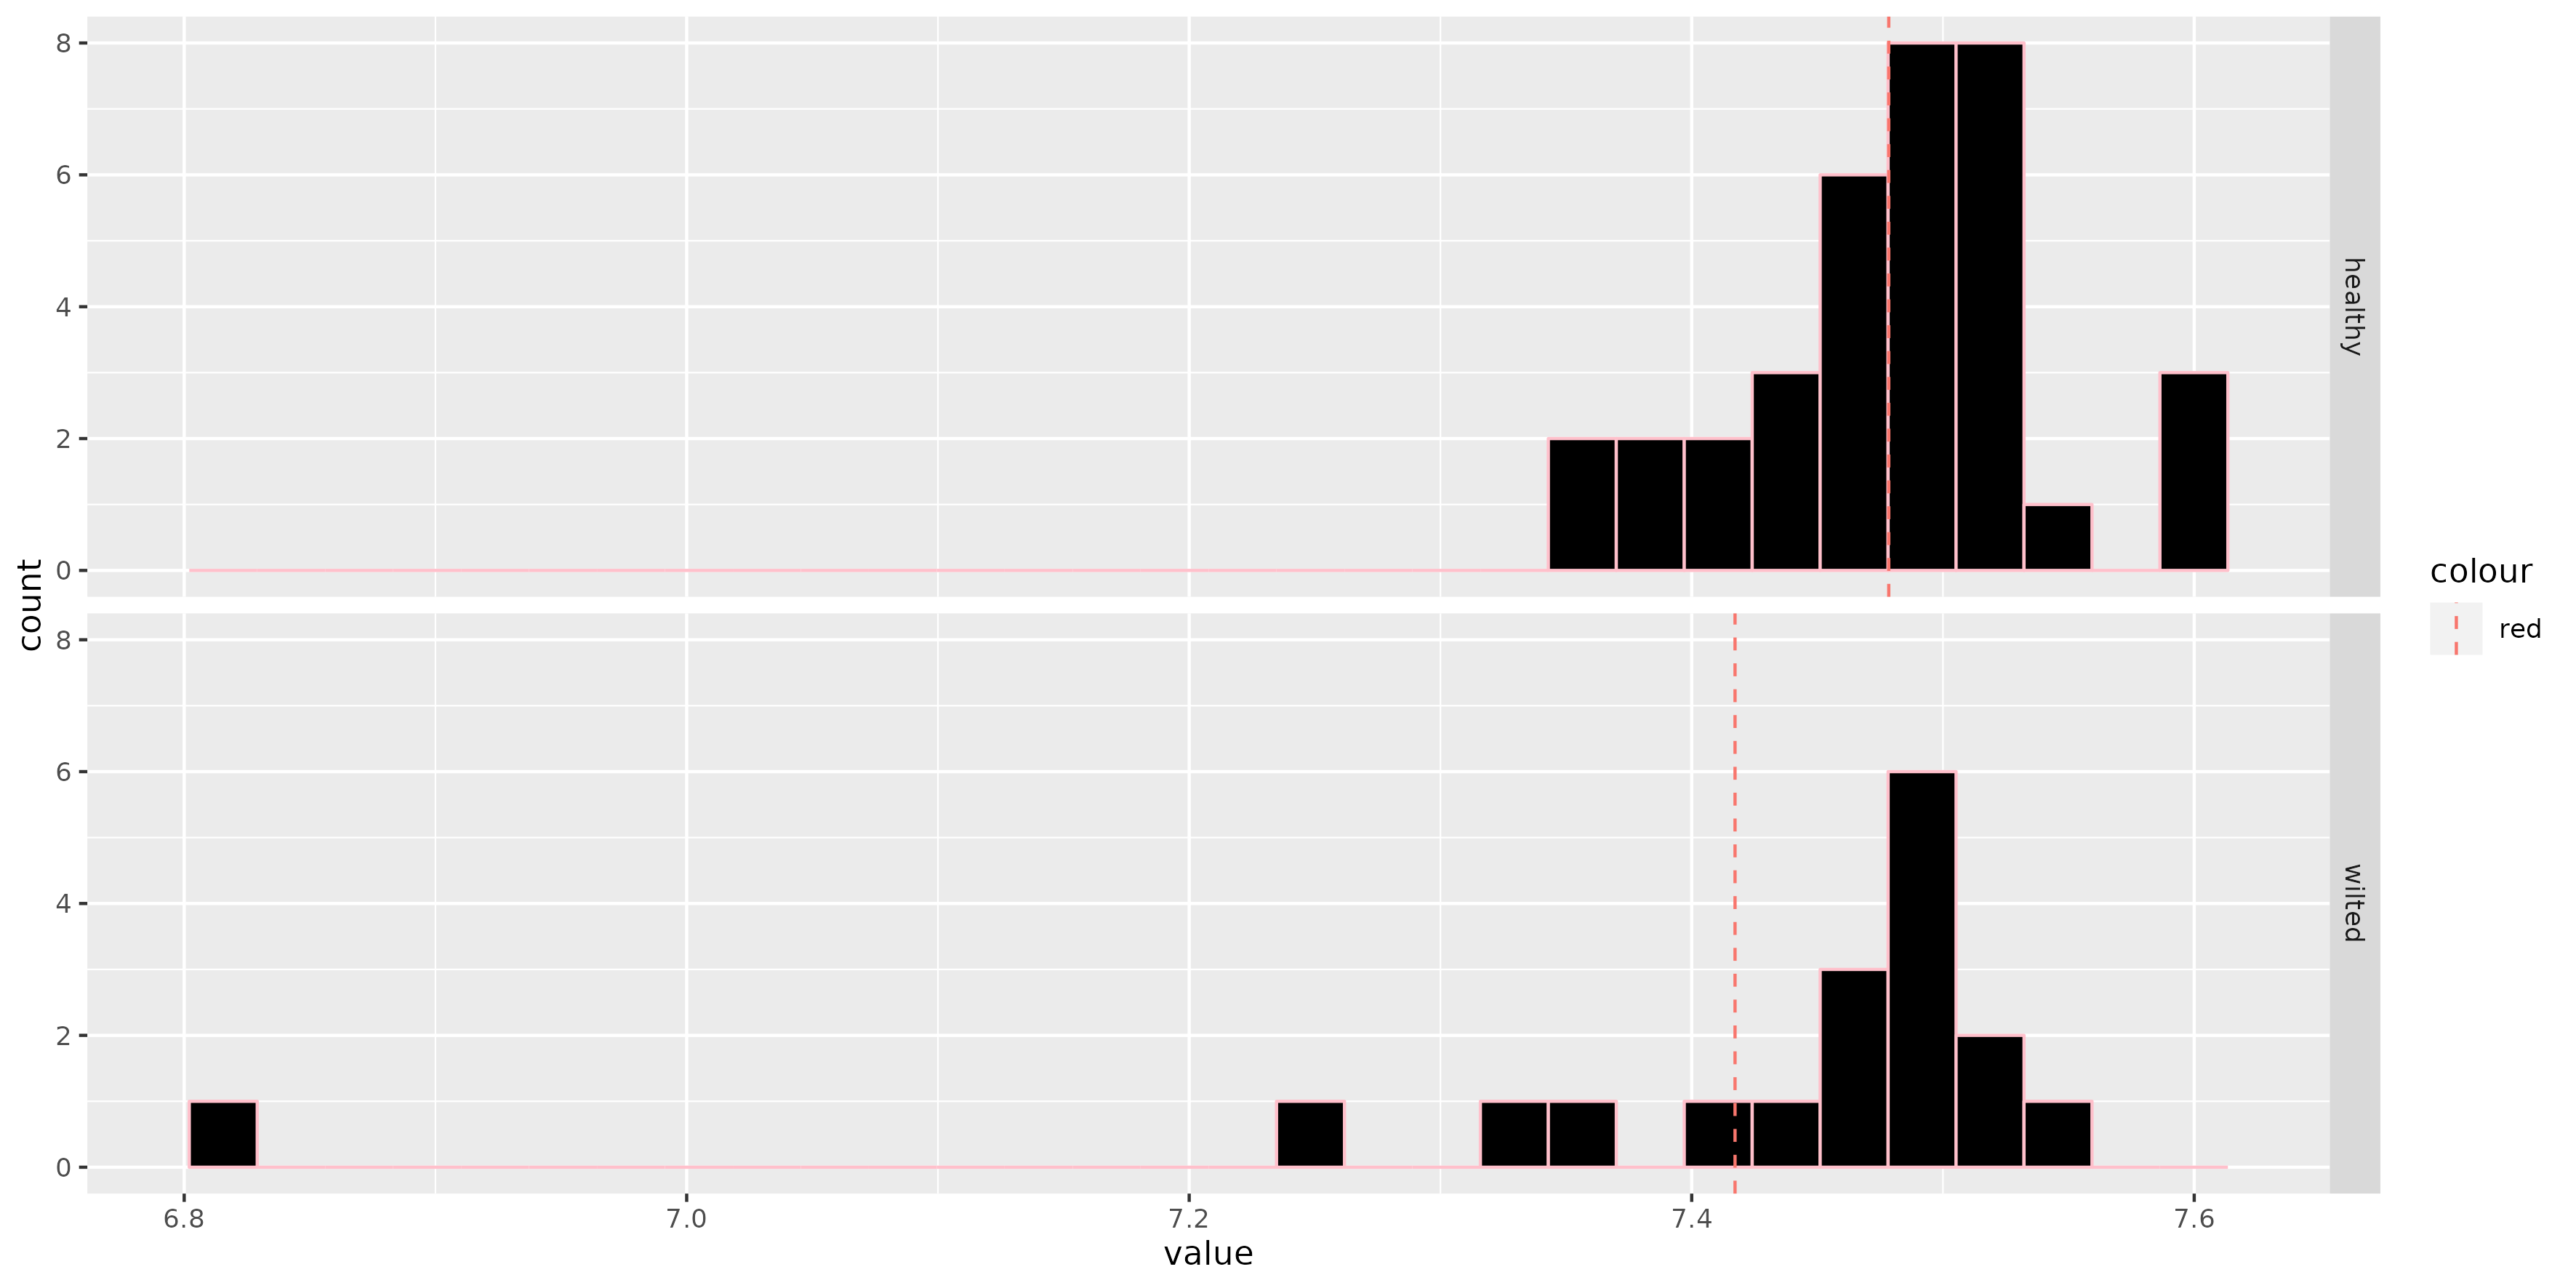
\includegraphics[width=\textwidth]{Img/cap2/medias_Shannon.png}
\caption{}
\end{figure}

\begin{figure}[!]
\centering
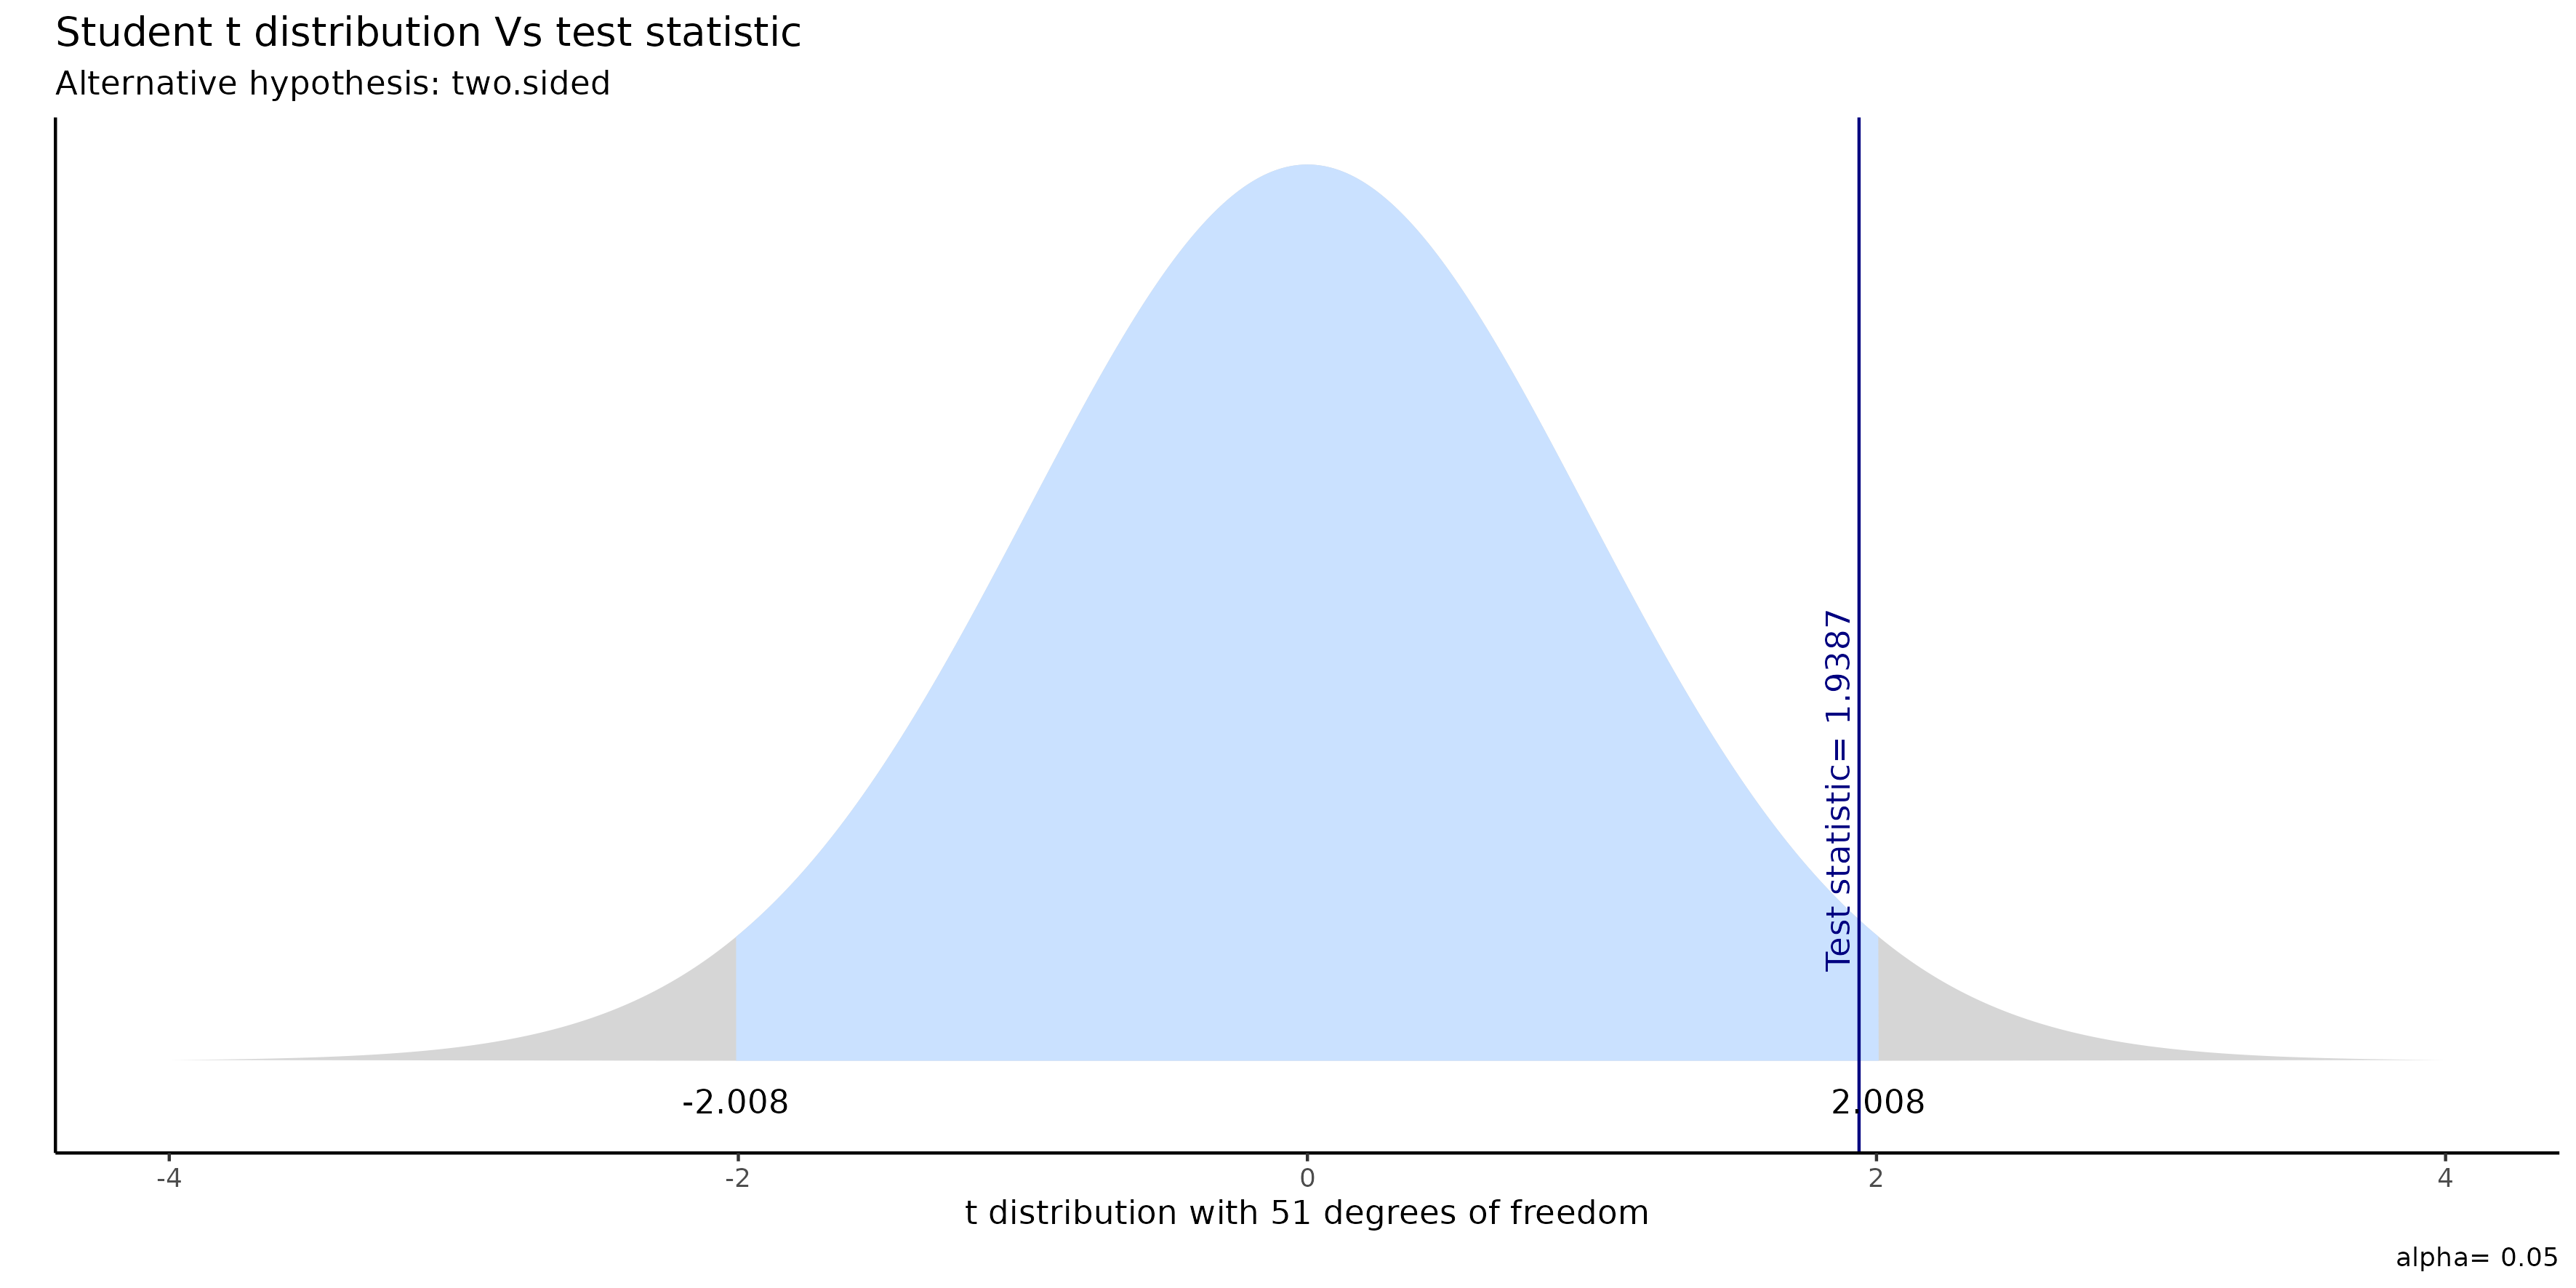
\includegraphics[width=\textwidth]{Img/cap2/pruebat_varianzasiguales_Shannon.png}
\caption{}
\end{figure}

\begin{figure}[!]
\centering
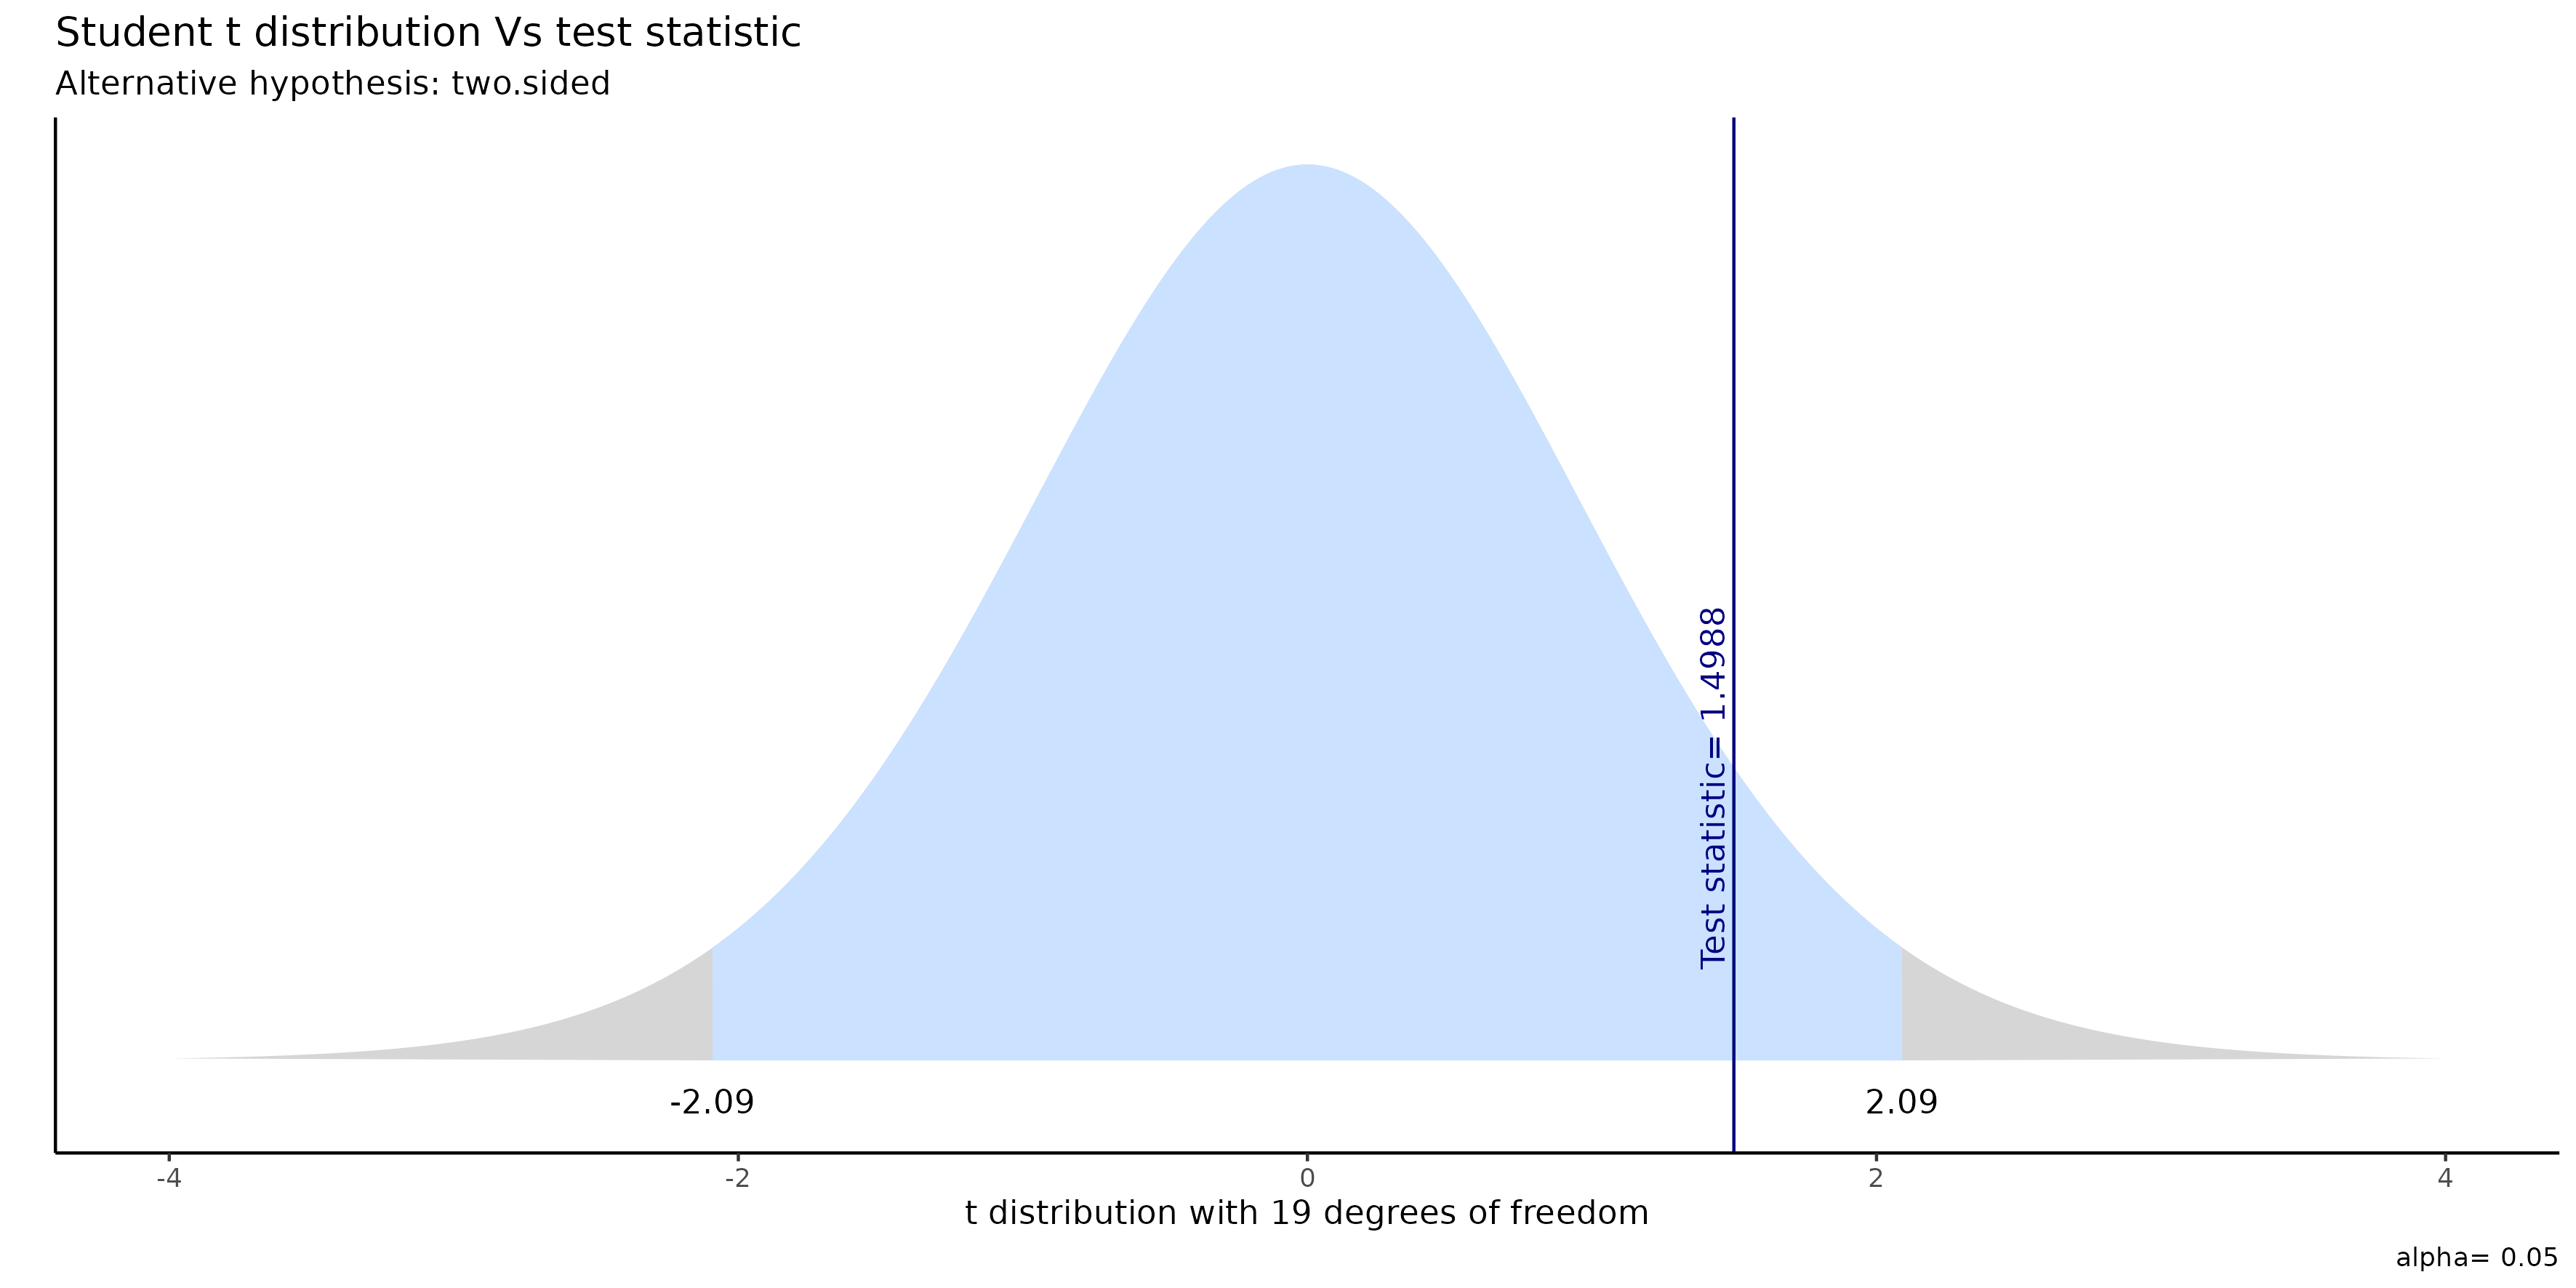
\includegraphics[width=\textwidth]{Img/cap2/pruebat_varianzasdiferentes_Shannon.png}
\caption{}
\end{figure}


\begin{figure}[!]
\centering
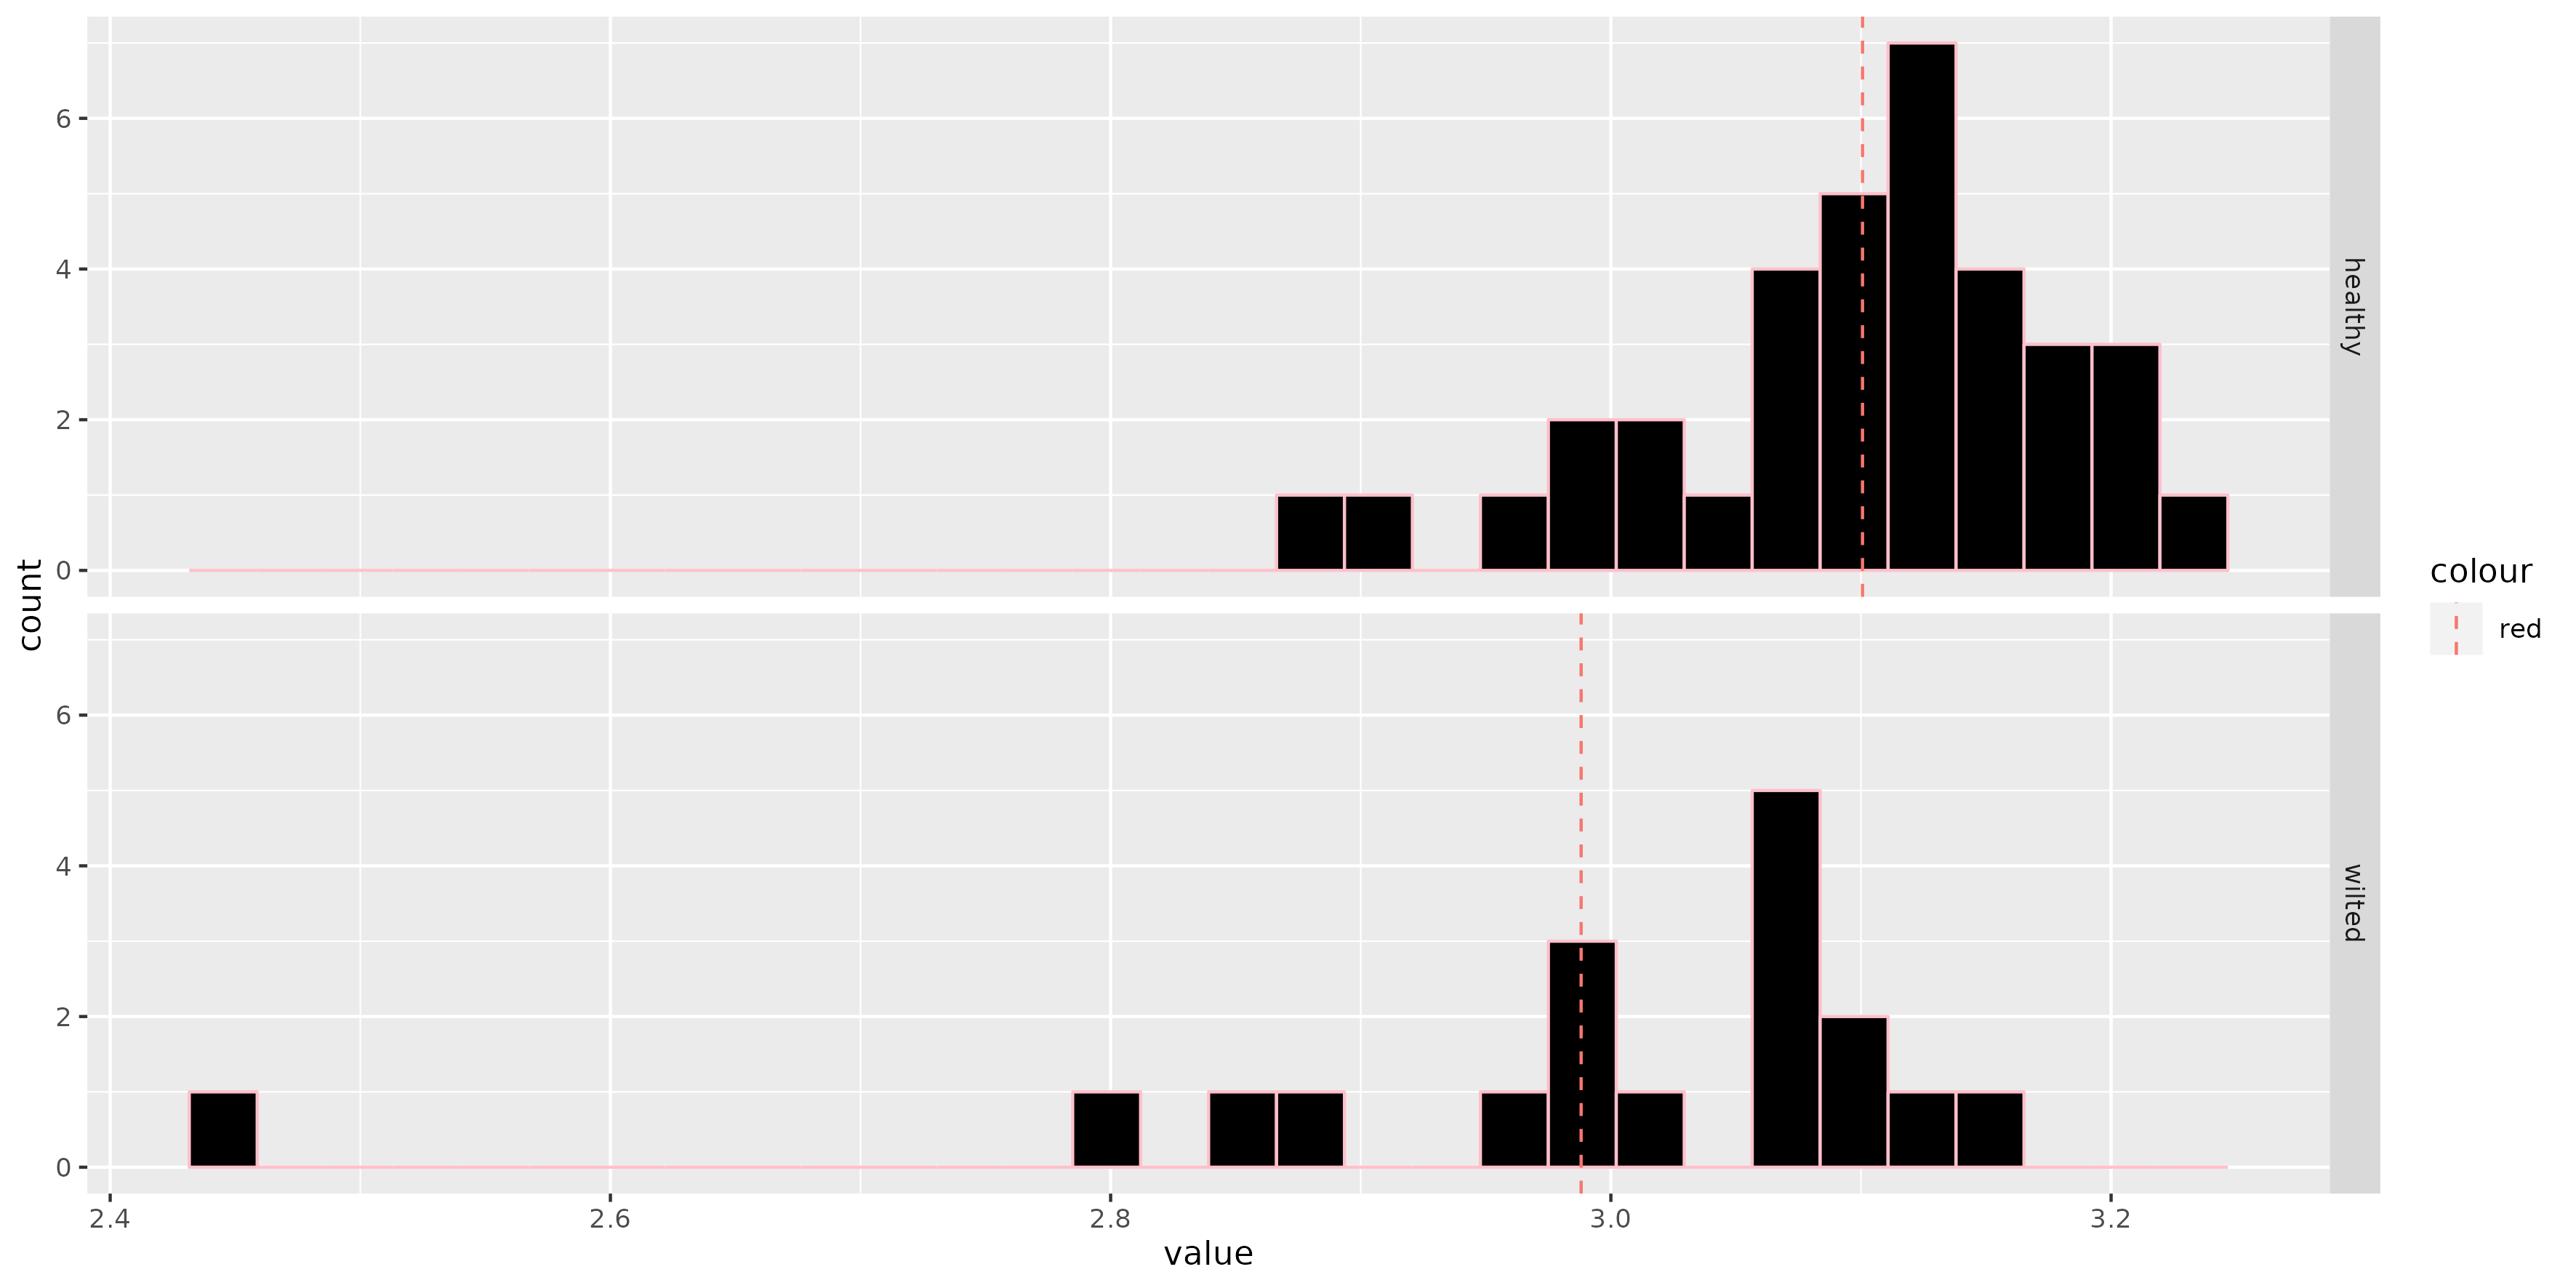
\includegraphics[width=\textwidth]{Img/cap2/mediasFusarium_Shannon.png}
\caption{}
\end{figure}

\begin{figure}[!]
\centering
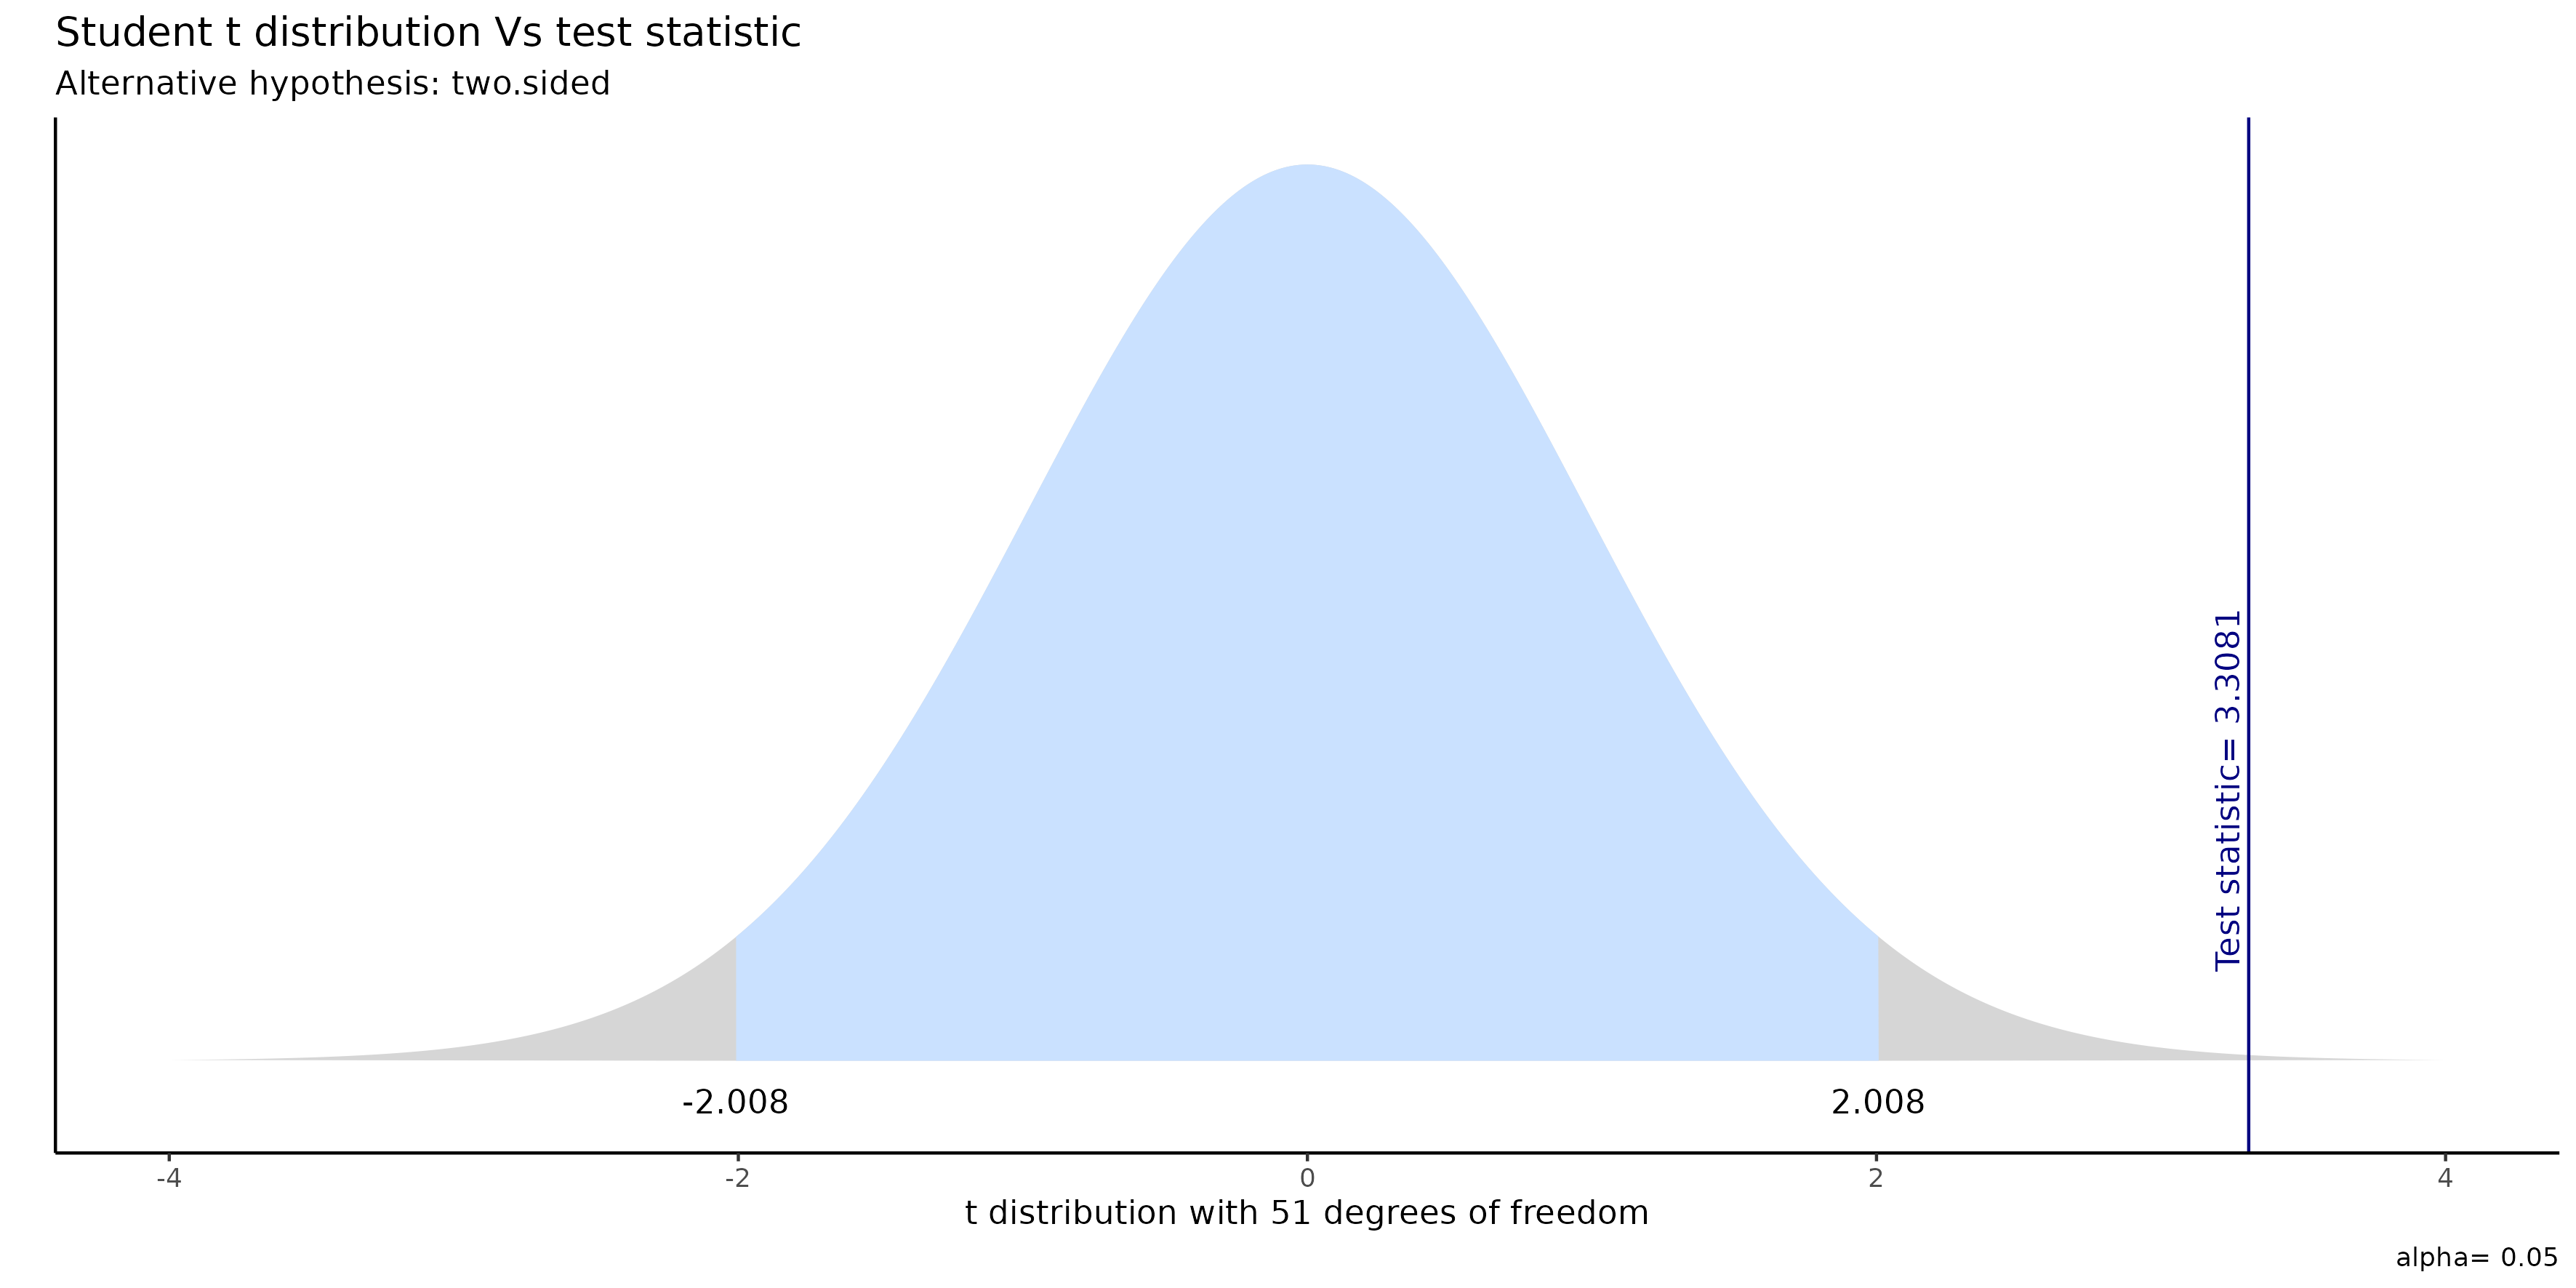
\includegraphics[width=\textwidth]{Img/cap2/pruebat_varianzasigualesFusarium_Shannon.png}
\caption{}
\end{figure}

\begin{figure}[!]
\centering
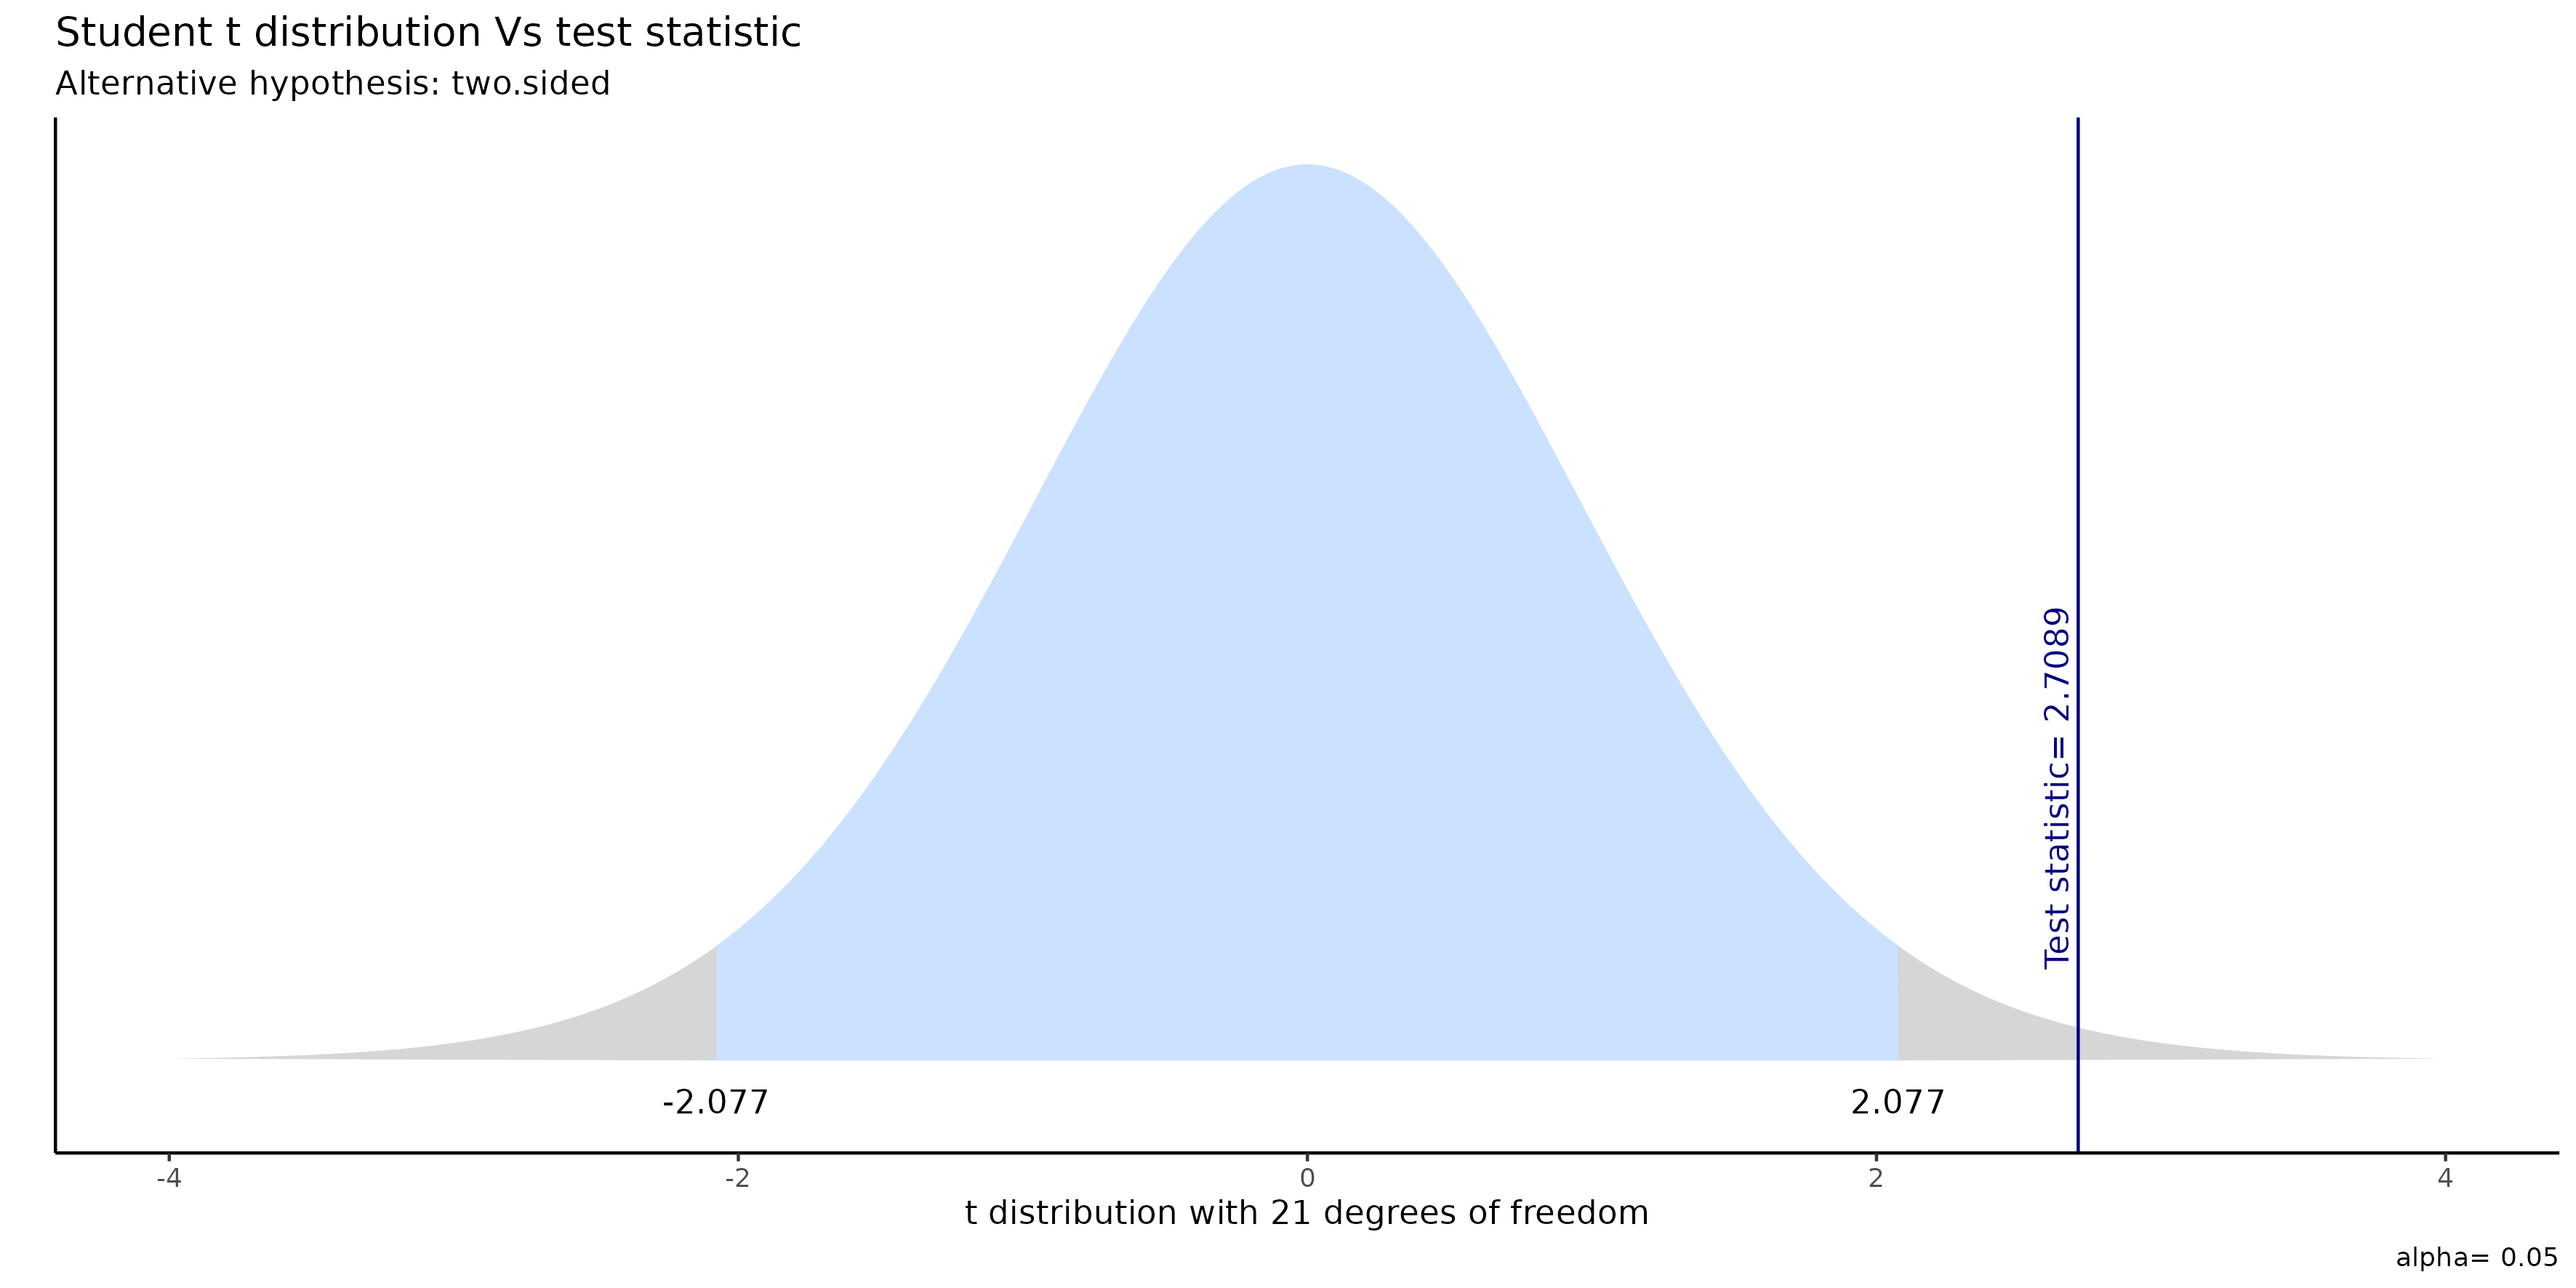
\includegraphics[width=\textwidth]{Img/cap2/pruebat_varianzasdiferentesFusarium_Shannon.png}
\caption{}
\end{figure}

\subsection{Prueba de Hipótesis sobre las varianzas de dos poblaciones pequeñas} 
Pon tu figura y describe tus resultados


Suponemos dos poblaciones independientes con distibuciones normales  

y queremos probar (tenemos como hipotesis nula)WilcoxonWilcoxon

$$H_{0} : \sigma_{1}^{2} = \sigma_{2}^{2}$$

respecto a la hipotesis alternativa

$$H_{a} : \sigma_{1}^{2} \neq \sigma_{2}^{2}$$

tomando como estadistico de prueba:

$$ F = \frac{S_{1}^{2}}{S_{2}^{2}}$$


\begin{figure}[!]
\centering
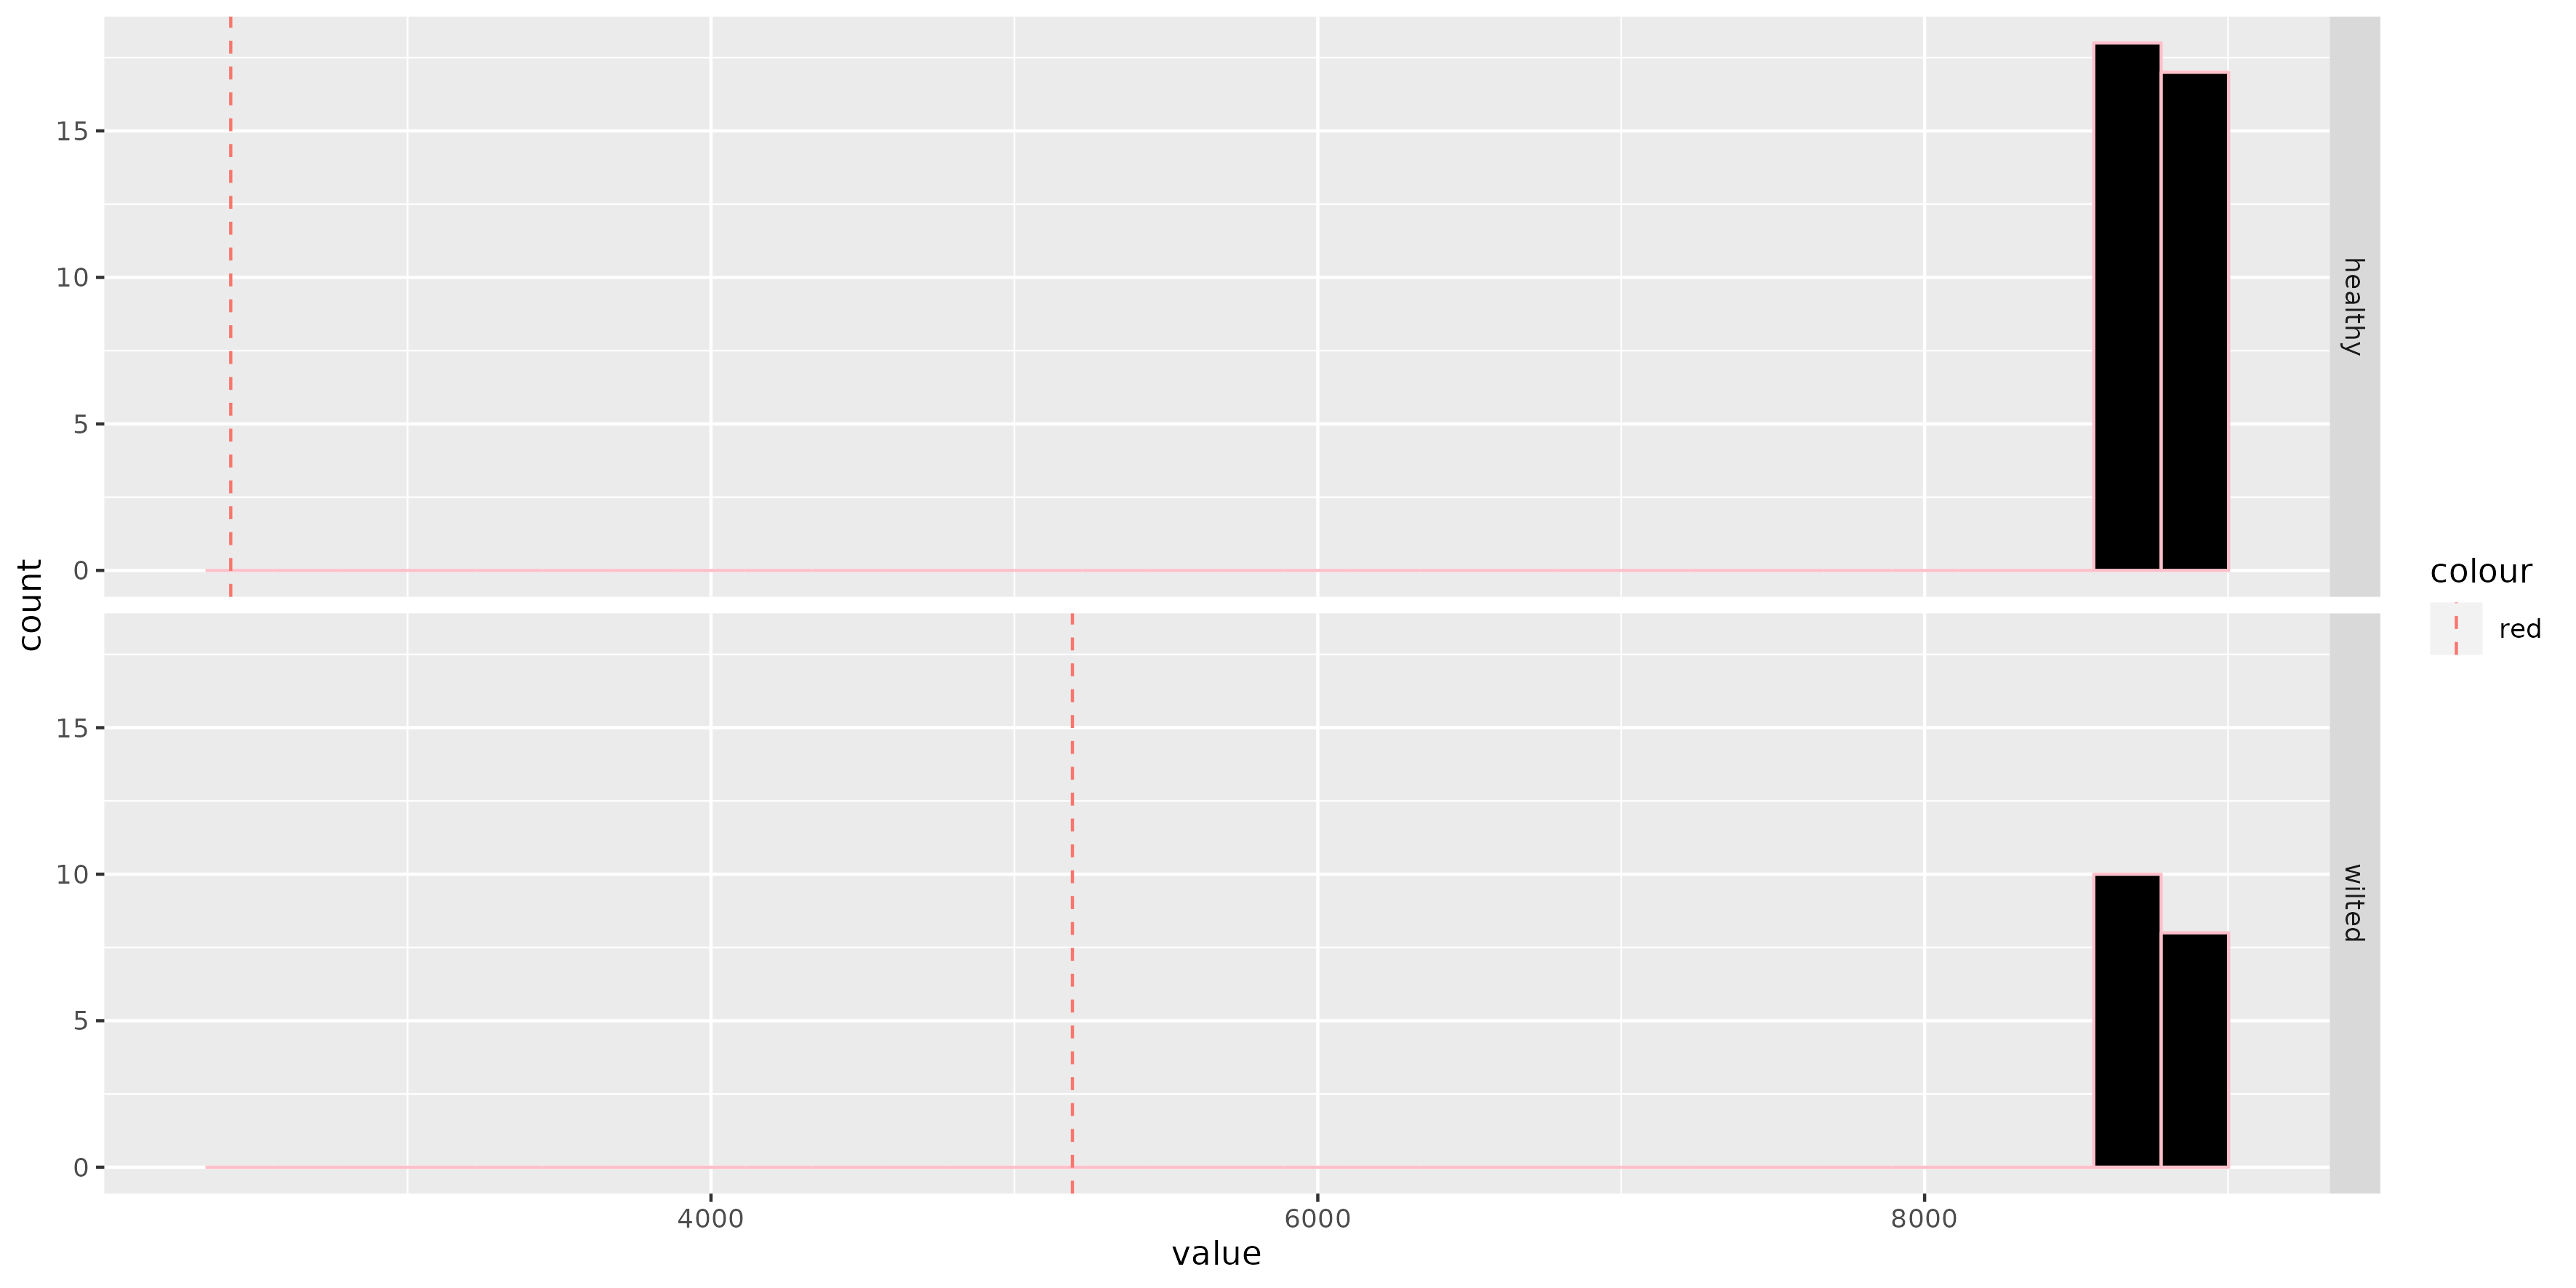
\includegraphics[width=\textwidth]{Img/cap2/varianzas_Chao1.png}
\caption{}
\end{figure}

\subsection{Prueba de los rangos con signos de Wilcolxon}

Esta es una prueba no parametrica para comparar el rango medio de dos muestras relacionadas y determinar si existen diferencias entre ellas. Se uso, ya que los datos no tienen una distribucion normal.

\begin{figure}[!]
\centering
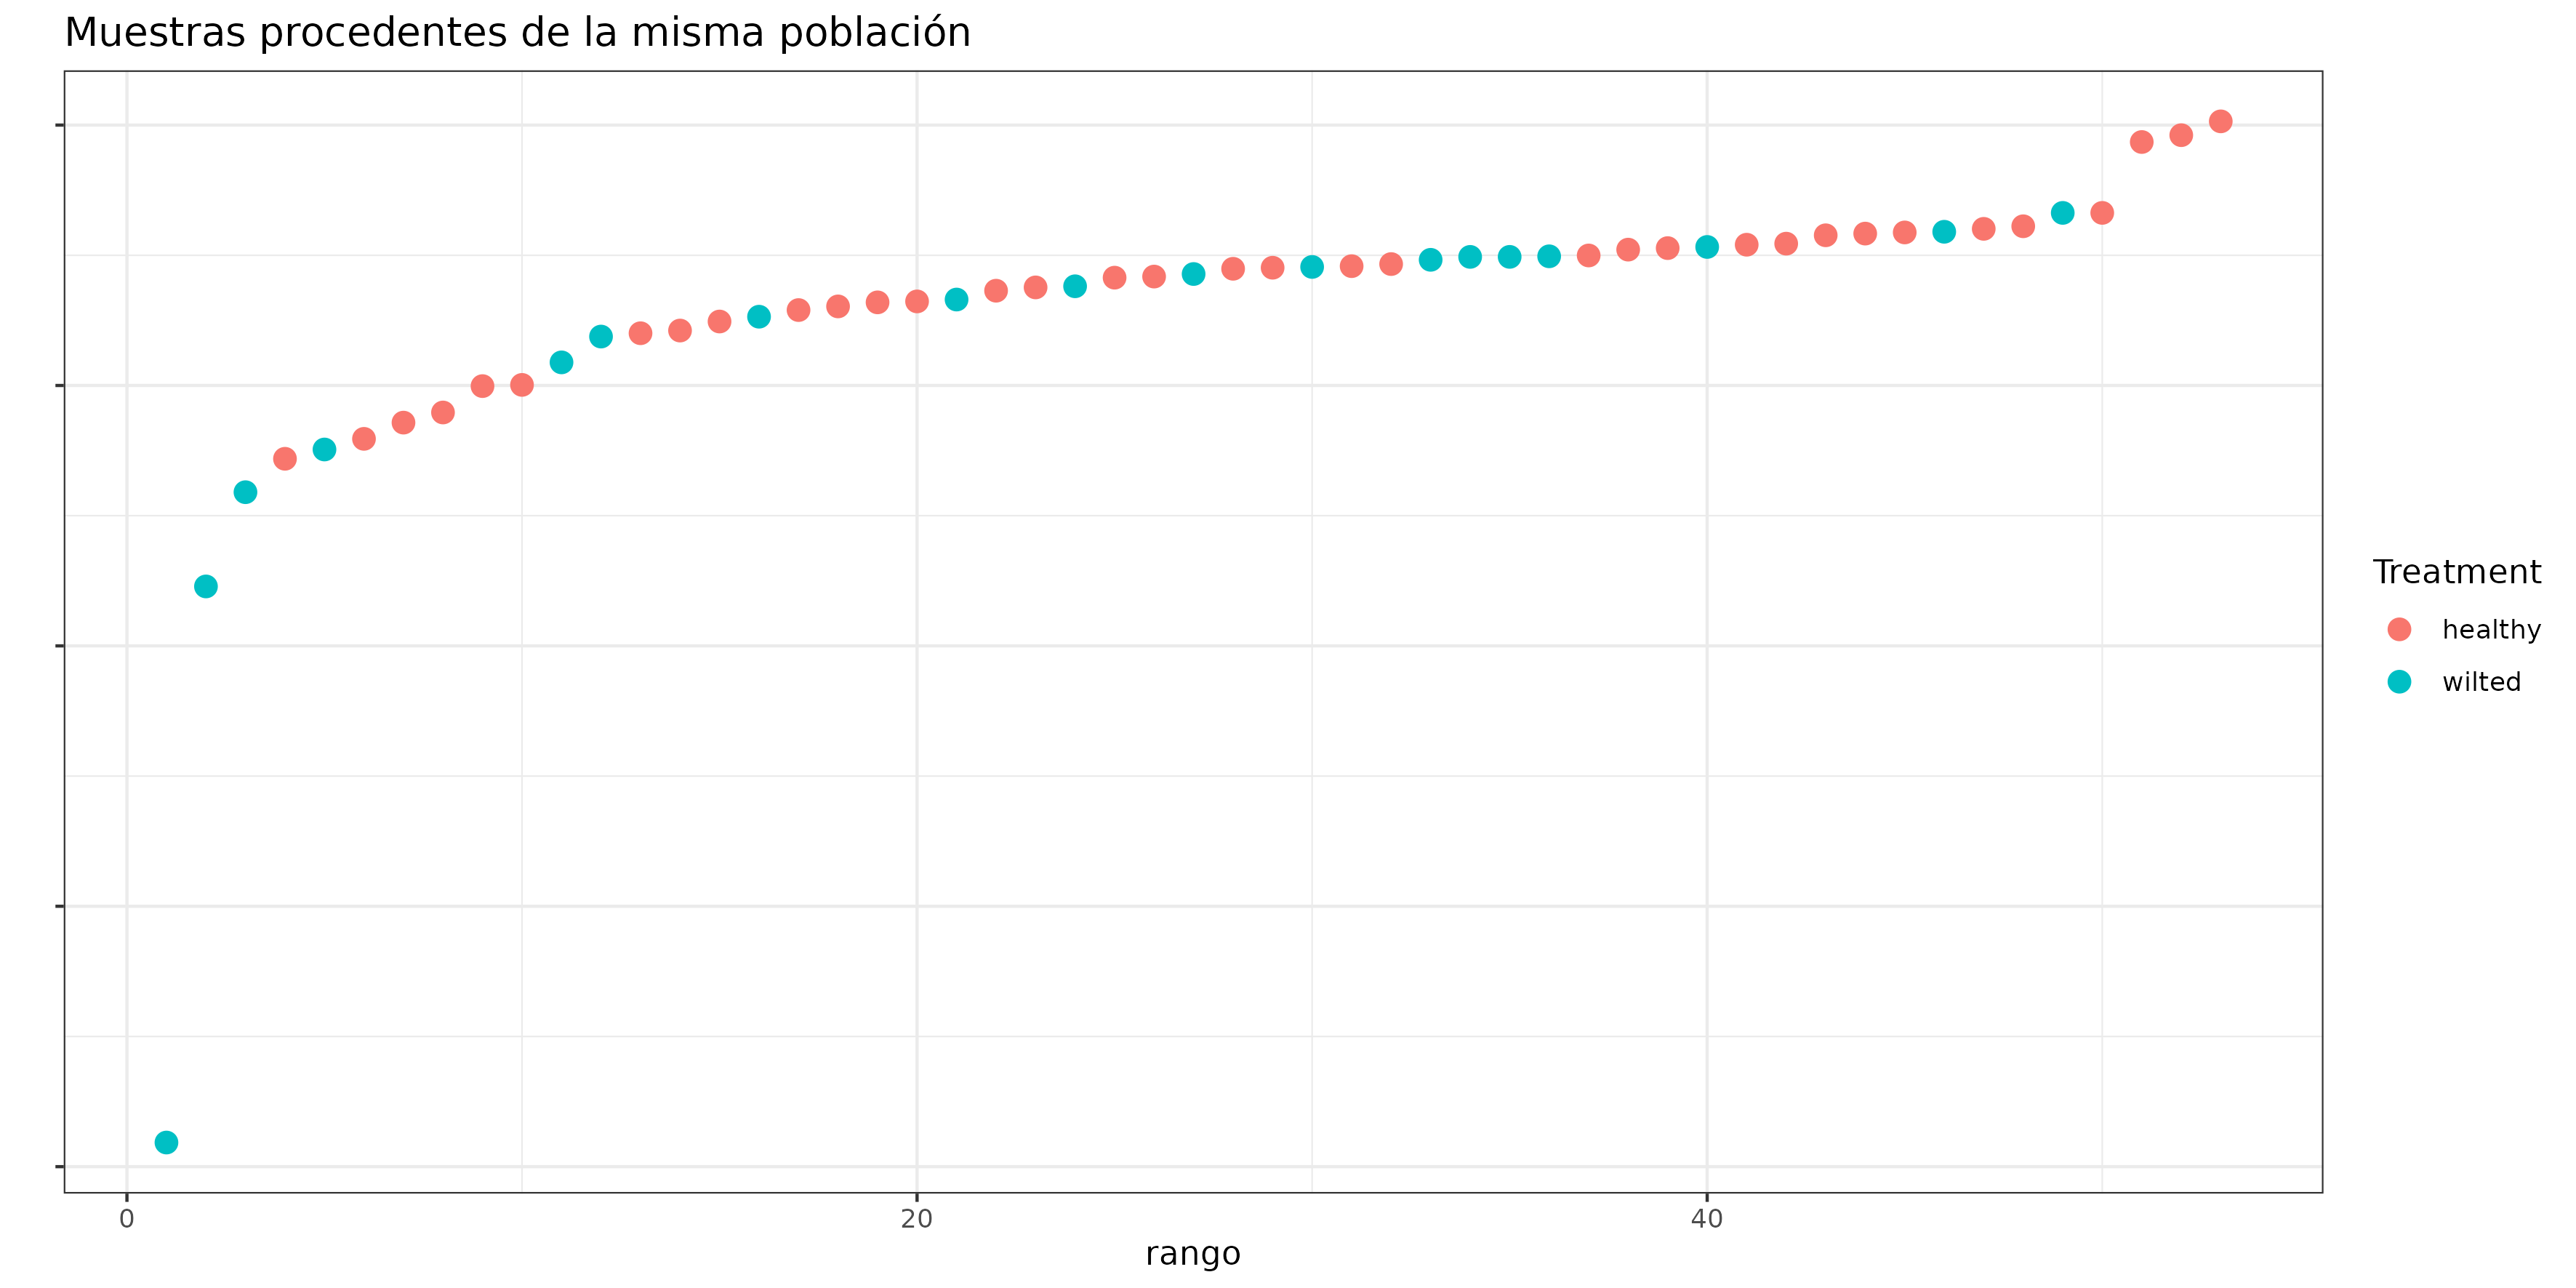
\includegraphics[width=\textwidth]{Img/cap2/Wilcoxon_Shannon.png}
\caption{Wilcoxon}
\end{figure}




Pon tu figura y describe tus resultados, y describe que es una prueba Wilcoxon


\subsection{Mann-Whitney}
La U de Mann-Whitney para comparar lasmedias dedos grupos independientes. 
Prueba no parametrica o libre de distribución, es el analogo no parametrico a la t de Student para lacomparacion de dos medias independientes; solo que esta no requiere parametros y se puede emplear sin ninguna condicion de aplicación.

\begin{figure}[!]
\centering
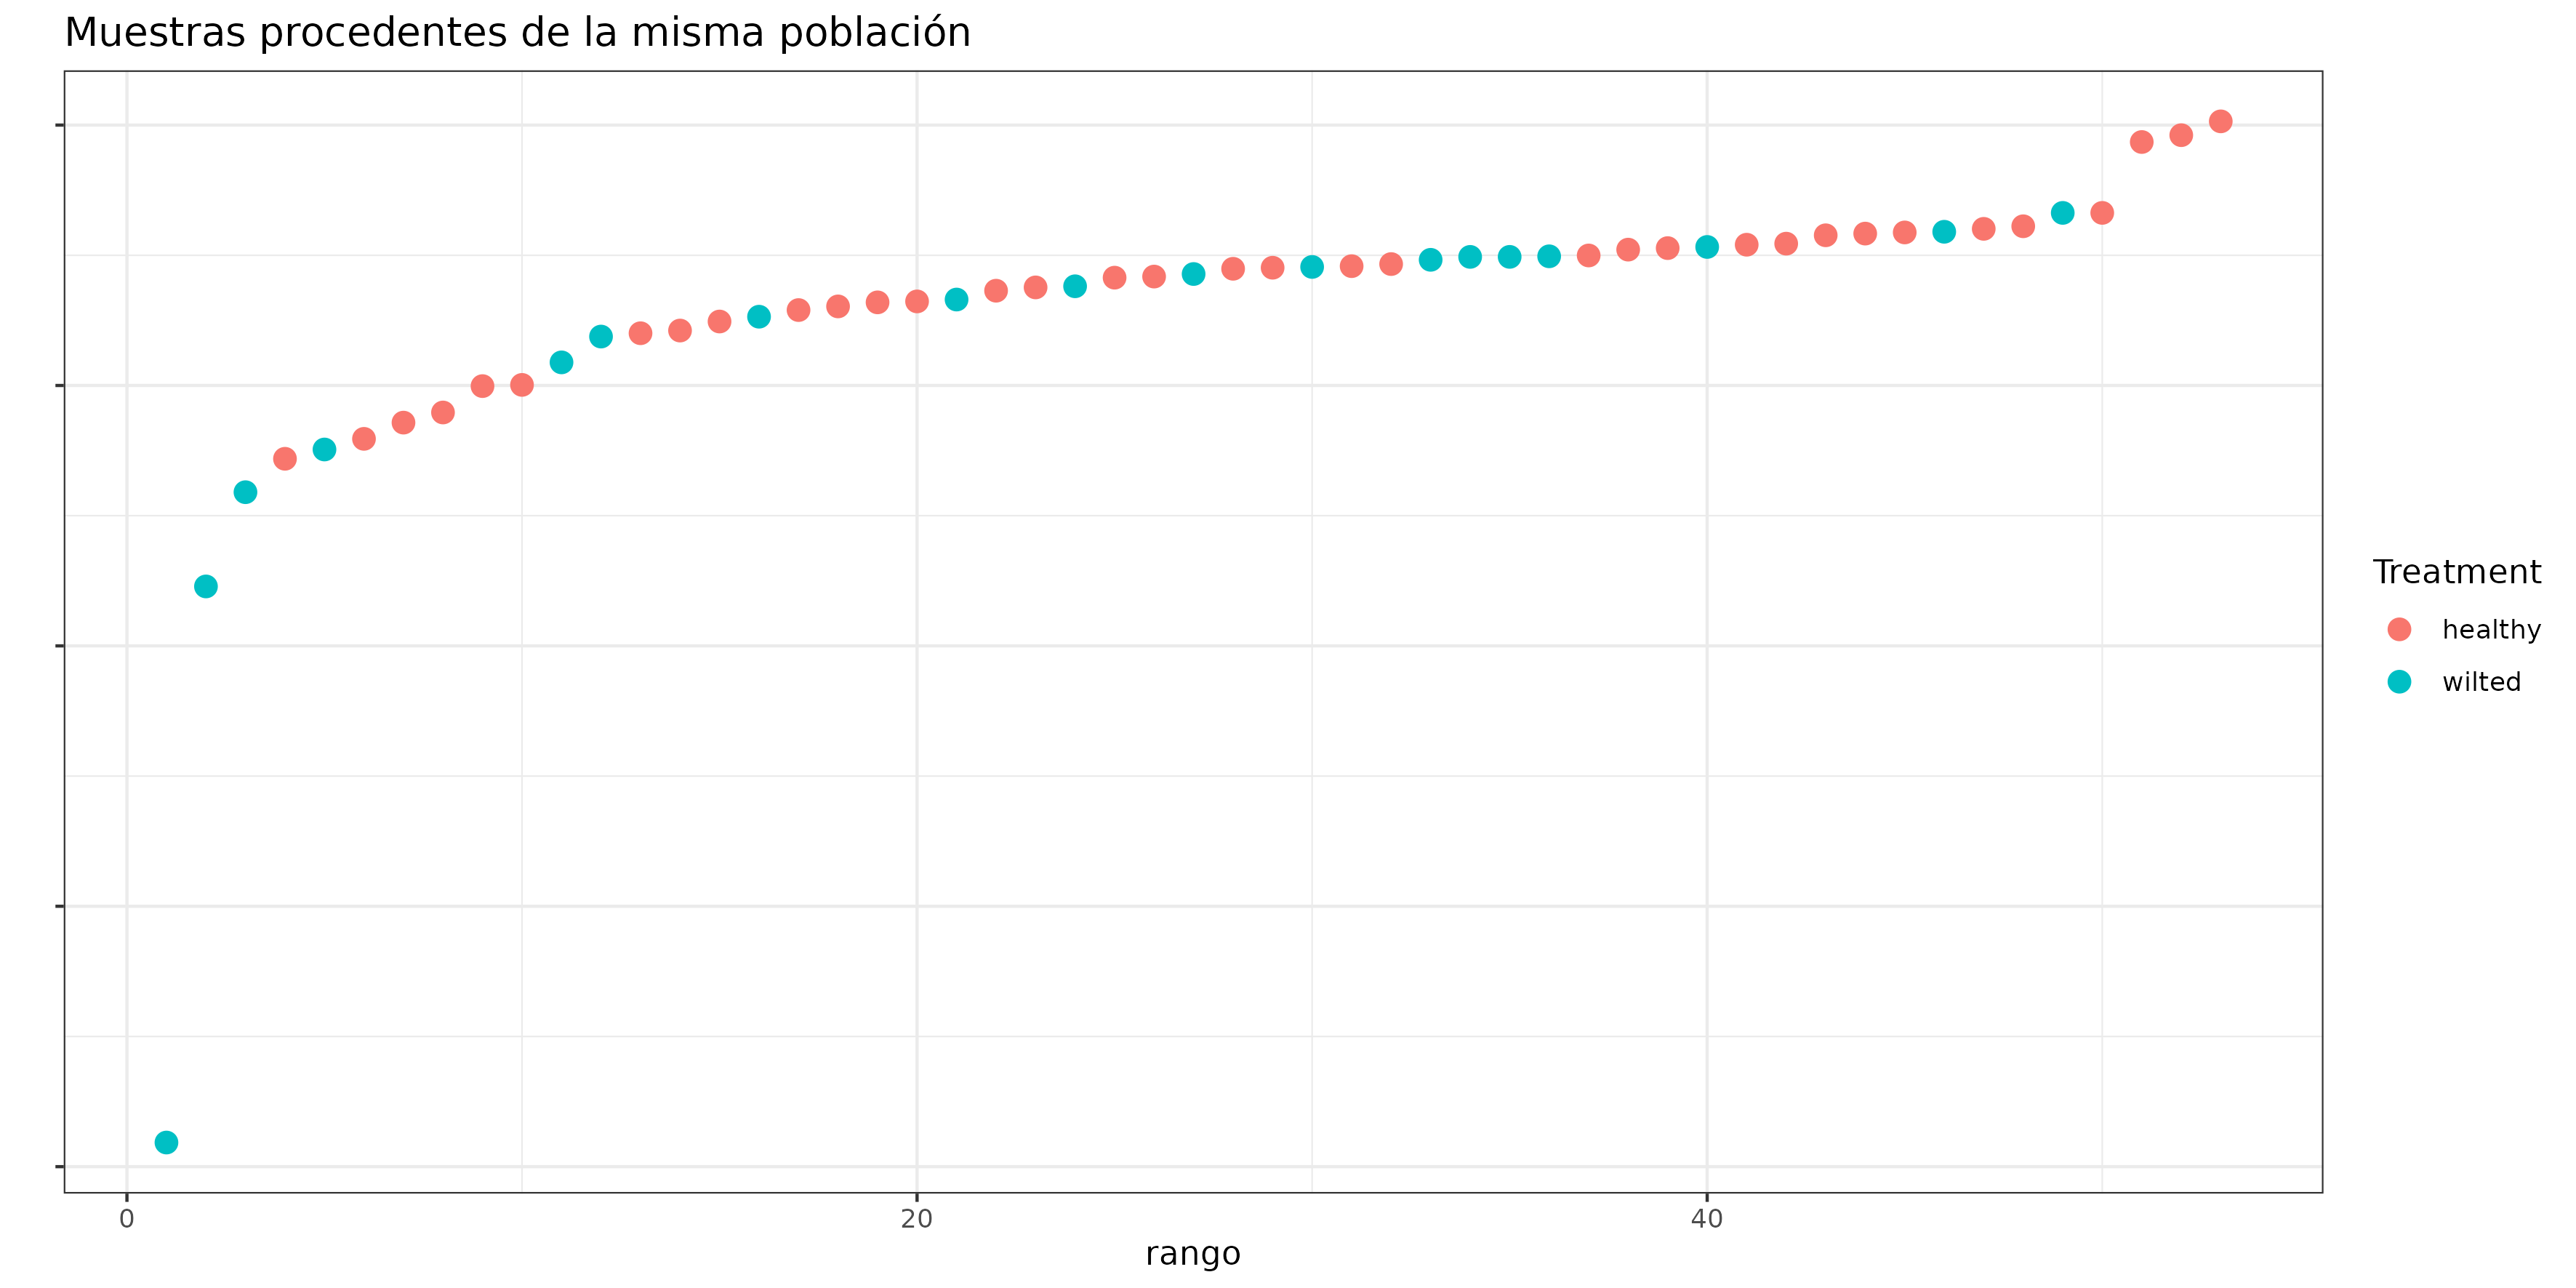
\includegraphics[width=\textwidth]{Img/cap2/Wilcoxon_Shannon.png}
\caption{Mann-Whitney}
\end{figure}



\section{Normalización}
\subsection{Normalización}

\begin{figure}[!]
\centering
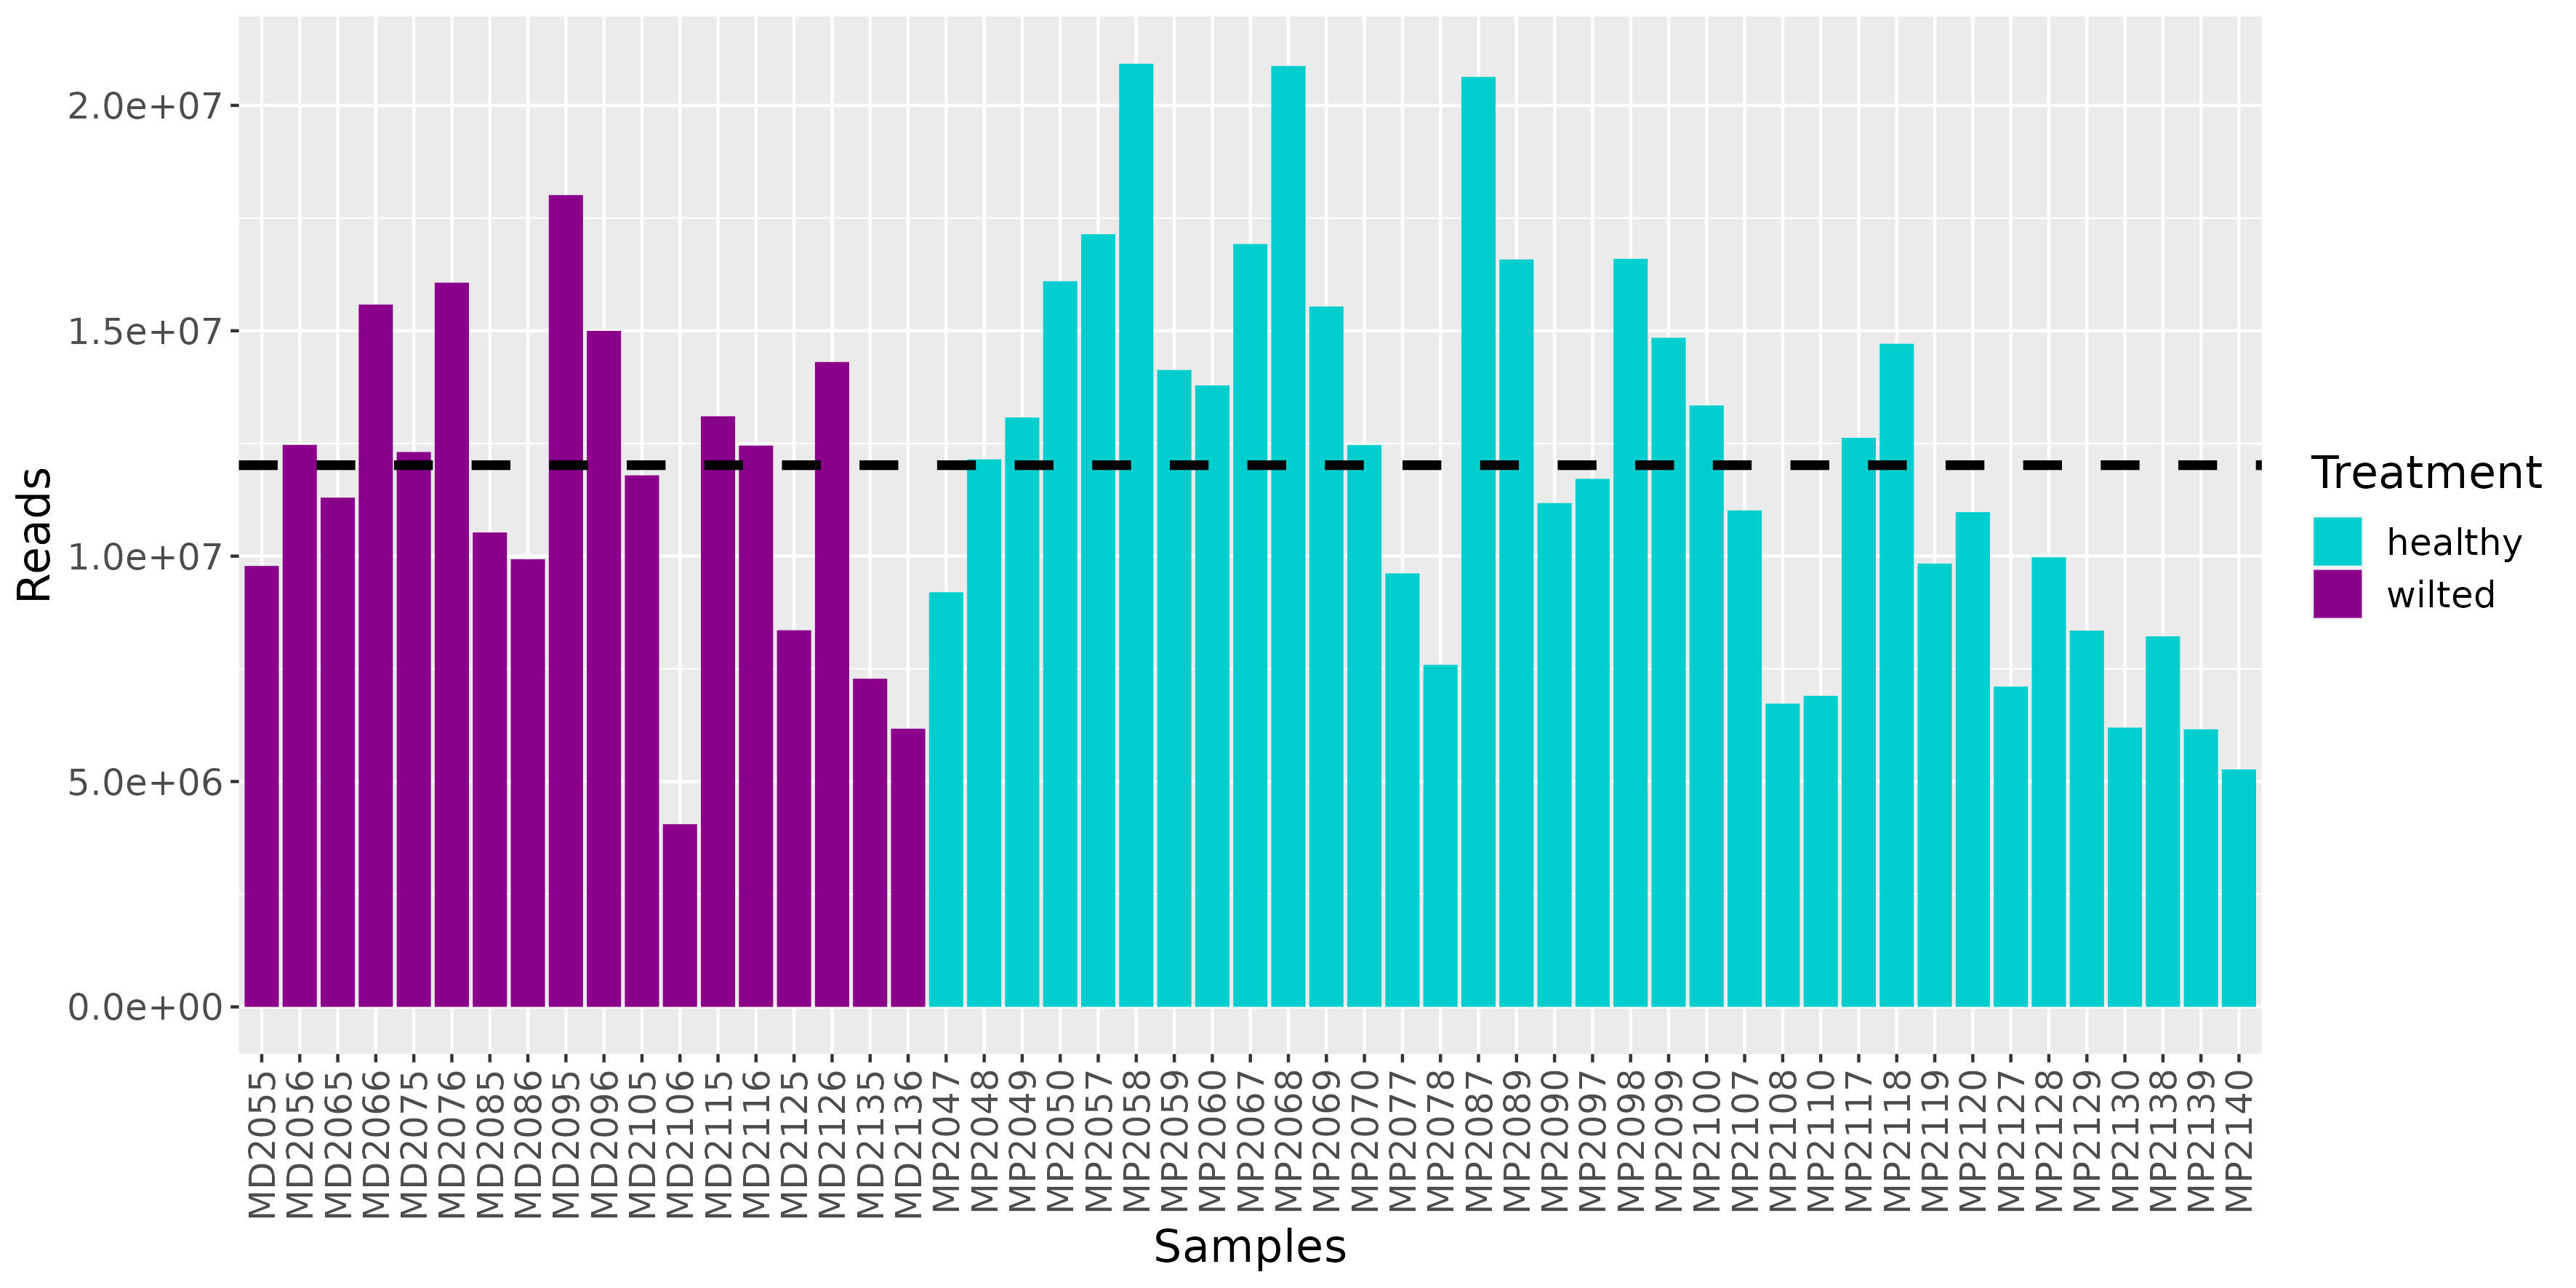
\includegraphics[width=\textwidth]{Img/cap2/Barras_Abundancia.png}
\caption{Barras de abundancia de los datos en crudo}
\end{figure}

La función edgeRnorm escala datos NGS normalizados utilizando la función de normalización provista en edgeR. Toma un objeto phyloseq y devuelve un objeto phyloseq cuya otu\_table se transforma.

\subsection{Rarefacción}
La rarefacción es una tecnica de normalización usada en el preprocesamiento de datos, para equilibrar el tamaño de las muestras en un conjunto de datos. Esta implica un submuestreo aleatorio de secuencias

Rarefy 

Se eliminaron 670 OTUs



\begin{figure}[!]
\centering
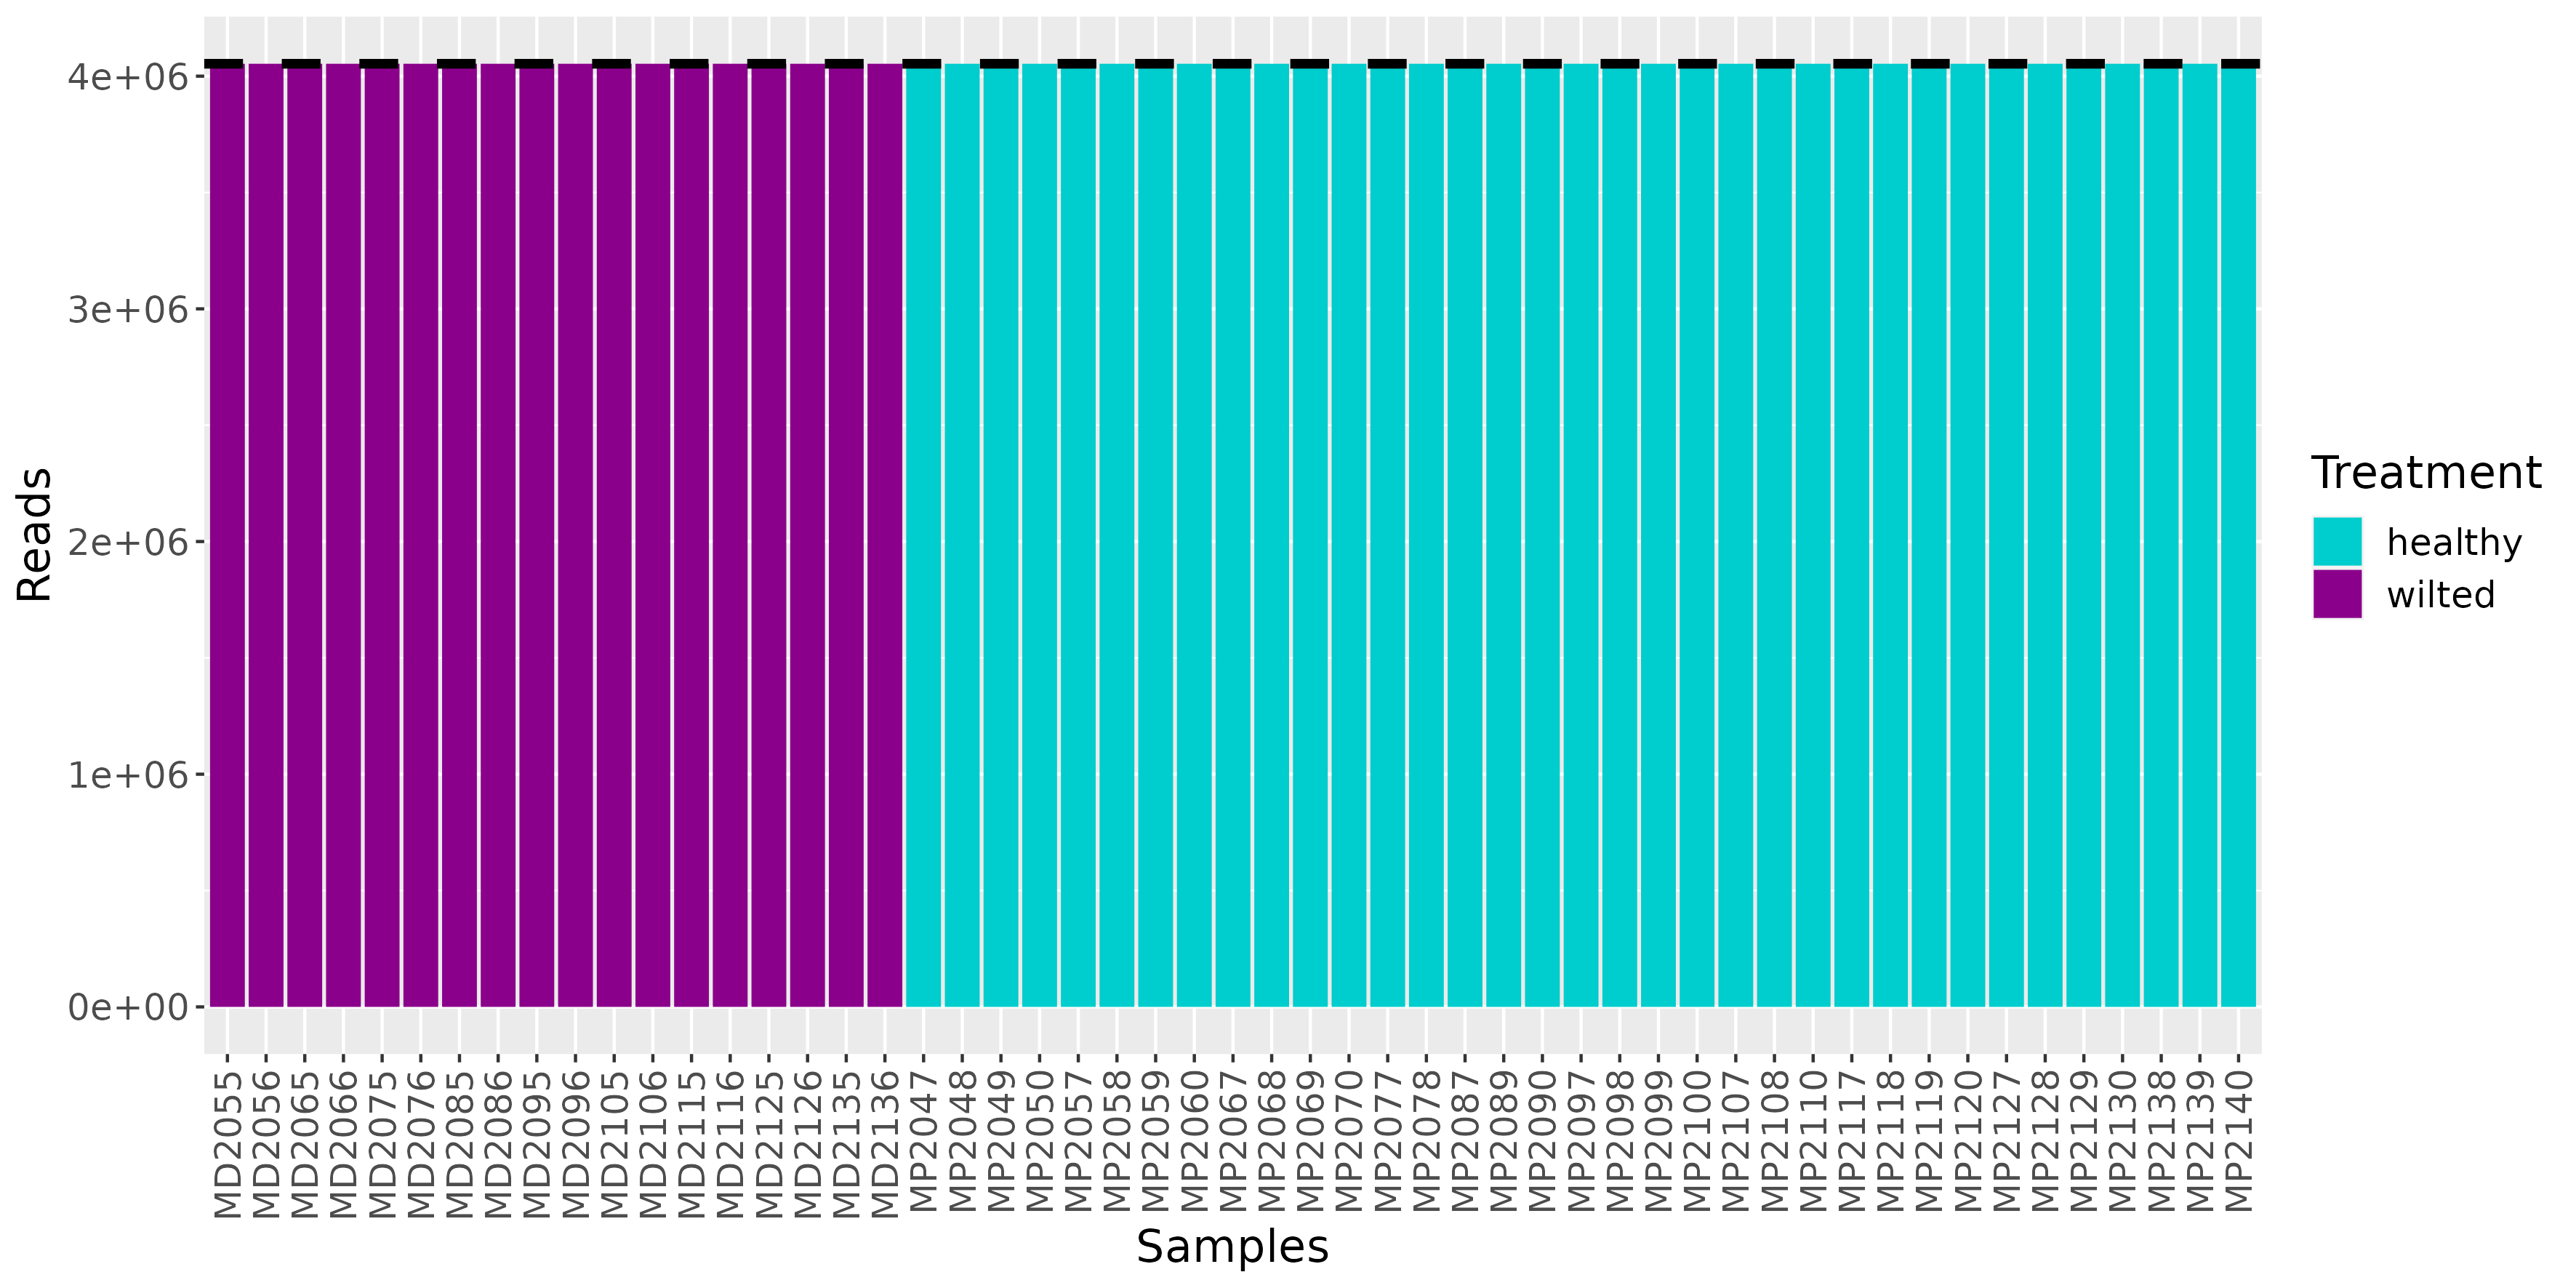
\includegraphics[width=\textwidth]{Img/cap2/Rarefaccion.png}
\caption{Barras de abundancia, luego de la rarefacción}
\end{figure}

\begin{figure}[!]
\centering
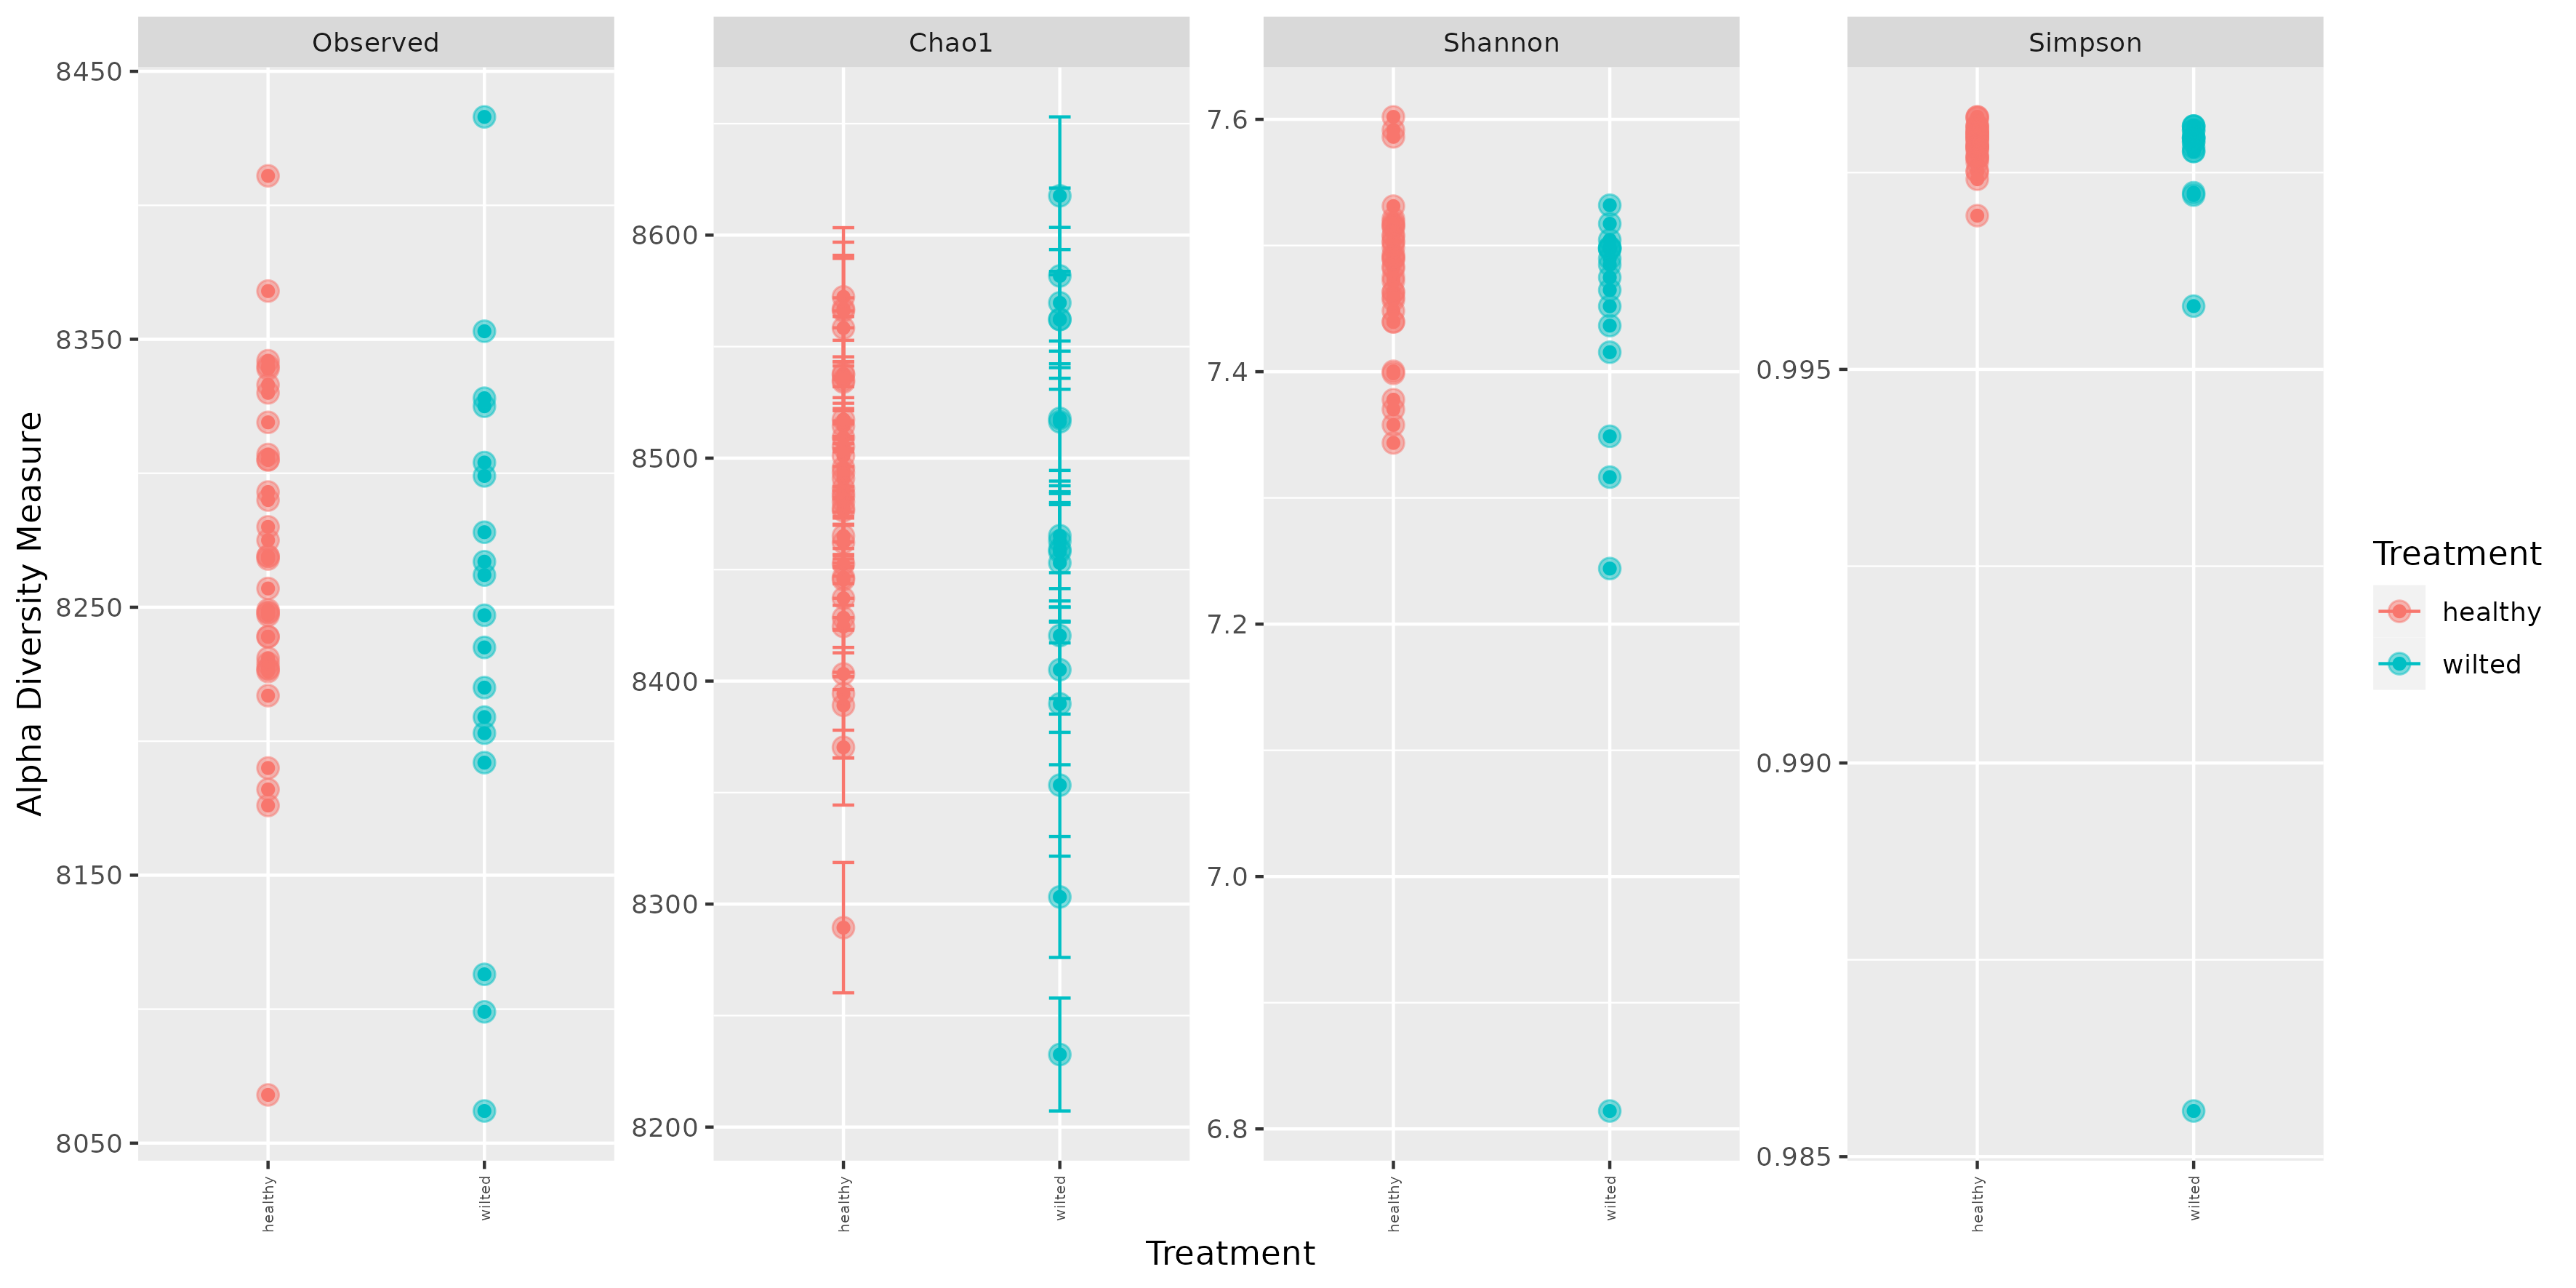
\includegraphics[width=\textwidth]{Img/cap2/Rarefaccion_diversidadAlfa.png}
\caption{Diversidad alfa luego de la rarefacción}
\end{figure}

\begin{figure}[!]
\centering
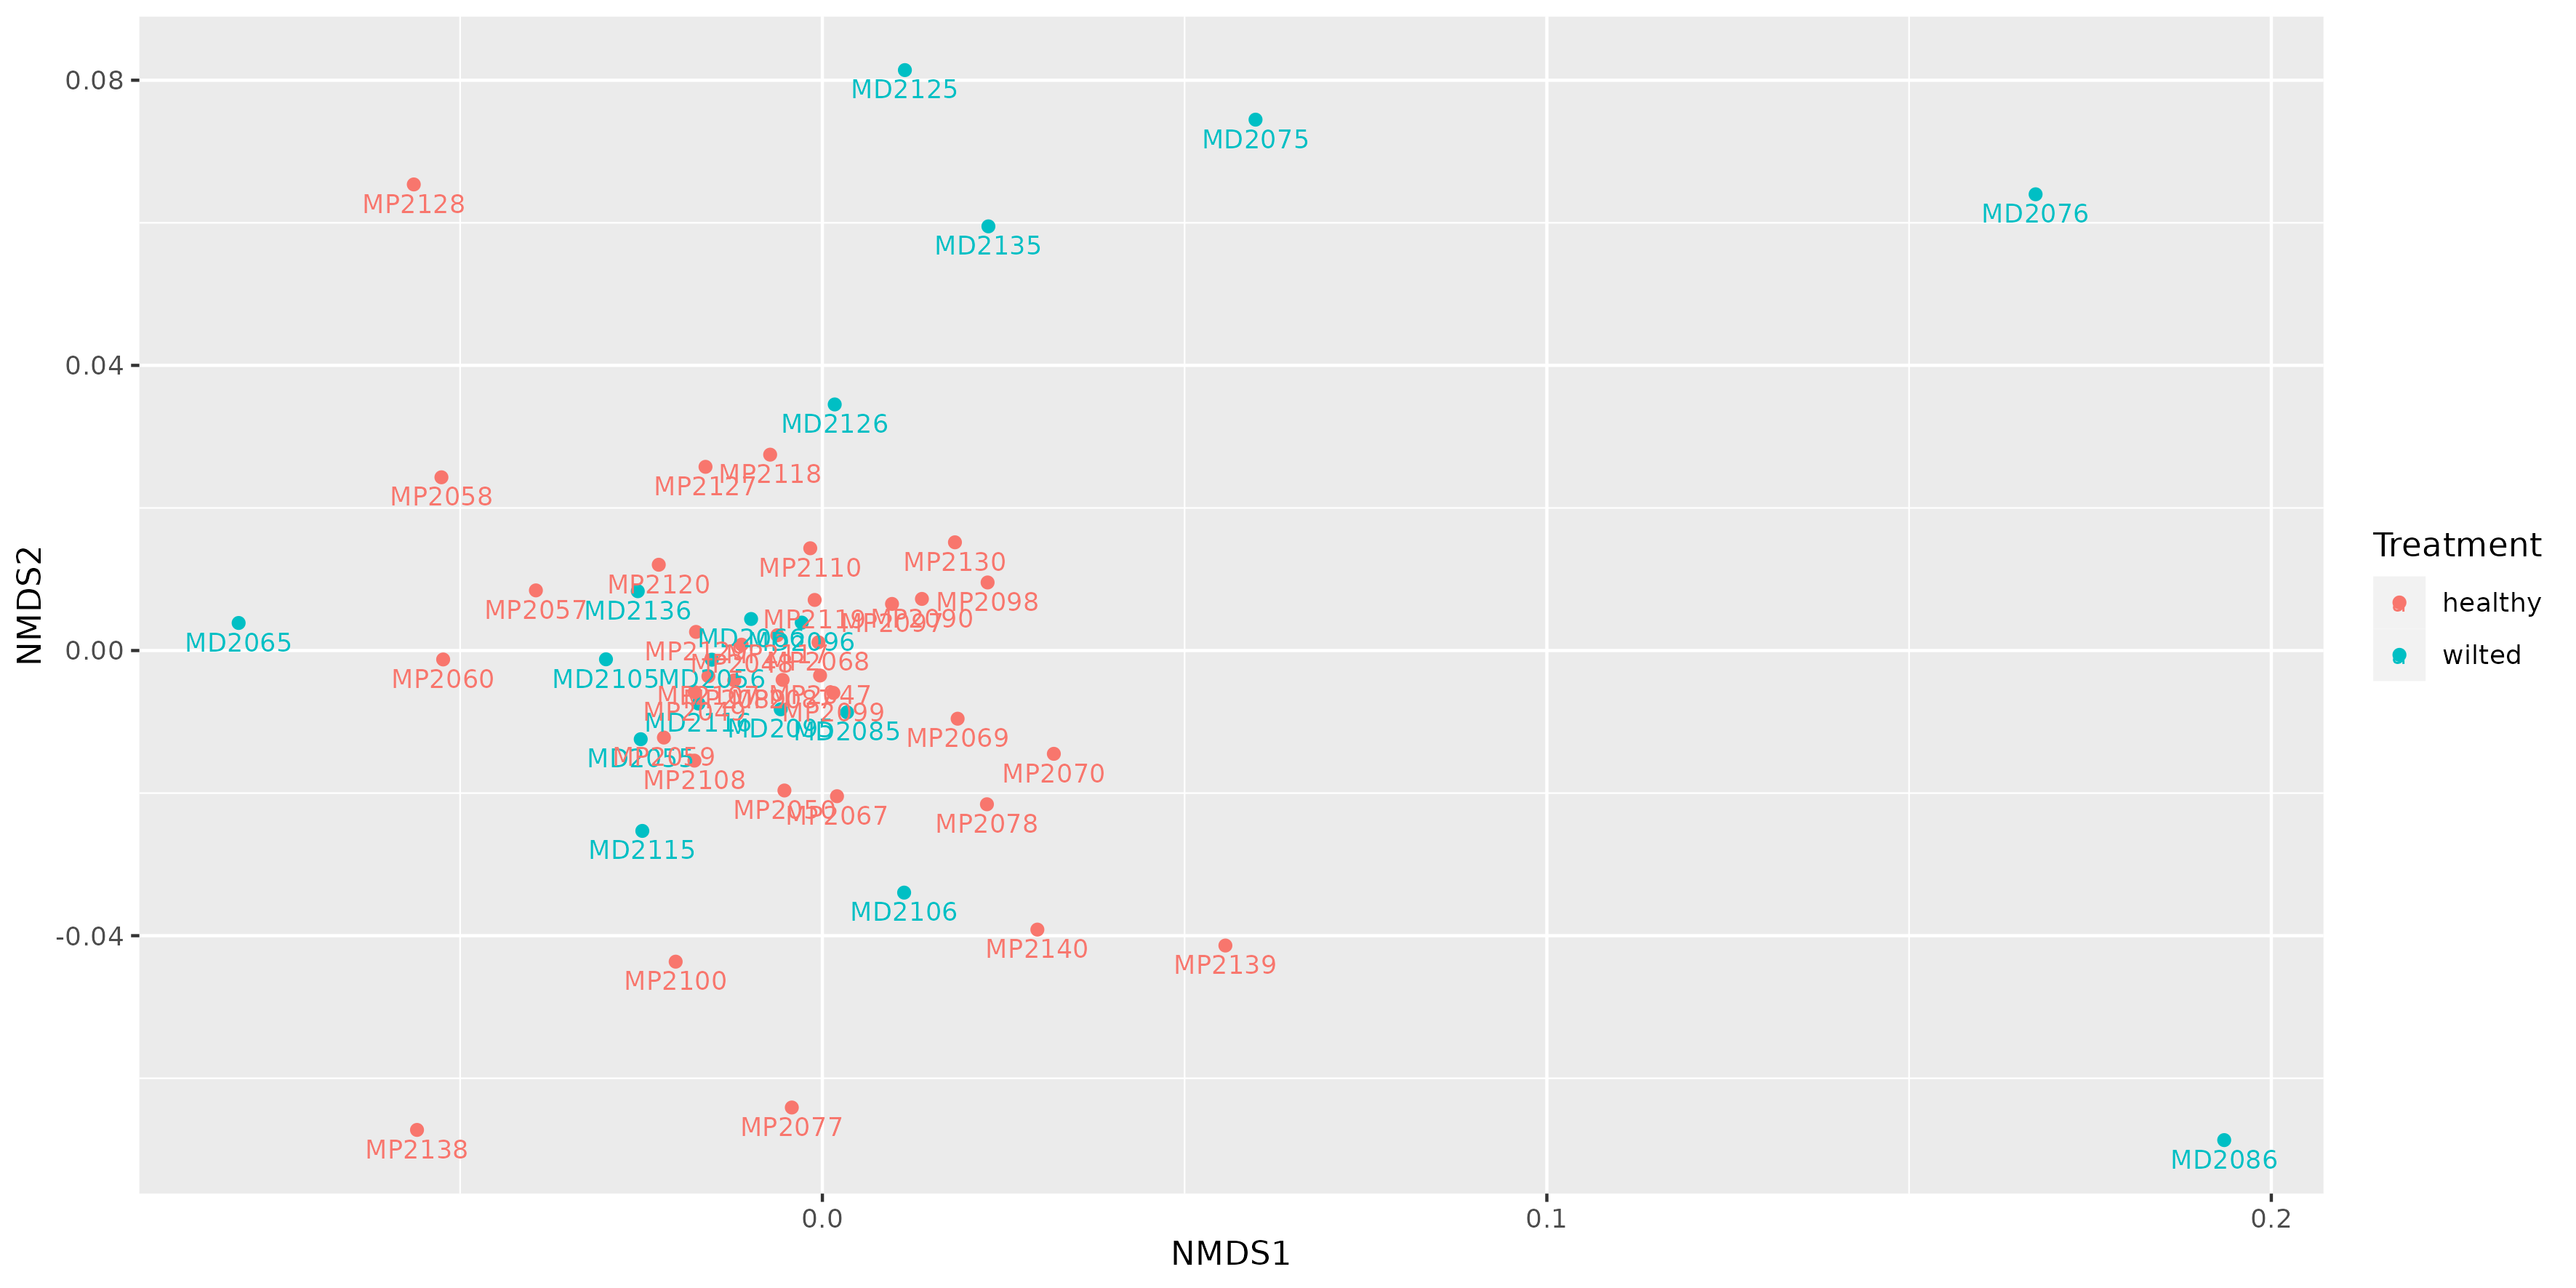
\includegraphics[width=\textwidth]{Img/cap2/Rarefaccion_diversidadBeta.png}
\caption{Diversidad beta luego de la rarefacción}
\end{figure}

\section{Rarefacción}
La rarefacción se usa como una medida de saturacion de muestras, es decir, 




\section{Redes}





Para poder visualizar las redes de nuestros datos, podemos hacer un data.frame uniendo toda la informacion
del objeto phyloseq.\\

\begin{lstlisting}
    df <- psmelt(fresa_kraken_fil)
\end{lstlisting}

Hay dos funciones en el paquete phyloseq para trazar la red del microbioma usando “ggplot2”: plot\_network() y plot\_net().
Se crea un grafo basado en “igraph”, basado en el método de distancia por defecto, Jaccard y una distancia
máxima entre nodos conectados de 0,8. El “Treatment” se utiliza para los mapeos de color y forma para
visualizar la estructura de las muestras.

Hacemos un grafo a partir de el objeto phyloseq

\begin{lstlisting}
    ig <- make_network(fresa_kraken_fil, max.dist=0.8)
\end{lstlisting}

Y luego lo graficamos.

\begin{lstlisting}
    plot_network(ig, fresa_kraken_fil, color="Treatment", shape="Treatment")
\end{lstlisting}

\textbf{INSERTAR AQUI IMAGEN DEL GRAFO}

En este grafo podemos ver la complejidad de los datos y las conexiones entre nuestras muestras.\\

En comparacion con la función plot\_network(), la nueva función plot\_net() no requiere una llamada separada a la función make\_network(), o un objeto igraph separado. Los siguientes códigos crean una red basada en una distancia máxima entre los nodos conectados de 0,5.

\begin{lstlisting}
    plot_net(fresa_kraken_fil, maxdist = 0.5, color = "Treatment", shape="Treatment
\end{lstlisting}

\textbf{INSERTAR AQUI IMAGEN DEL GRAFO}

En conclusion para esta observación general de los datos, no es posible ver una separacion entre muestras
sanas y enfermas claramente con la diversidad beta,y con los graficos de barras y redes, no es posible
identificar datos especiales.




\textbf{PONER GRAFOS Y DATOS DE REDES HECHAS CON FONTY}

Luego de una breve visualizacion de redes simples, tenemos dos opciones para utilizar ls redes de coocurrencia

El analisis de co-ocurrencia utiliza la matriz de interacciones
Redes de co-ocurrencia - El total de nodos de la red es el numero de OTU's en una tabla; se quiere ver las relaciones entre nodos. LAs aristas representan co-ocurrencia entre de nodos.

MicNet - Microbial Network
Esta herramienta nos pide un documento BIOM (la tabla de abundancias) en formato .csv para poder entregar las matriz de correlaciones usando normalizacion de Dirichlet, esta herramienta se divide en tres: 
UMAP - Cluster - Este algoritmo permite ver los datos en el plano.
Sparcc - Matriz de correlación
Network - pide los dos anteriores y genera la red completa

Redes en Alnitak
Esta herramienta calcula los vecinos de un taxon especifico contra el resto de los taxones, midiendo el taxon de interes con dos metricas diferentes.
Aqui pide el documento BIOM cortado por nivel taxonomico del taxon escojido, junto con el TaxID del mismo; entregando una matriz de correlaciones filtrada por el taxon de interes, que solo reporta las correlaciones con el taxon escojido al nivel taxonomico tomado, que pasen los umbrales de correlacion mayor a un 0.7 y disimilitud de bray curis menor a un 0.3. 
Asi la primera red creada con esta herramienta es tomando Fusarium a nivel de genero, ya que como se vio anteriormente es un genero importante entre los datos de Eucariota…





\section{Rs}

Se obtuvo un nuevo conjunto de datos complementario, el cual se divide en cinco categorias, respecto al tipo de cultivo de las fresas,

\begin{figure}[!]
\centering
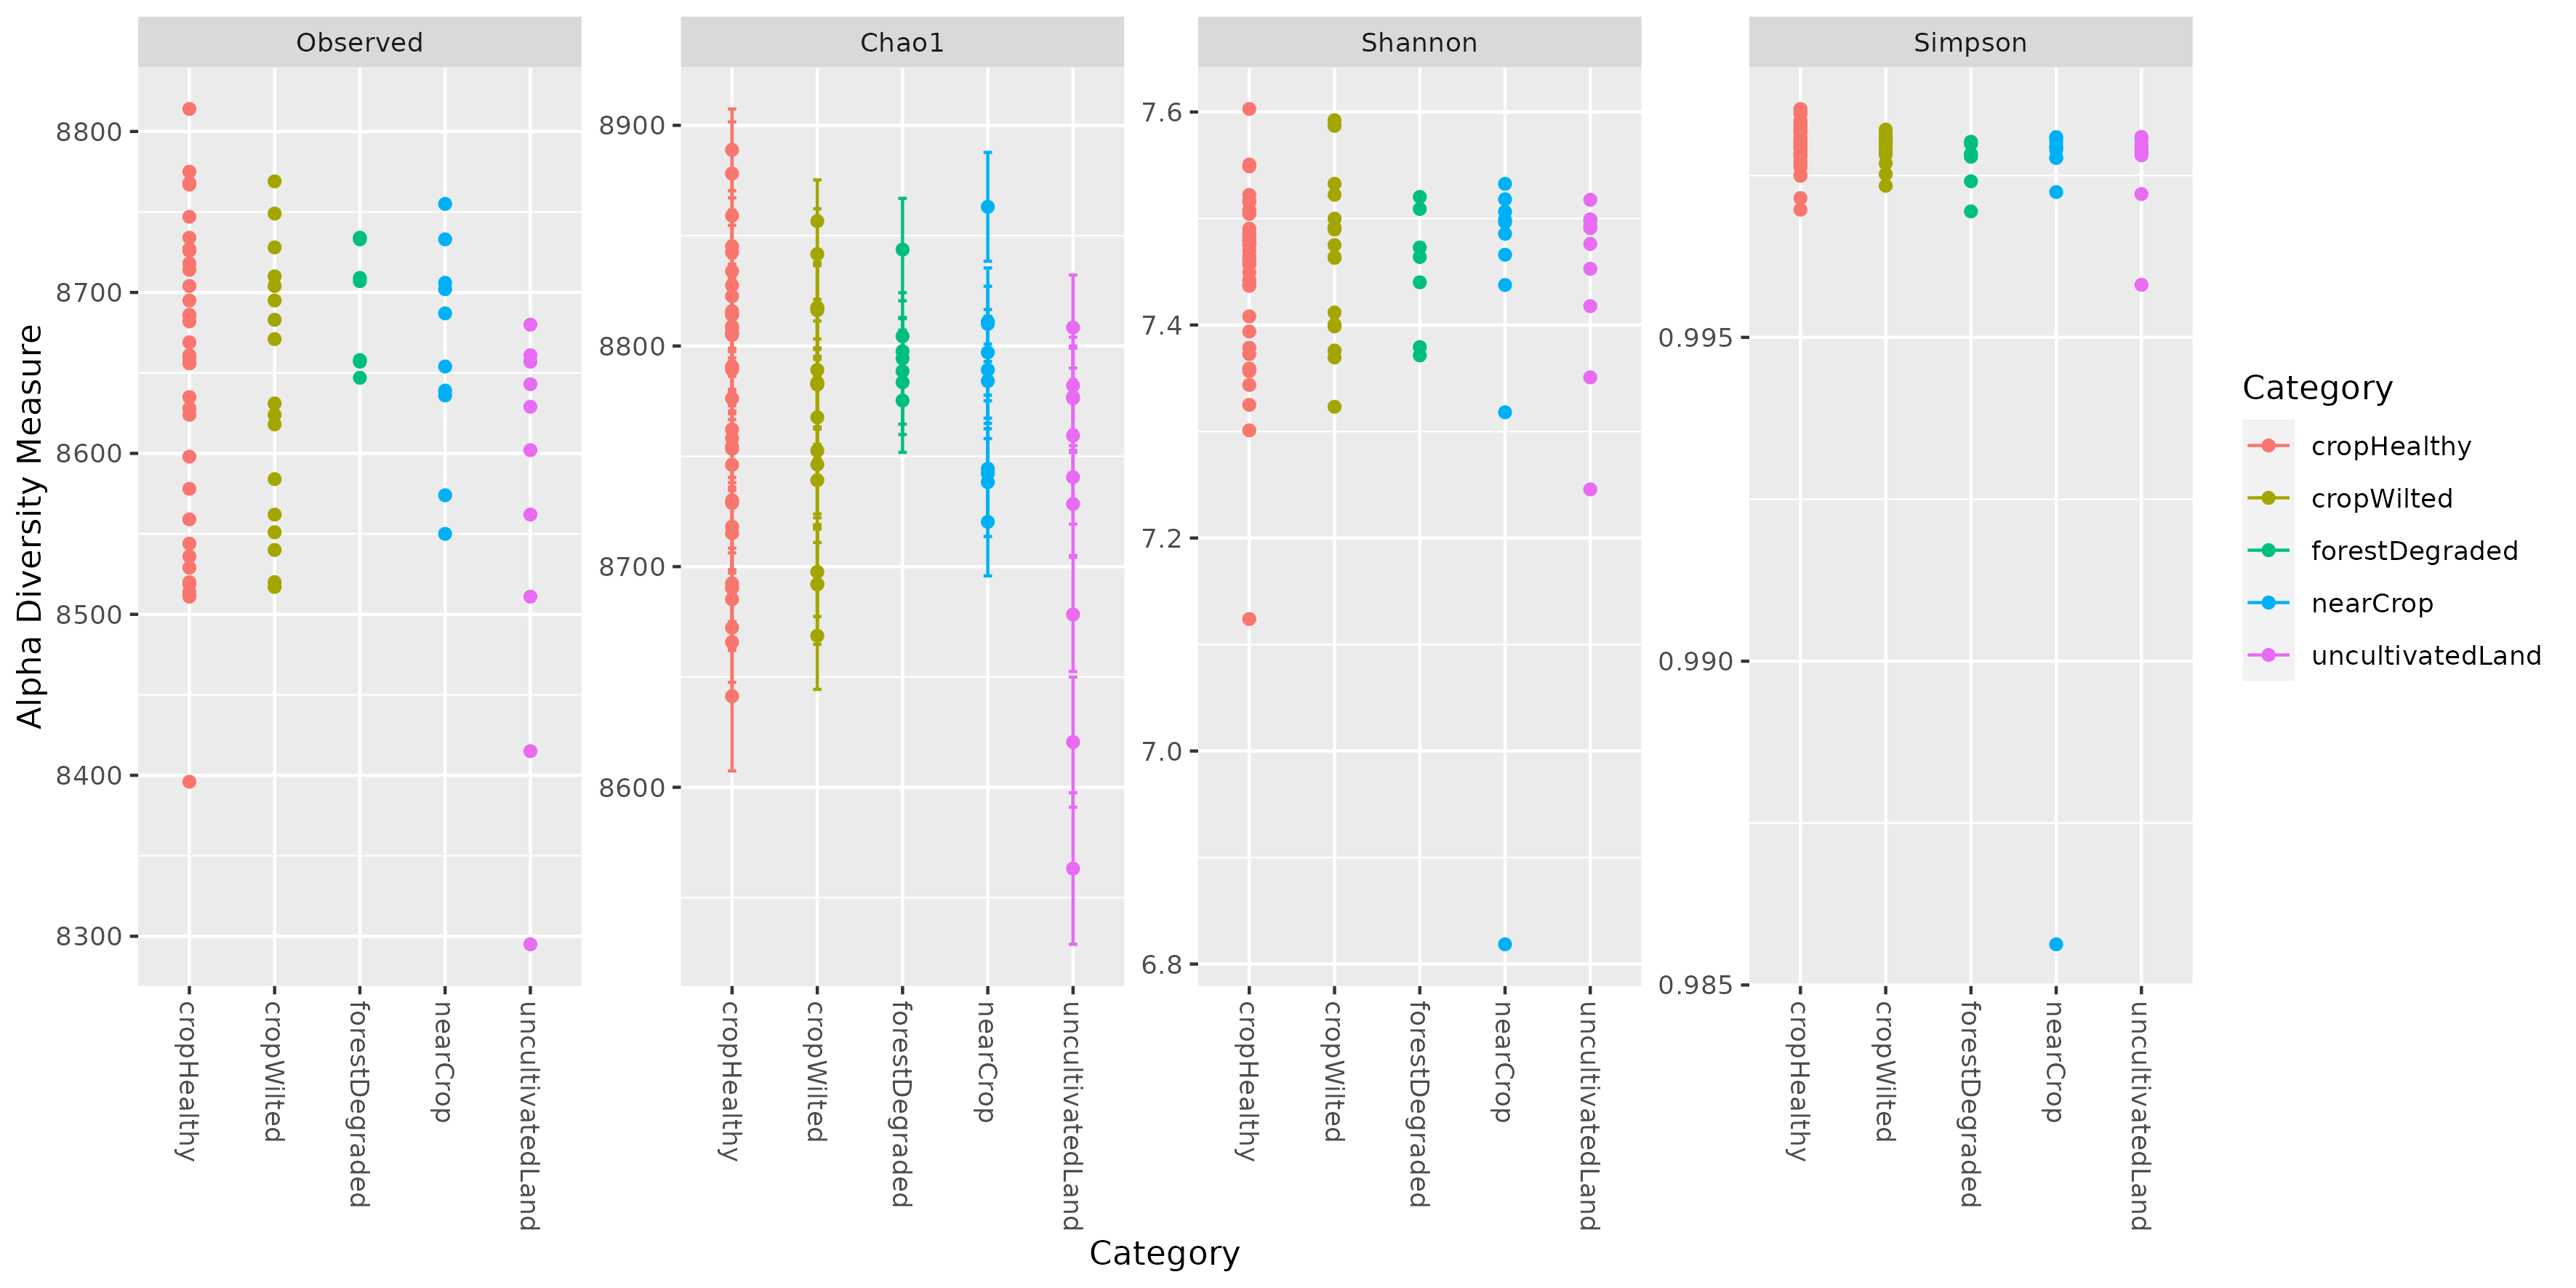
\includegraphics[width=\textwidth]{Img/cap2/AllData_Alfa_diversidad.png}
\caption{Diversidad Alfa, }
\end{figure}

\begin{figure}[!]
\centering
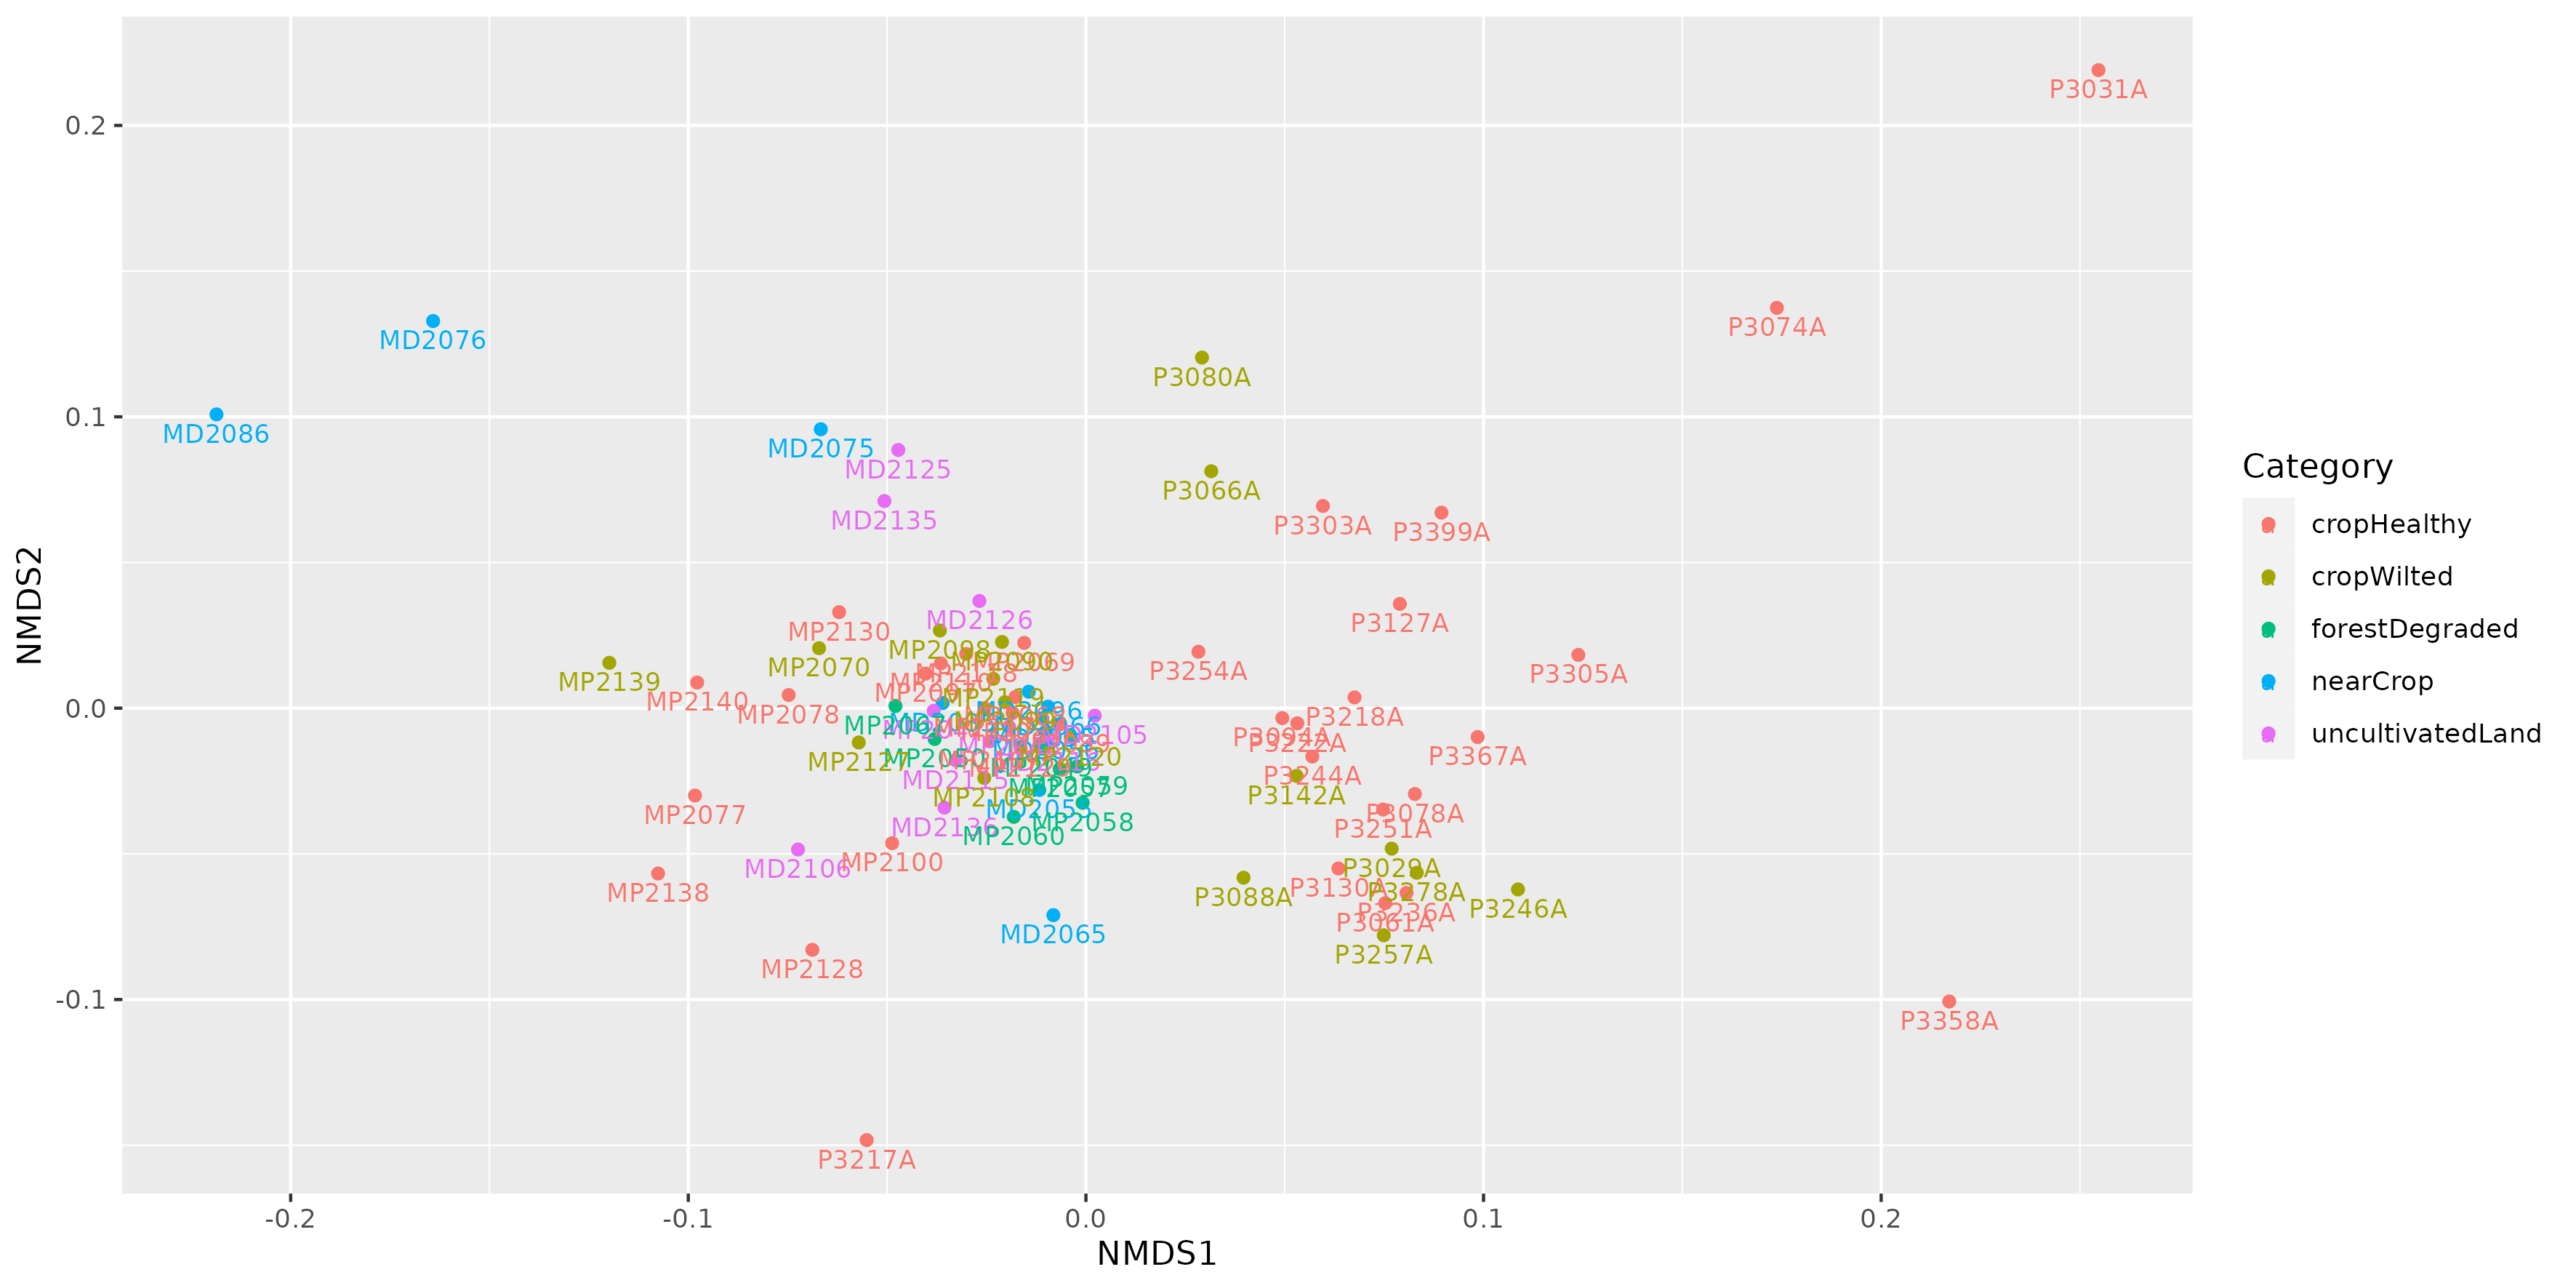
\includegraphics[width=\textwidth]{Img/cap2/AllData_Beta_diversidad.png}
\caption{Diversidad Beta, }
\end{figure}
\thispagestyle{empty}

\chapter{Simulador Metagenómico PyMetaSeem}
Un problema abierto en la metagenómica es distinguir la calidad del ensamblaje y la correcta asignación taxonómica de los datos metagenómicos. Para lo cual es necesario tener datos metagenomicos de referencia de calidad, que contengan un sistema de clasificacion de la calidad de estos datos debidamente clasificados taxonomicamente, y de alta calidad para poder realizar la evaluacion de las herramientas de software de clasificación taxonomica y  de ensamblaje. Por esto se han realizado distintos simuladores de datos metagenomicos, los cuales se revisan en este capitulo, llegando a la conclusión de que la gran mayoria tienen complicaciones para su uso, y asi empezaremoscon la creaccion de nuestro propio simulador de datos metagenomicos.   \\

%\begin{figure}[h]
%\centering
%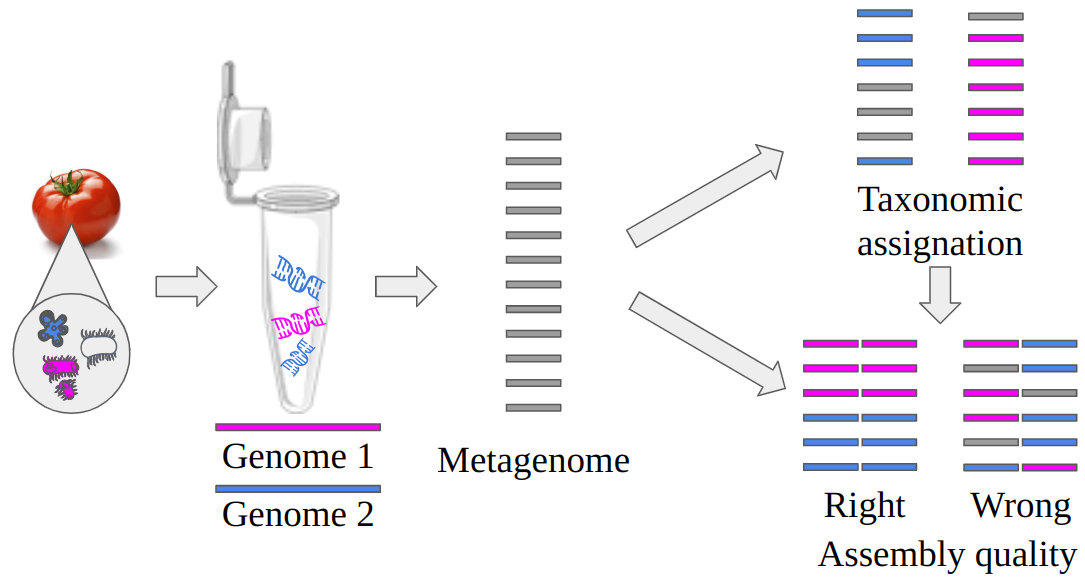
\includegraphics[width=\textwidth]{Img/cap2/problem.png}
%\caption{Flujo }
%\end{figure}


\section{PyMetaSeem: simulador de datos metagenómicos a partir de un conjunto de datos genómicos}

PyMetaSeem es un algoritmo creado desde cero que simula datos metagenómicos a partir de datos genómicos. Este simulador de datos metagenómicos fue creado a partir de reads recortadas de datos genómicos. Los genomas reales se utilizan para calificar la precisión de los clasificadores y ensambladores taxonómicos. Está pensado como un entorno conda, escalable, reproducible, fácil de usar y gratuito para el público ya que otros simuladores conocidos (como CAMISIM) tienen dificultades de instalación e implementación.  \\


%\begin{figure}[h]
%\centering
%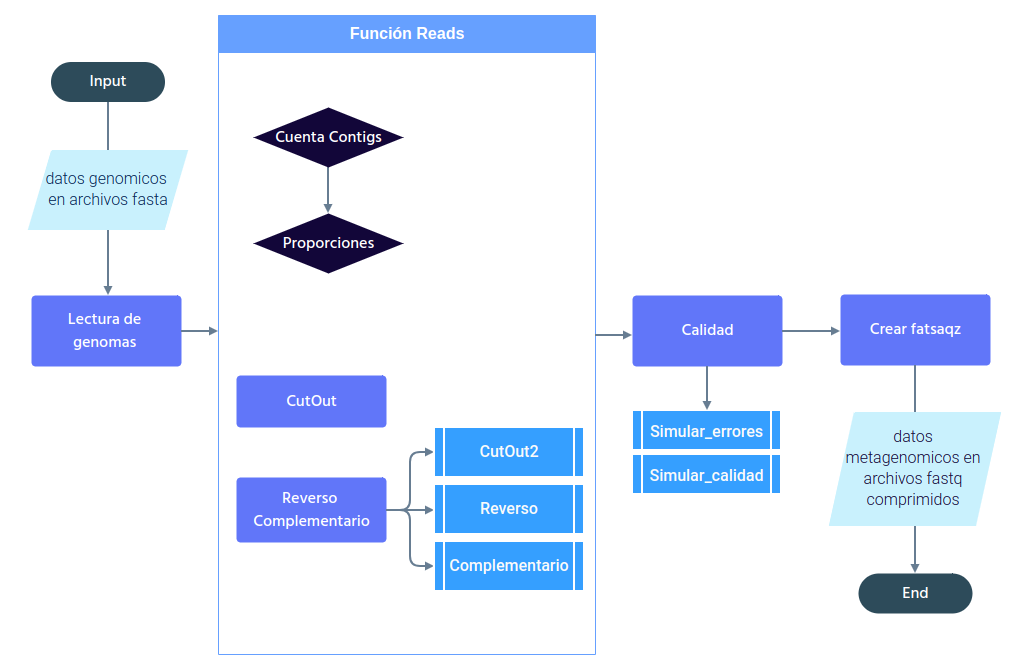
\includegraphics[width=\textwidth]{Img/cap2/diagrams_de_flujo.png}
%\caption{Diagrama de Flujo PyMetaSeem}
%\end{figure}

Este algoritmo está compuesto de varias funciones:

PyMetaSeem recibe un conjunto de archivos con diferentes genomas en formato FASTA, para esto se tienen las opciones de inicializar el algoritmo con numero de reads y longitud de reads ya sea manual o en un archivo de texto (txt) que contenga elnombre de los archivos y la cantidad de reads por genoma (perfil taxonomico).  \\

Se tiene una función que se encarga de de la lectura de los fasta, convirtiendolos en un diccionario que contiene cada secuencia de nucleótidos como valor y su nombre o identificador como clave, lo que facilita la gestión de los datos dentro de python.   \\

Teniendo los genomas en diccionarios, se crean varias funciones para tomar las longitudes de los reads a recortar y las proporciones,  tomando en cuenta el tamaño original de los contigs. Luego de obtener las longitudes y proporciones, se cortan los reads aleatorias (m) de una longitud determinada (n) a partir de la secuencia de nucleótidos.  \\


\subsection{Simulaciones}

%\begin{figure}[h]
%\centering
%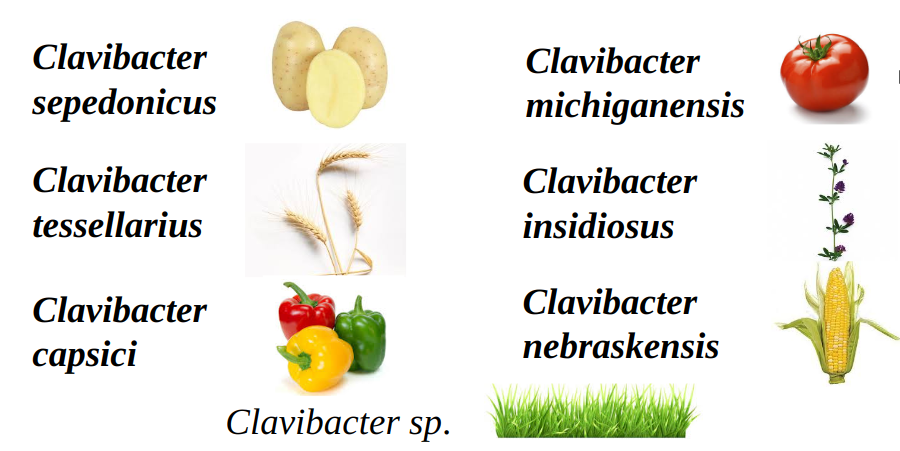
\includegraphics[width=\textwidth]{Img/cap2/clavibacter.png}
%\caption{Clavibacter}
%\end{figure}

\subsection{Comparaciones}


\section{Comparación taxonomica}

\section{Generalizando el N50, nuevas métricas para ensamblados de metagenoma}

En cuanto a la calidad de los ensamblajes, evaluamos la pertinencia de aplicar la métrica genómica N50 a los datos metagenómicos.  \\
(Videvall, 2017)  \\

Se trata de una medida utilizada para evaluar la contigüidad y la calidad del ensamblaje de un genoma. Los contigs de un ensamblaje se ordenan por tamaño y se suman, empezando por el mayor. Se toma el tamaño del contig que hace que el total sea mayor o igual al 50\% del tamaño del genoma.  \\


%\begin{figure}[h]
%\centering
%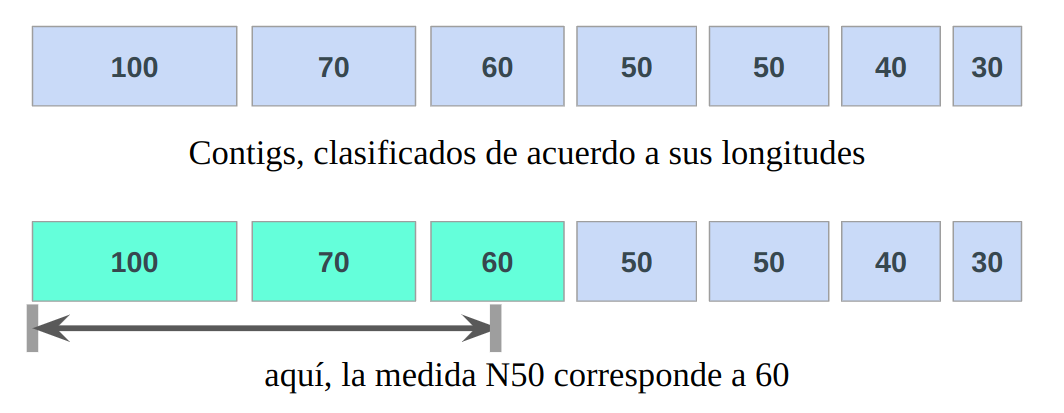
\includegraphics[width=\textwidth]{Img/cap2/N50_es.png}
%\caption{N50 }
%\end{figure}

N50 es una medida de calidad de secuencias genómicas (Miller et al., 2010; Videvall, 2017) (“metagenómica”), la cual se mide ordenando la totalidad de las secuencias de mayor a menor longitud, y sumando todas las longitudes hasta llegar al 50\% del total de la suma; la longitud de la secuencia que esté en este 50\% será la medida N50.  \\

Una medida típica para evaluar el éxito del ensamblaje es la medida N50, que equivale a la longitud del scaffold (o contig) que se solapa con el punto medio de la concatenación de scaffolds (contigs) por orden de longitud. Mäkinen, V., Salmela, L. \& Ylinen, J. Métrica de ensamblaje N50 normalizada mediante encadenamiento colineal restringido por espacios. BMC Bioinformática 13 , 255 (2012). https://doi.org/10.1186/1471-2105-13-255   \\

\thispagestyle{empty}

\chapter{holasss}
\thispagestyle{empty}

\chapter*{Conclusiones}
\thispagestyle{empty}


%----------------------------------------------------------------------------------------
%	APÉNDICES
%----------------------------------------------------------------------------------------

\addtocontents{toc}{\vspace{2em}} % Agrega espacios en la toc

\appendix % Los siguientes capítulos son apéndices

%  Incluye los apéndices en el folder de apéndices

\chapter{Codigos}

Cosas.
\thispagestyle{empty}
\chapter{Imagenes}

Cosas.
\thispagestyle{empty}
%\include{Apendices/AppendixB}
%\include{Apendices/AppendixC}

\addtocontents{toc}{\vspace{2em}} % Agrega espacio en la toc


%----------------------------------------------------------------------------------------
%	BIBLIOGRAFÍA
%----------------------------------------------------------------------------------------
\backmatter
\nocite{*}
\bibliographystyle{apalike}
\bibliography{ref.bib} %Aquí ponen el nombre del archivo .bib






\end{document}